\documentclass[a4paper, 12pt]{article}%тип документа

%отступы
%\usepackage[left=2cm,right=2cm,top=2cm,bottom=3cm,bindingoffset=0cm]{geometry}

%Русский язык
\usepackage[T2A]{fontenc} %кодировка
\usepackage[utf8]{inputenc} %кодировка исходного кода
\usepackage[english,russian]{babel} %локализация и переносы

%абзац
\usepackage{lipsum}
\setlength{\parindent}{5ex}
\setlength{\parskip}{1em}

%Вставка картинок
\usepackage{wrapfig}
\usepackage{graphicx}
\usepackage{placeins}
\graphicspath{{pictures/}}
\DeclareGraphicsExtensions{.pdf,.png,.jpg}

%оглавление
\usepackage{titlesec}
\titlespacing{\chapter}{0pt}{-30pt}{12pt}
\titlespacing{\section}{\parindent}{5mm}{5mm}
\titlespacing{\subsection}{\parindent}{5mm}{5mm}
\usepackage{setspace}

%Графики
\usepackage{multirow}
\usepackage{pgfplots}
\pgfplotsset{compat=1.9}

%Математика
\usepackage{amsmath, amsfonts, amssymb, amsthm, mathtools}

\begin{document}

\begin{titlepage}

\begin{center}
%\vspace*{1cm}
\large\textbf{Московский Физико-Технический Институт}\\
\large\textbf{(государственный университет)}
\vfill
\line(1,0){430}\\[1mm]
\huge\textbf{Работа 20}\\
\line(1,0){430}\\[1mm]
\vfill
\large Сибгатуллин Булат, ФРКТ\\
\end{center}

\end{titlepage}

\section{}

\subsection{\textbf{model1\_1}}

\subsubsection{}

Исследуем модель резистора как источника шумового напряжения, изучим зависимость шумового напряжения от R, получим что шум растет как $\sqrt{R}$.

\begin{figure}[h!]
    \centering
    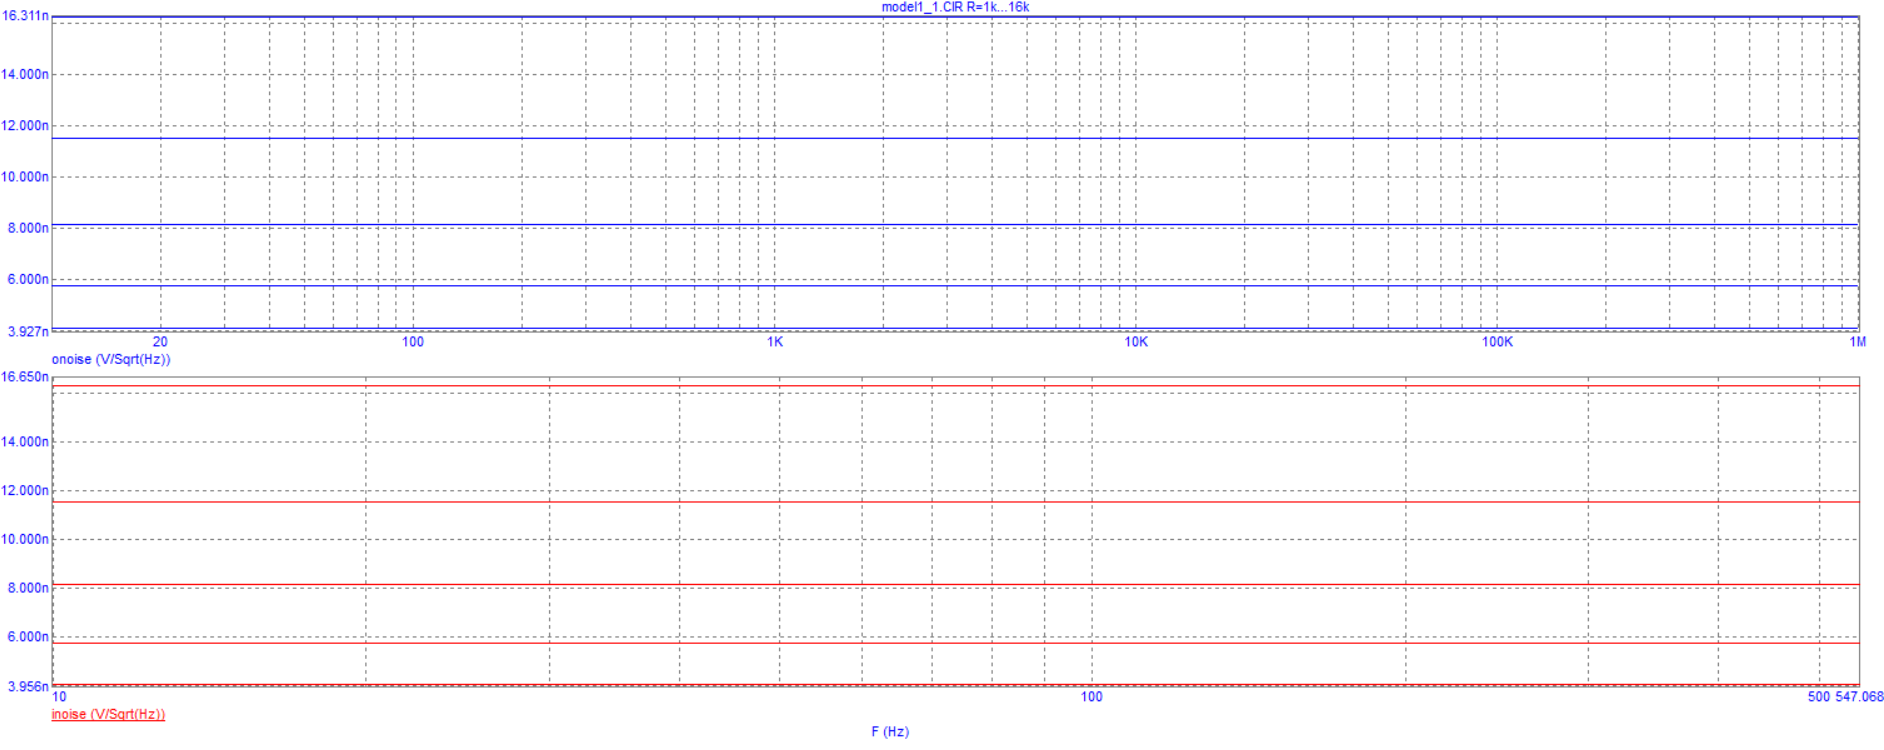
\includegraphics[scale = 0.4 \textwidth]{images/mod1_1_1_2.png}
    \caption{Зависимость шумового напряжения от R}
    \label{fig:eR}
\end{figure}

\subsubsection{}

Измерим уровень шума $\sigma$ на выводе резистора в полосе F = 1 МГц.

\begin{figure}[h!]
    \centering
    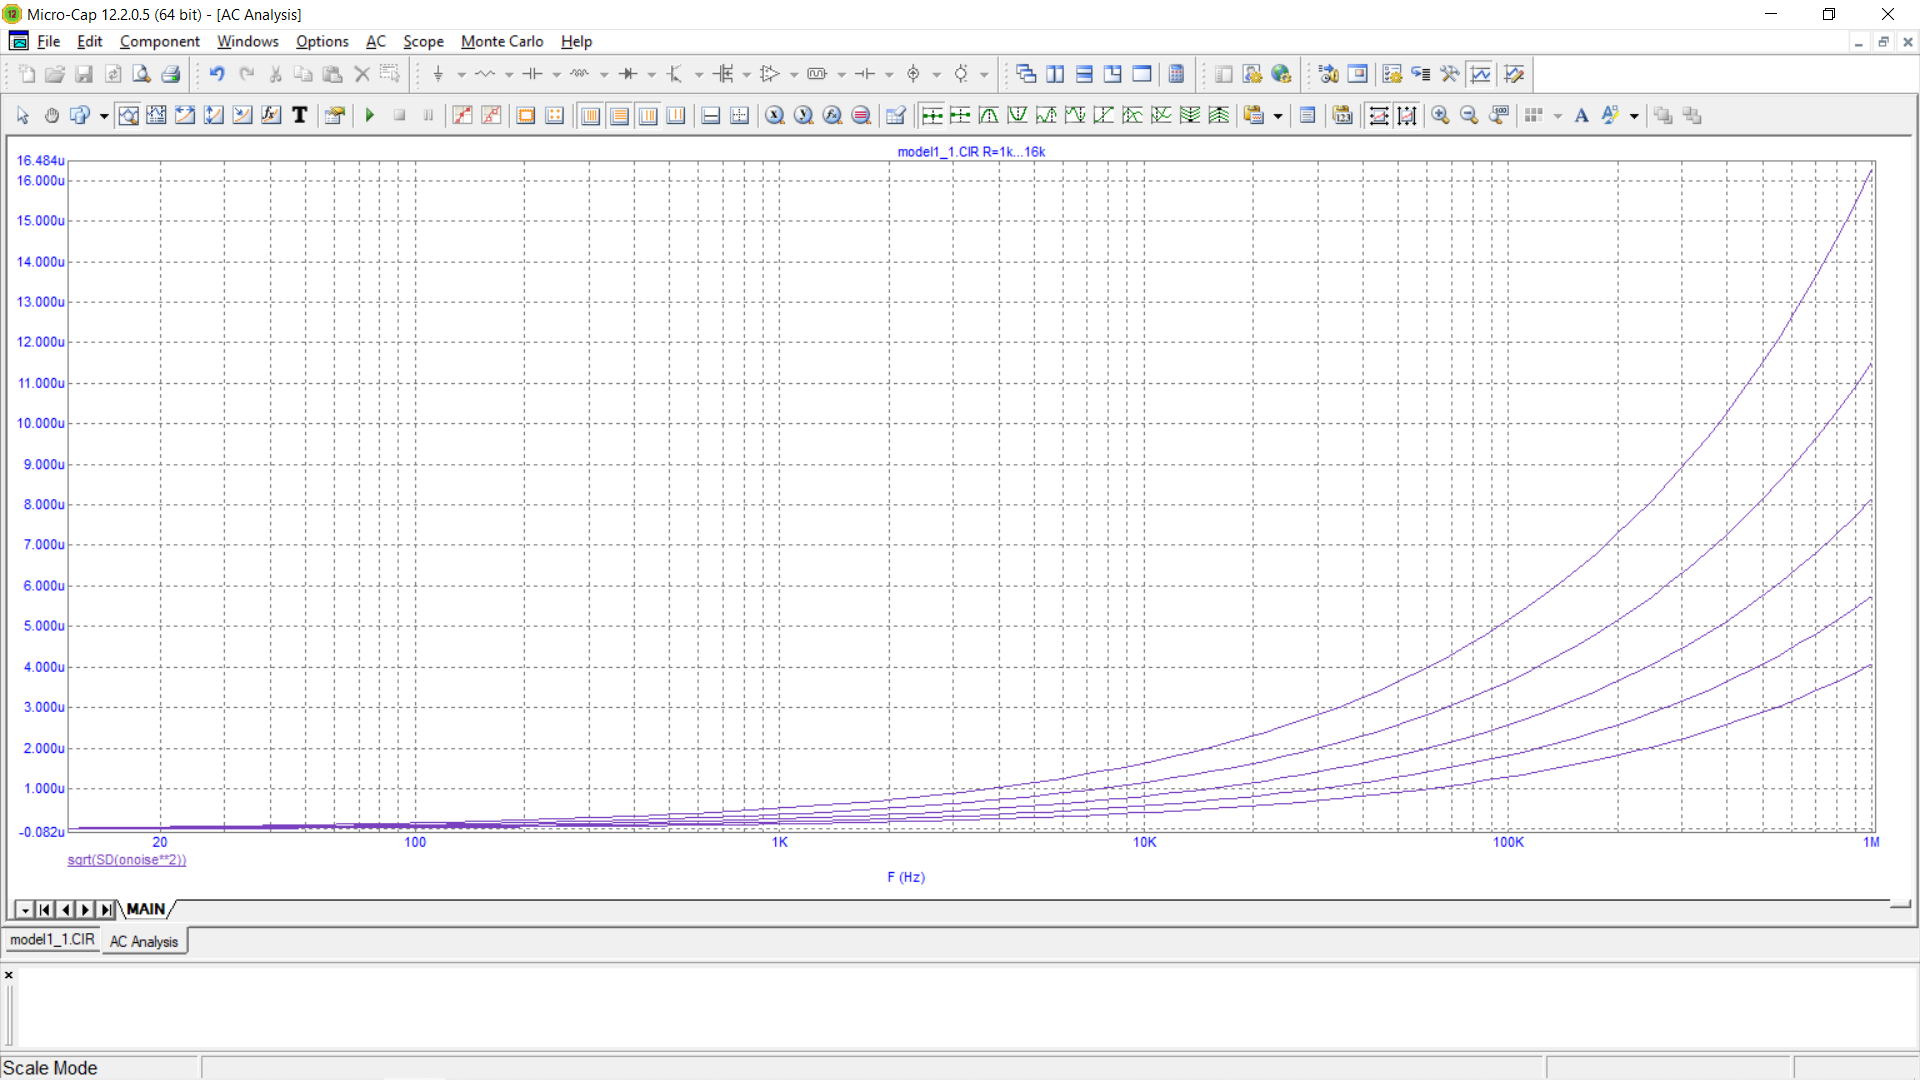
\includegraphics[scale = 0.4 \textwidth]{images/mod1_1_2_1.png}
    \caption{R = [1k, 16k| Log2]}
    \label{fig:R16}
\end{figure}

\begin{figure}[h!]
    \centering
    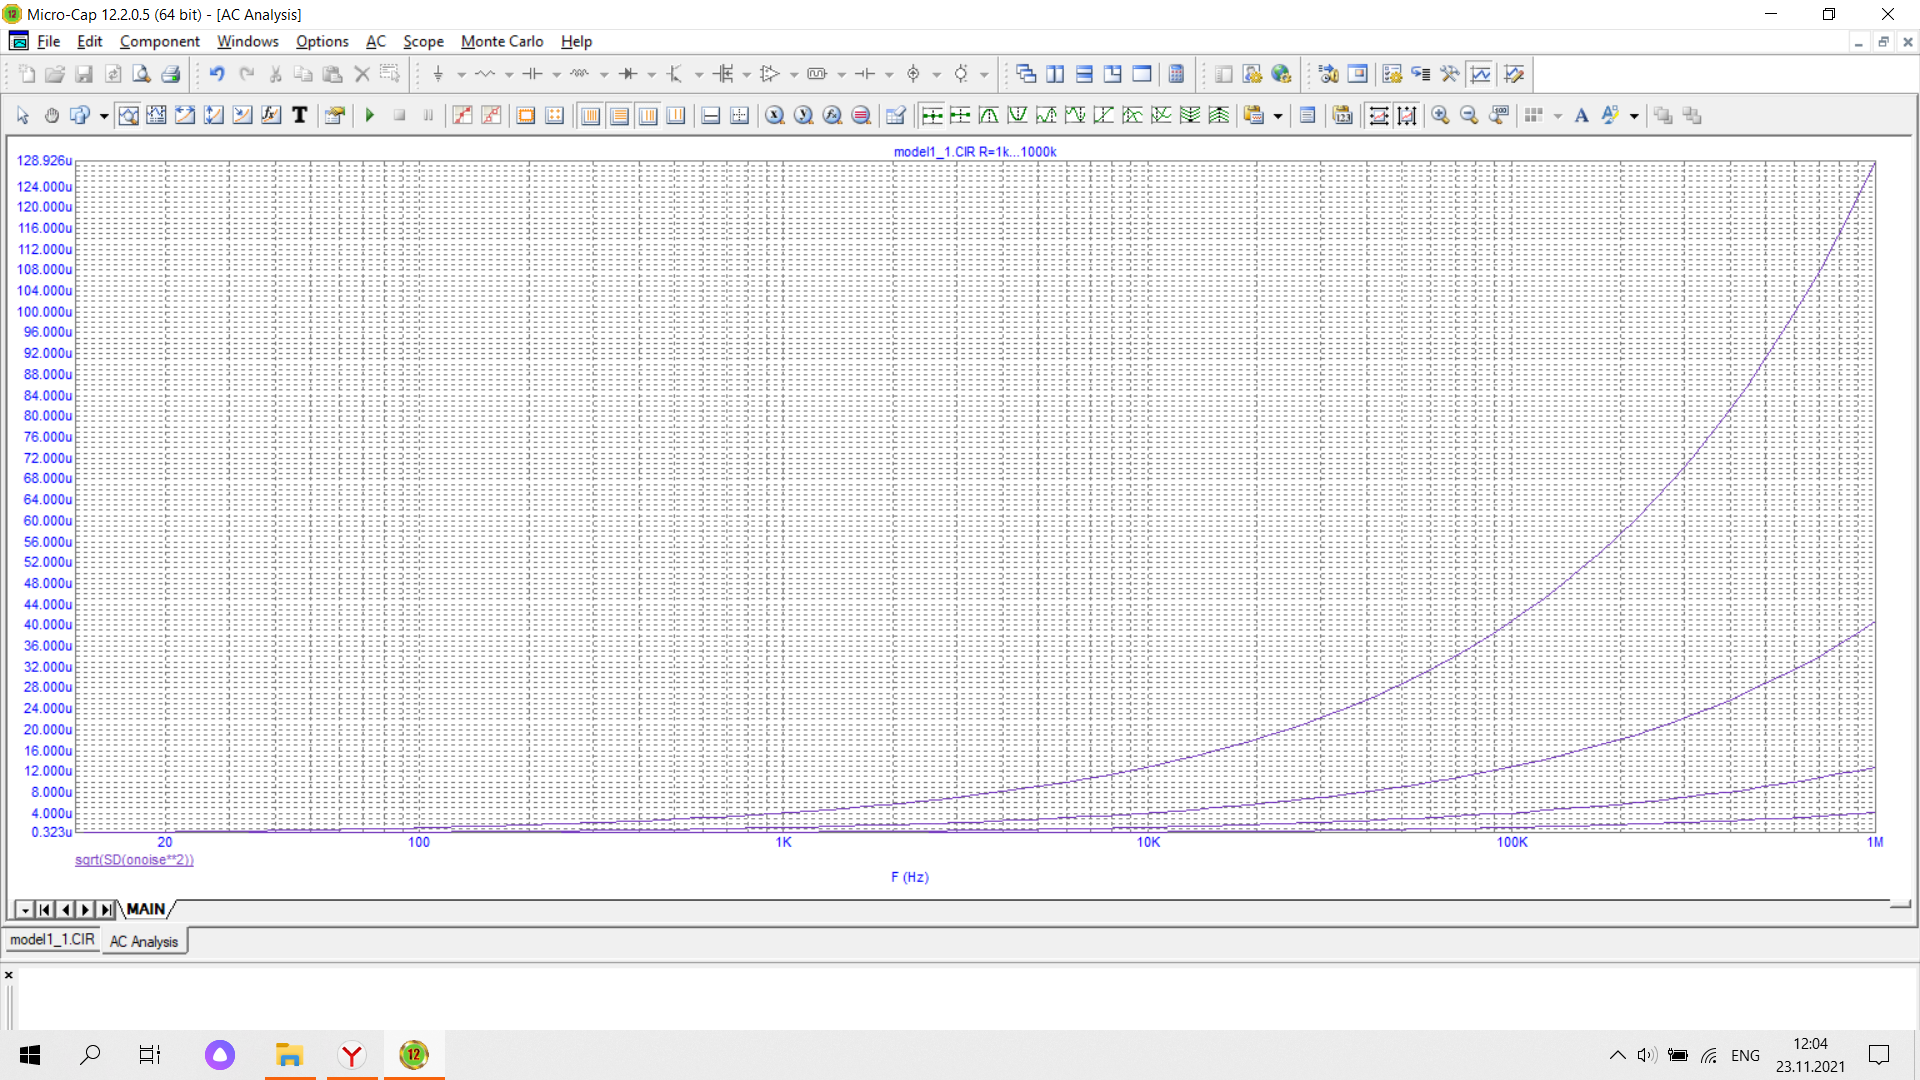
\includegraphics[scale = 0.4 \textwidth]{images/mod1_1_2_2.png}
    \caption{R = [1k, 1000k| Log10]}
    \label{fig:R1000}
\end{figure}

\begin{table}[h!]
    \centering
    \begin{tabular}{|c|c|c|c|c|c|c|c|c|} \hline
        R & 1k & 2k & 4k & 8k & 16k & 10k & 100k & 1000k\\ \hline
        $\sigma$ & 4u & 5,7u & 8u & 11,4u & 16u & 12,7u & 40u & 128u\\ \hline
    \end{tabular}
    \caption{Зависимость уровня шума $\sigma$ от R}
    \label{tab:sR}
\end{table}

\subsubsection{}

Перейдем к модели источника тока, получаем, что с увеличением R1 ток остается нулевым, а напряжение растет как $\sqrt{R}$.

\begin{figure}[h!]
    \centering
    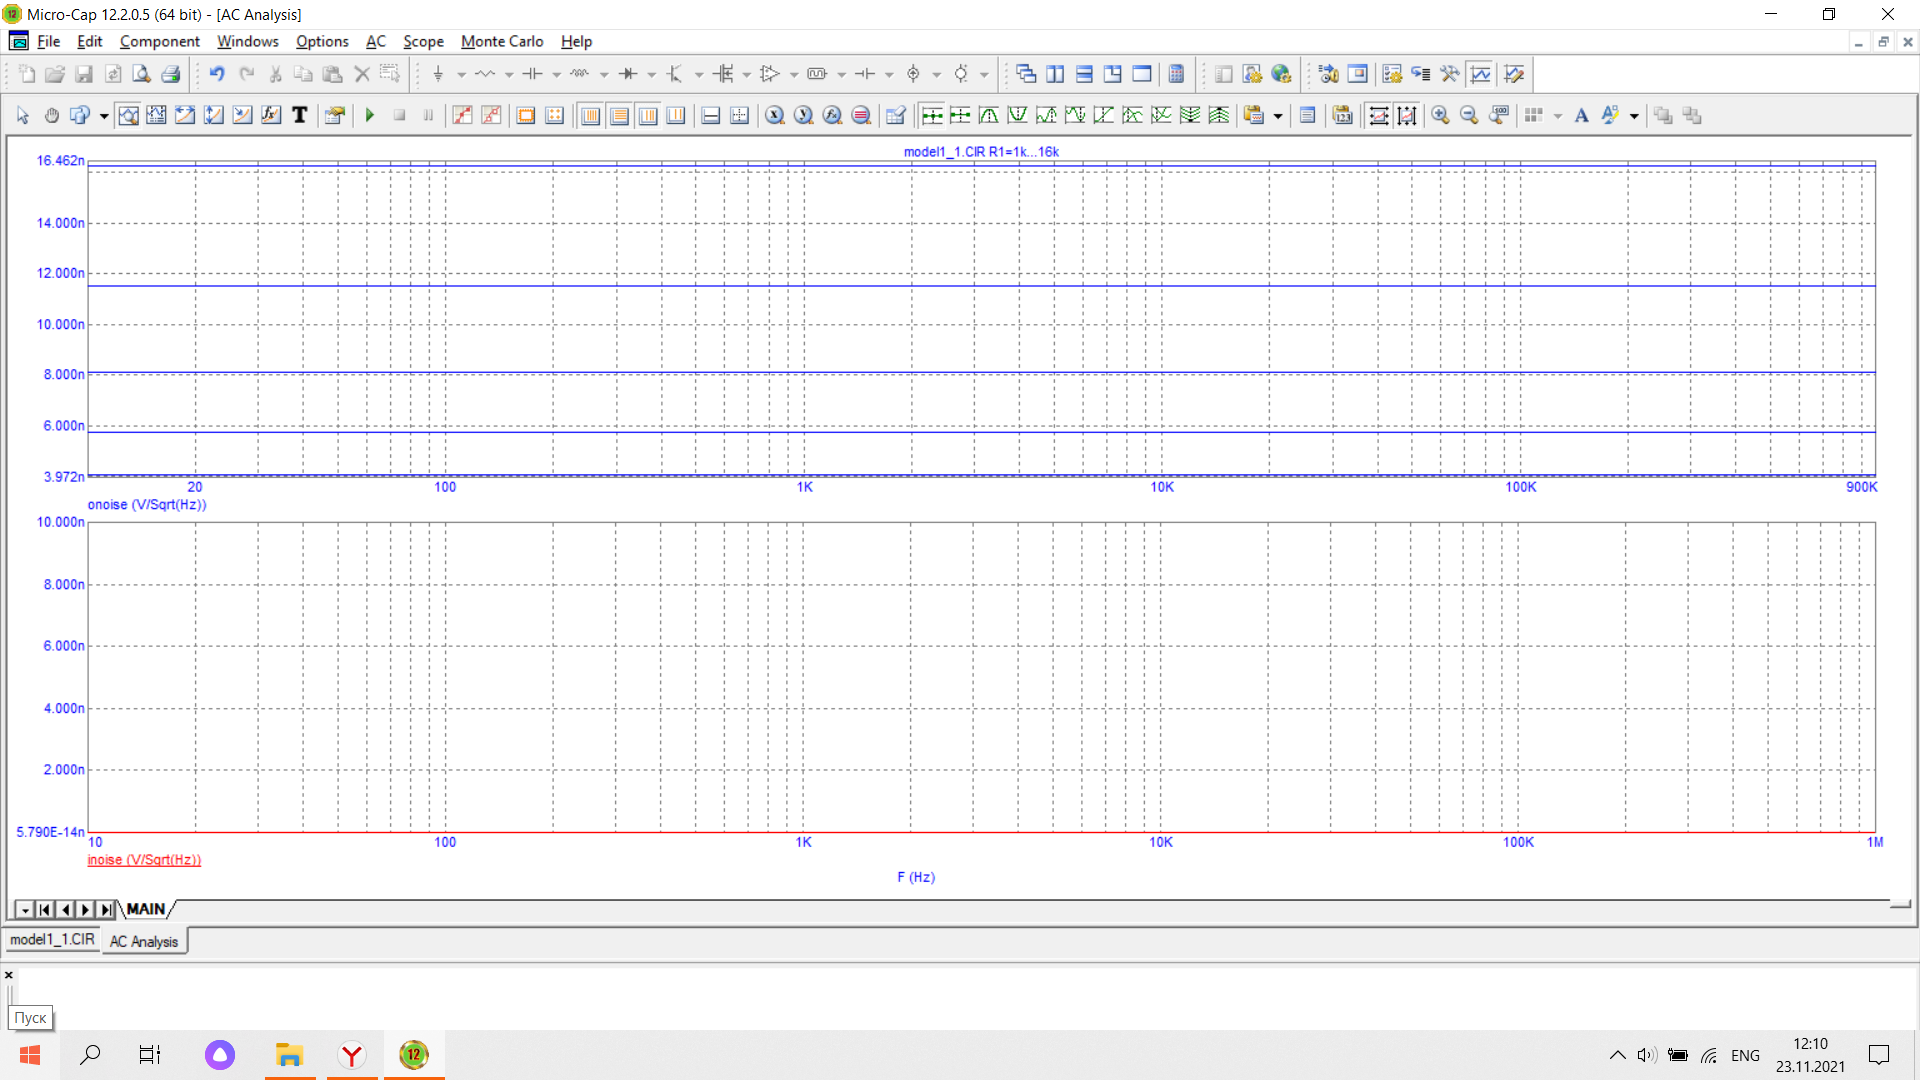
\includegraphics[scale = 0.4 \textwidth]{images/mod1_1_3.png}
    \caption{Шумовые напряжение и ток в модели с источником тока}
    \label{fig:R3}
\end{figure}

\subsection{\textbf{model1\_2}}

\subsubsection{}

Изучим шумы в схеме с последовательным соединением, проверим закон сложения шумовых напряжений.

\begin{figure}[h!]
    \centering
    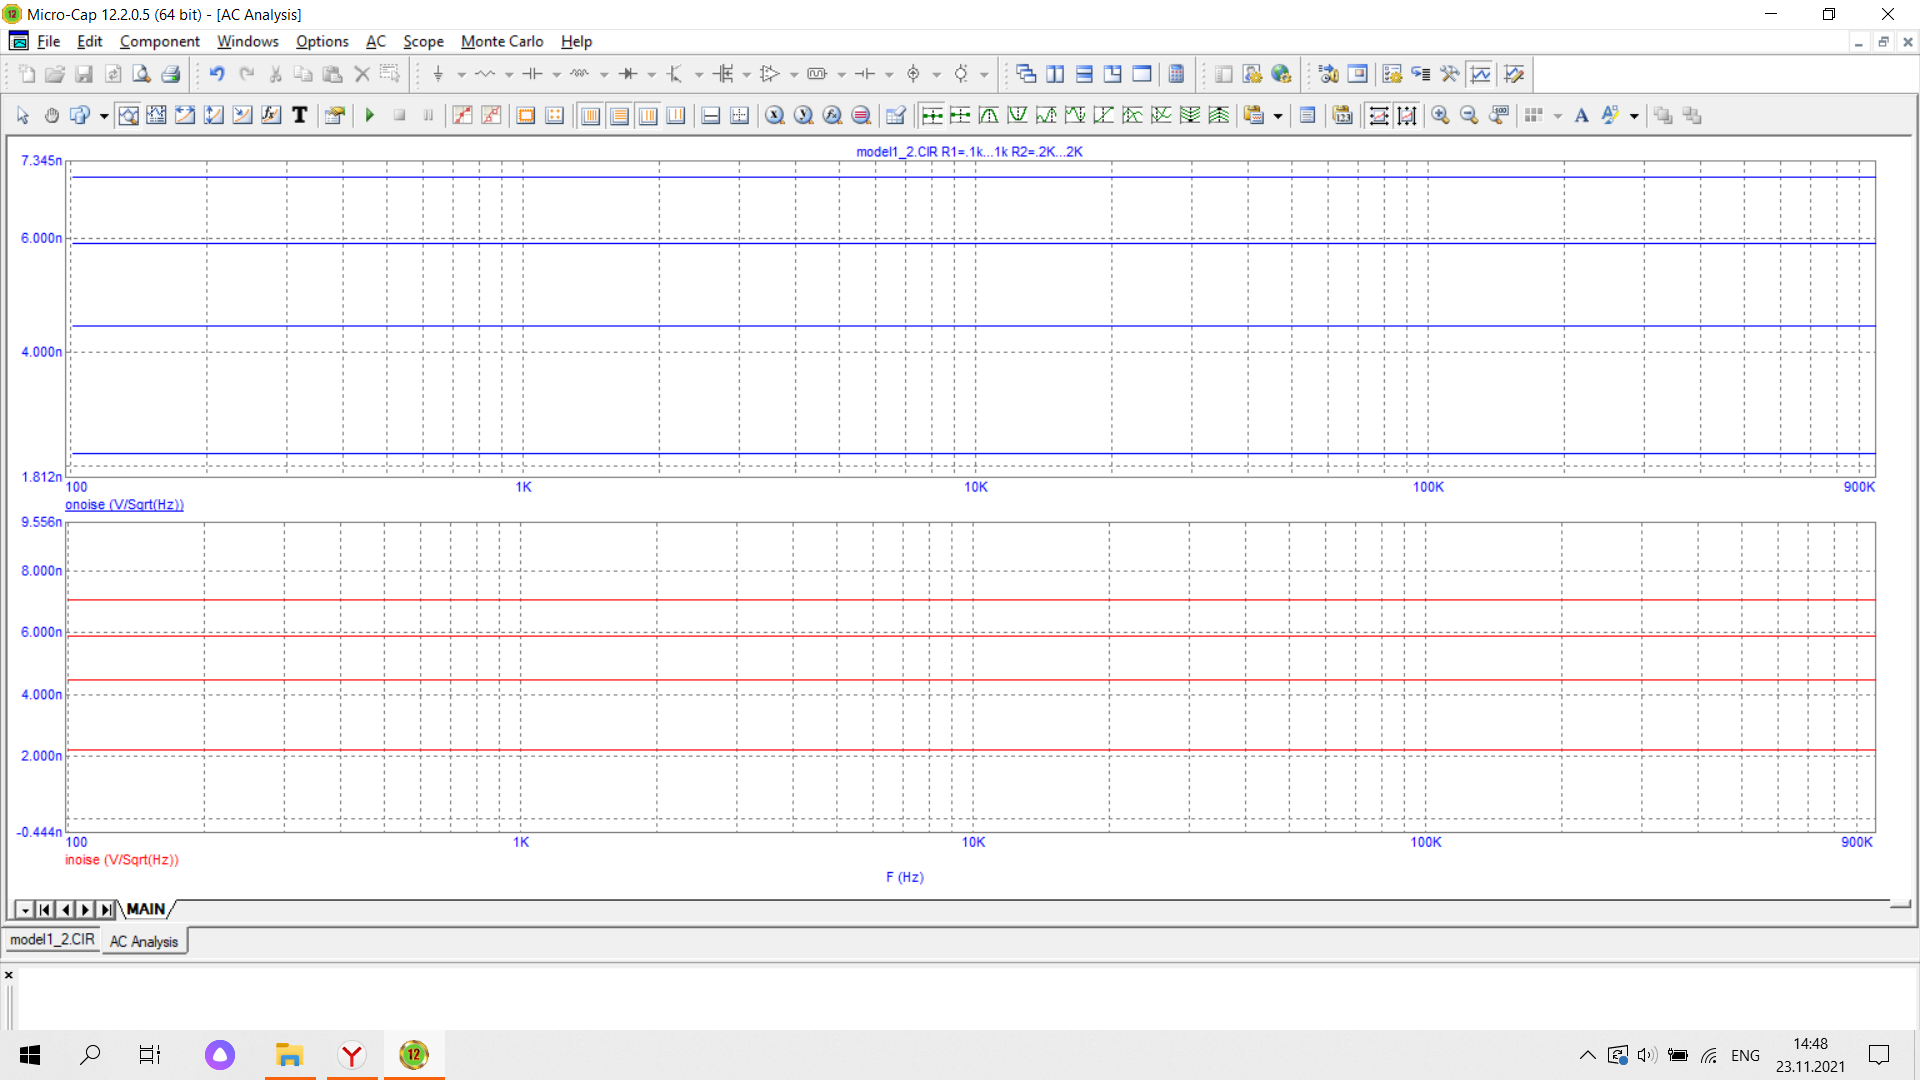
\includegraphics[scale = 0.4 \textwidth]{images/mod1_2_1.png}
    \caption{Варьирование R = [0,1k, 1k| 1k], R = [0,2k, 2k| 2k]}
    \label{fig:1_2_1}
\end{figure}

Закон сложения шумовых напряжений выполняется.

\subsubsection{}
 
Перейдем к схеме с параллельным соединением.

\begin{figure}[h!]
    \centering
    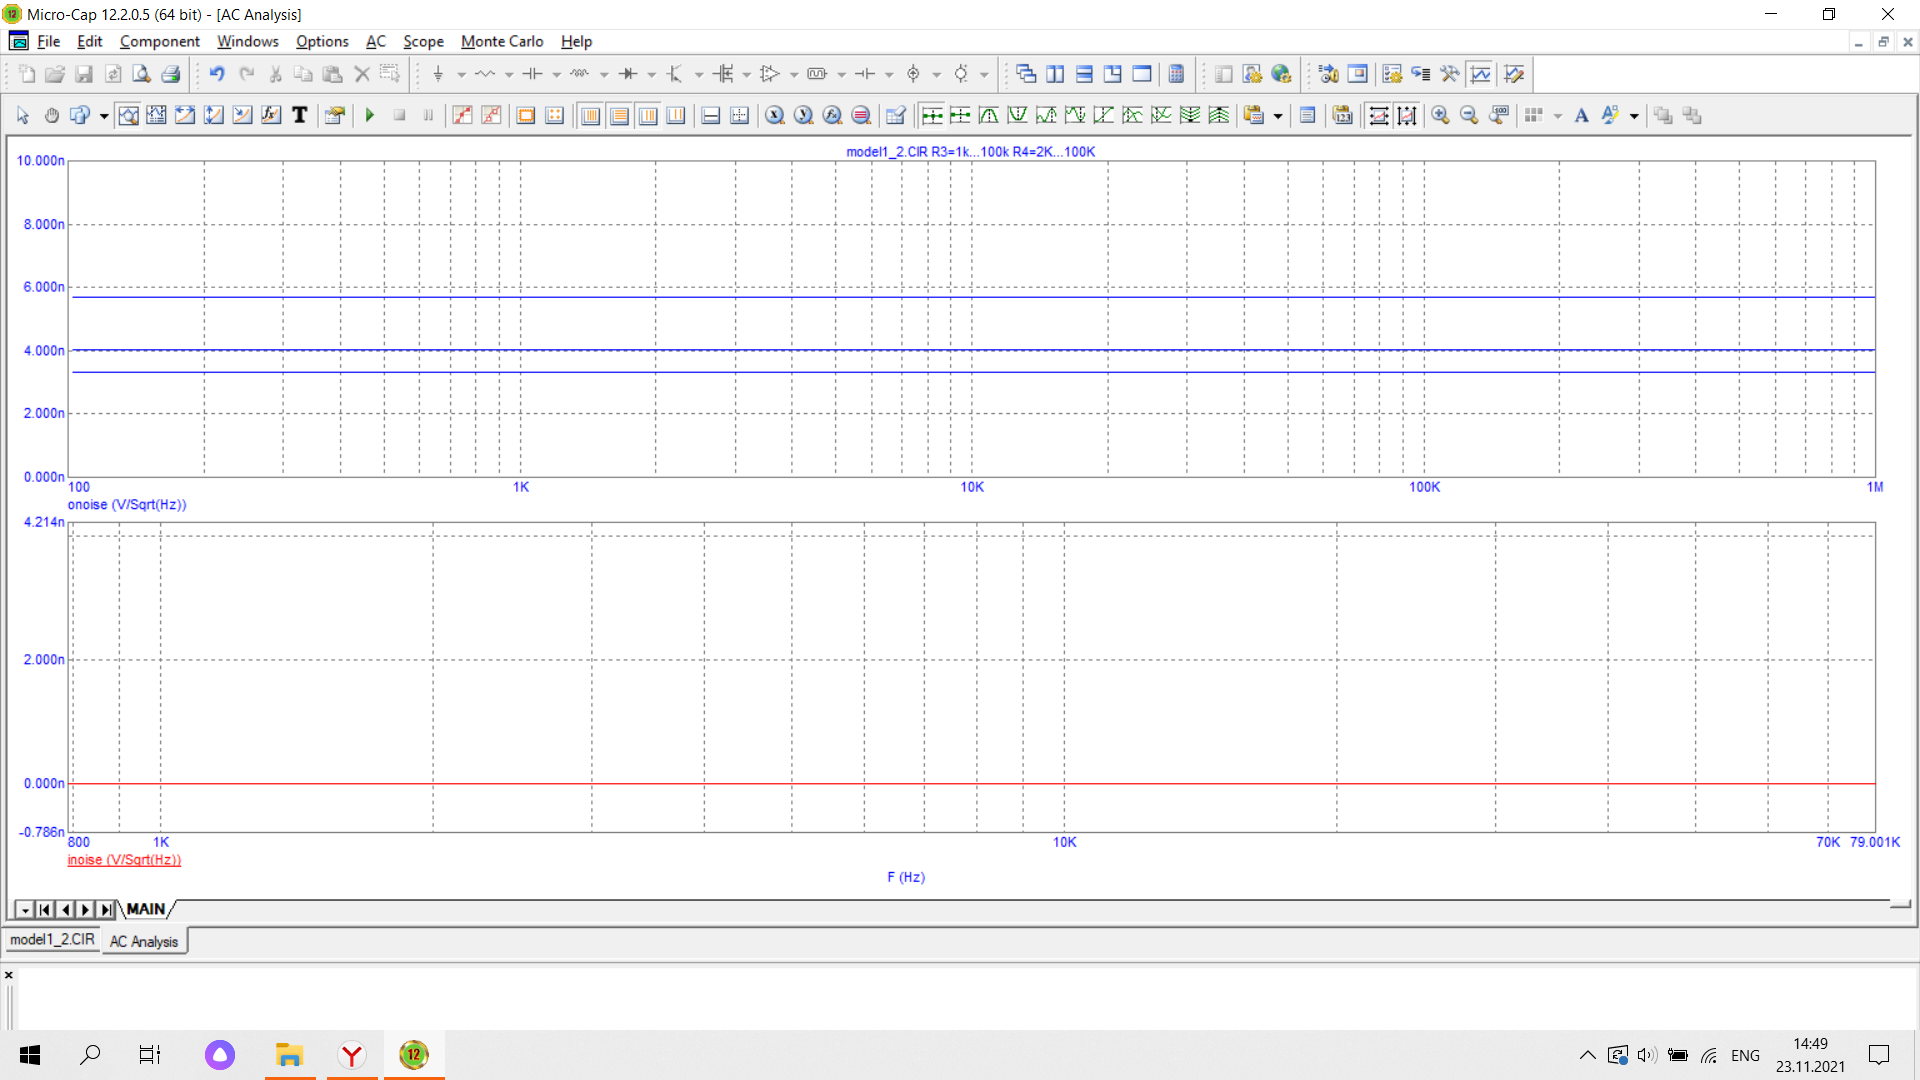
\includegraphics[scale = 0.4 \textwidth]{images/mod1_2_2.png}
    \caption{Варьирование R = [1k, 100k| 99k], R = [2k, 100k| 98k]}
    \label{fig:1_2_2}
\end{figure}

\subsection{\textbf{model1\_3}}

\subsubsection{}

Измерим шумовое напряжение в узле $n(f) = 5,2 \text{ нB}\sqrt{\text{Гц}}$. 

\pgfplotstableread[col sep = semicolon]{KT.csv}{\tabl}

\begin{figure}[h!]
    \centering
    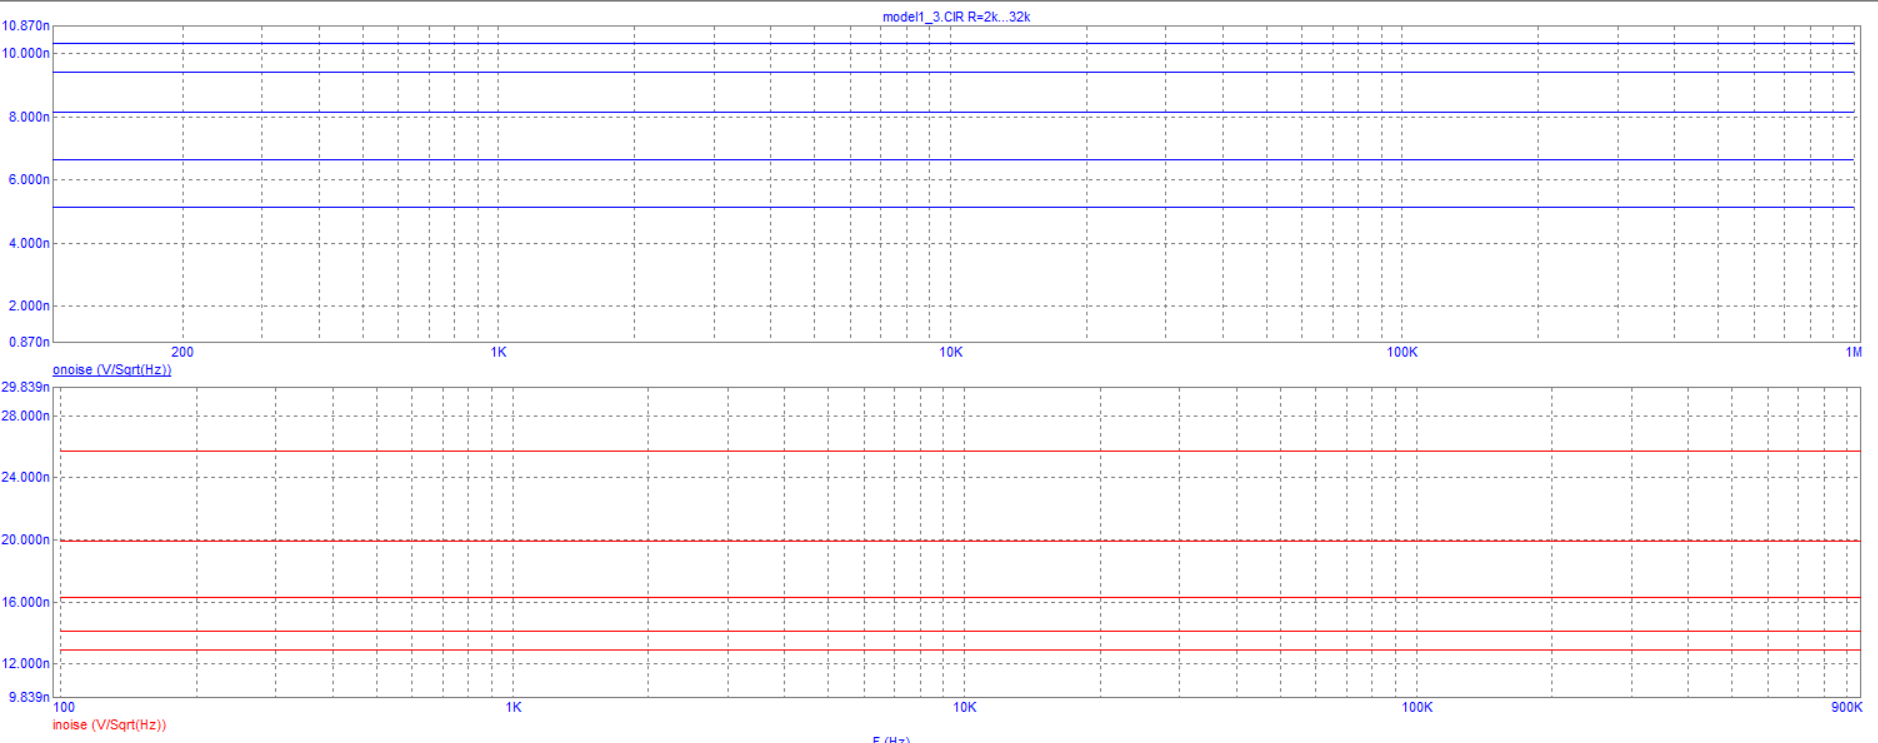
\includegraphics[scale = 0.4 \textwidth]{images/mod1_3_1.png}
    \caption{Приведенное ко входу напряжение $e_n$ от R}
    \label{fig:1_3_1}
\end{figure}

\begin{tikzpicture}
\begin{axis}[title = $K_n(R)$,]
\addplot table [x={R}, y={K}] {\tabl};
\end{axis}
\centering
\end{tikzpicture}

\begin{tikzpicture}
\centering
\begin{axis} [title = $T_n(R)$]
\addplot table [x={R}, y={T}] {\tabl};
\end{axis}
\end{tikzpicture}

\subsubsection{} 

Исключим резистор R и поставим вместо него нешумящий резистор H. 

\begin{figure}[h!]
    \centering
    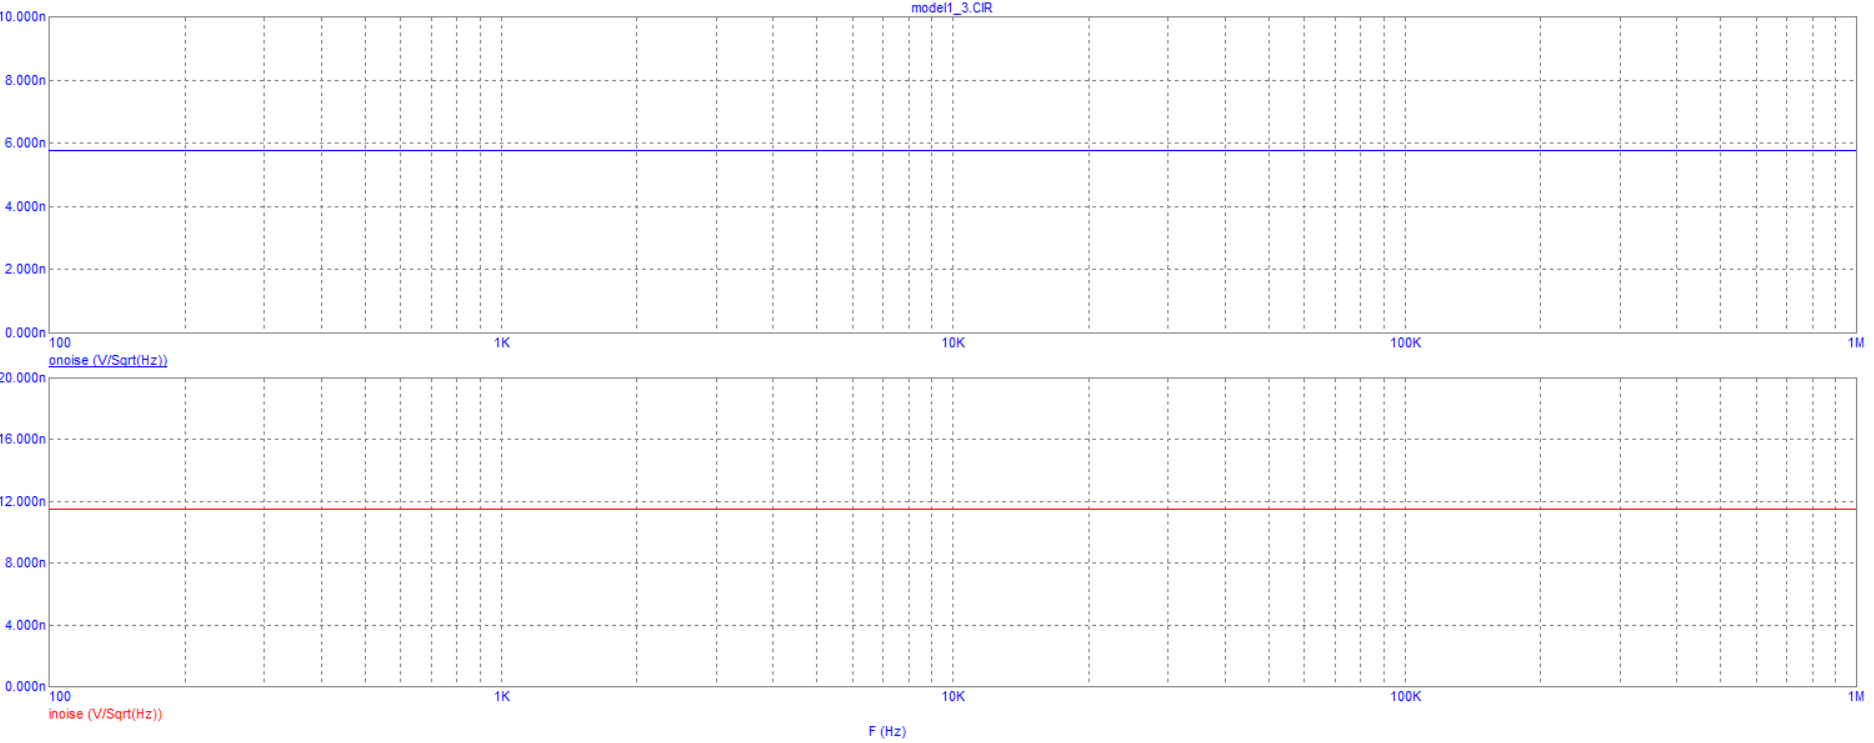
\includegraphics[scale = 0.4 \textwidth]{images/mod1_3_2.png}
    \caption{Нешумящий резистор}
\end{figure}

\section{\textbf{model2}}

\subsection{}

\begin{figure}[h!]
    \centering
    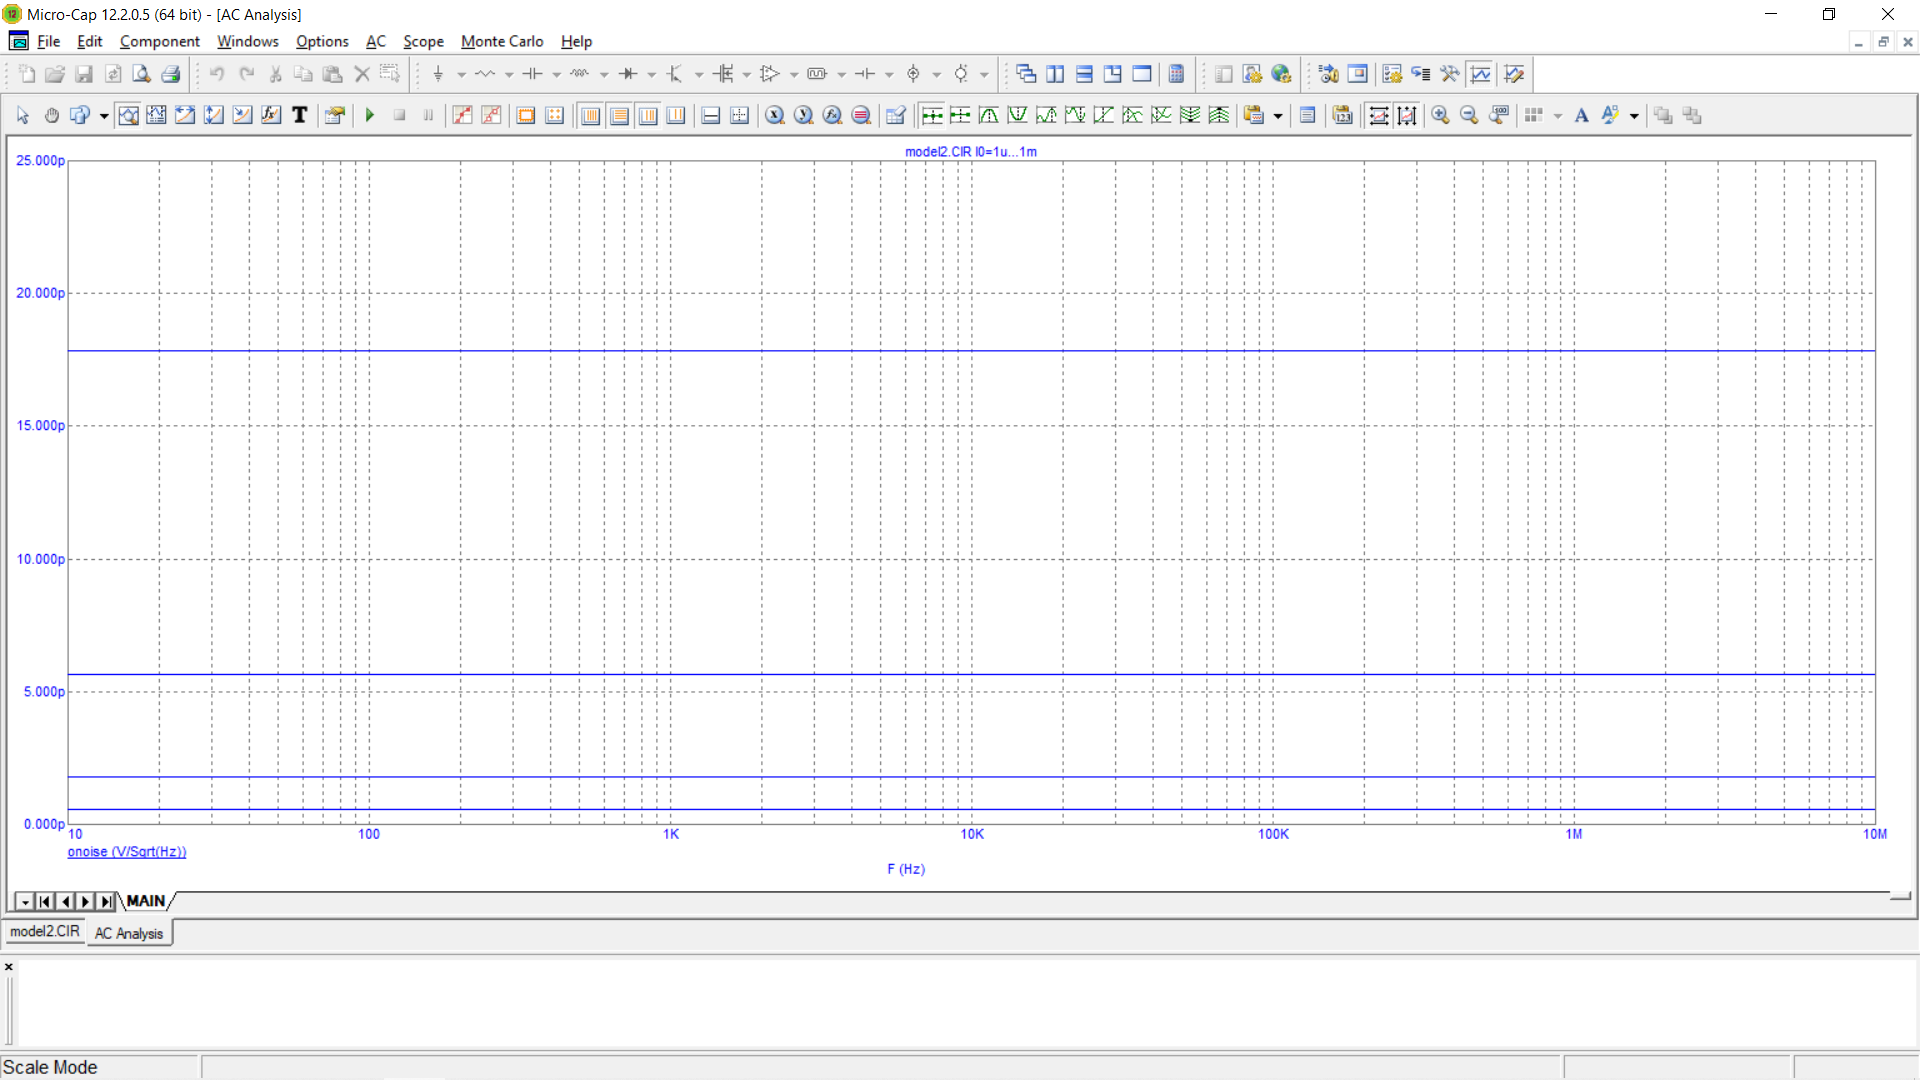
\includegraphics[scale = 0.4 \textwidth]{images/mod2_1_1.png}
    \caption{Микротоки}
    \label{fig:m211}
\end{figure}

Проверим выполнение закона $\sqrt{I_0}$:
\begin{itemize}
    \item $I_{01} = 1\mu$ => $e_{01} = 564f$;
    \item $I_{02} = 10\mu$ => $e_{02} = 1.69p \approx \sqrt{10}e_{01}$;
    \item $I_{03} = 100\mu$ => $e_{03} = 5.603p \approx \sqrt{100}e_{01}$; 
    \item $I_{04} = 1000\mu$ => $e_{04} = 17.79p \approx \sqrt{1000}e_{01}$;
\end{itemize}

\begin{figure}[h!]
    \centering
    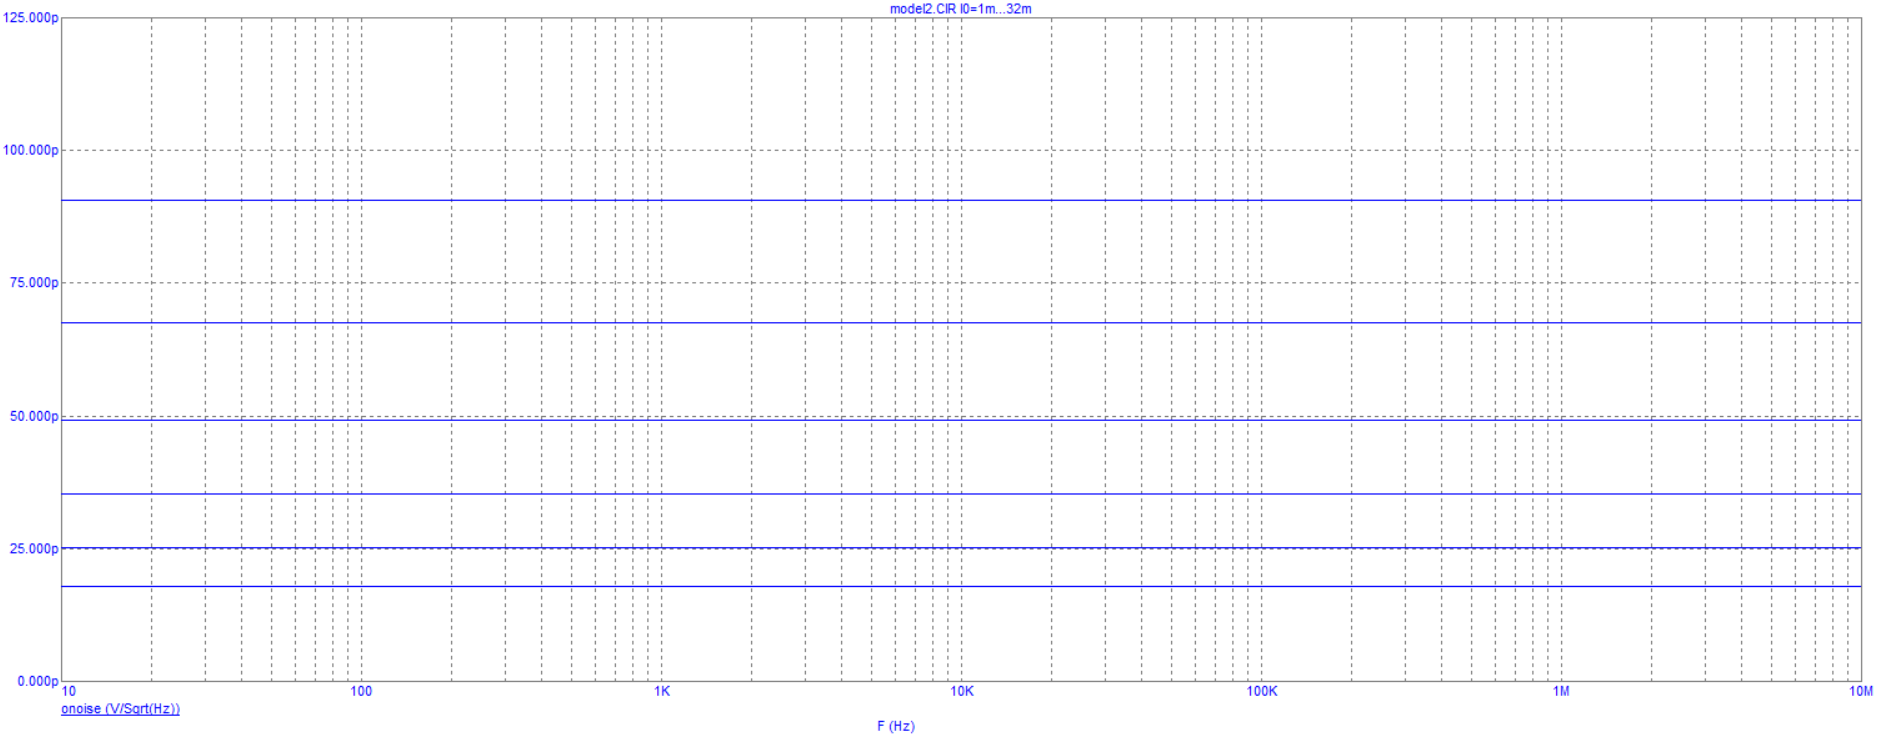
\includegraphics[scale = 0.4 \textwidth]{images/mod2_1_2.png}
    \caption{Умеренные токи}
    \label{fig:m212}
\end{figure}

Проверим выполнение закона $\sqrt{I_0}$:
\begin{itemize}
    \item $I_{01} = 1\mu$ => $e_{01} = 17.89p$;
    \item $I_{02} = 2\mu$ => $e_{02} = 25.18p \approx \sqrt{2}e_{01}$;
    \item $I_{03} = 4\mu$ => $e_{03} = 35.31p \approx \sqrt{4}e_{01}$; 
    \item $I_{04} = 8\mu$ => $e_{04} = 49.20p \approx \sqrt{8}e_{01}$;
    \item $I_{05} = 16\mu$ => $e_{05} = 67.56p \approx \sqrt{16}e_{01}$;
    \item $I_{06} = 32\mu$ => $e_{06} = 92.61p \approx \sqrt{32}e_{01}$;
\end{itemize}

Напряжение пробоя диода???

\subsection{}

\begin{figure}[h!]
    \centering
    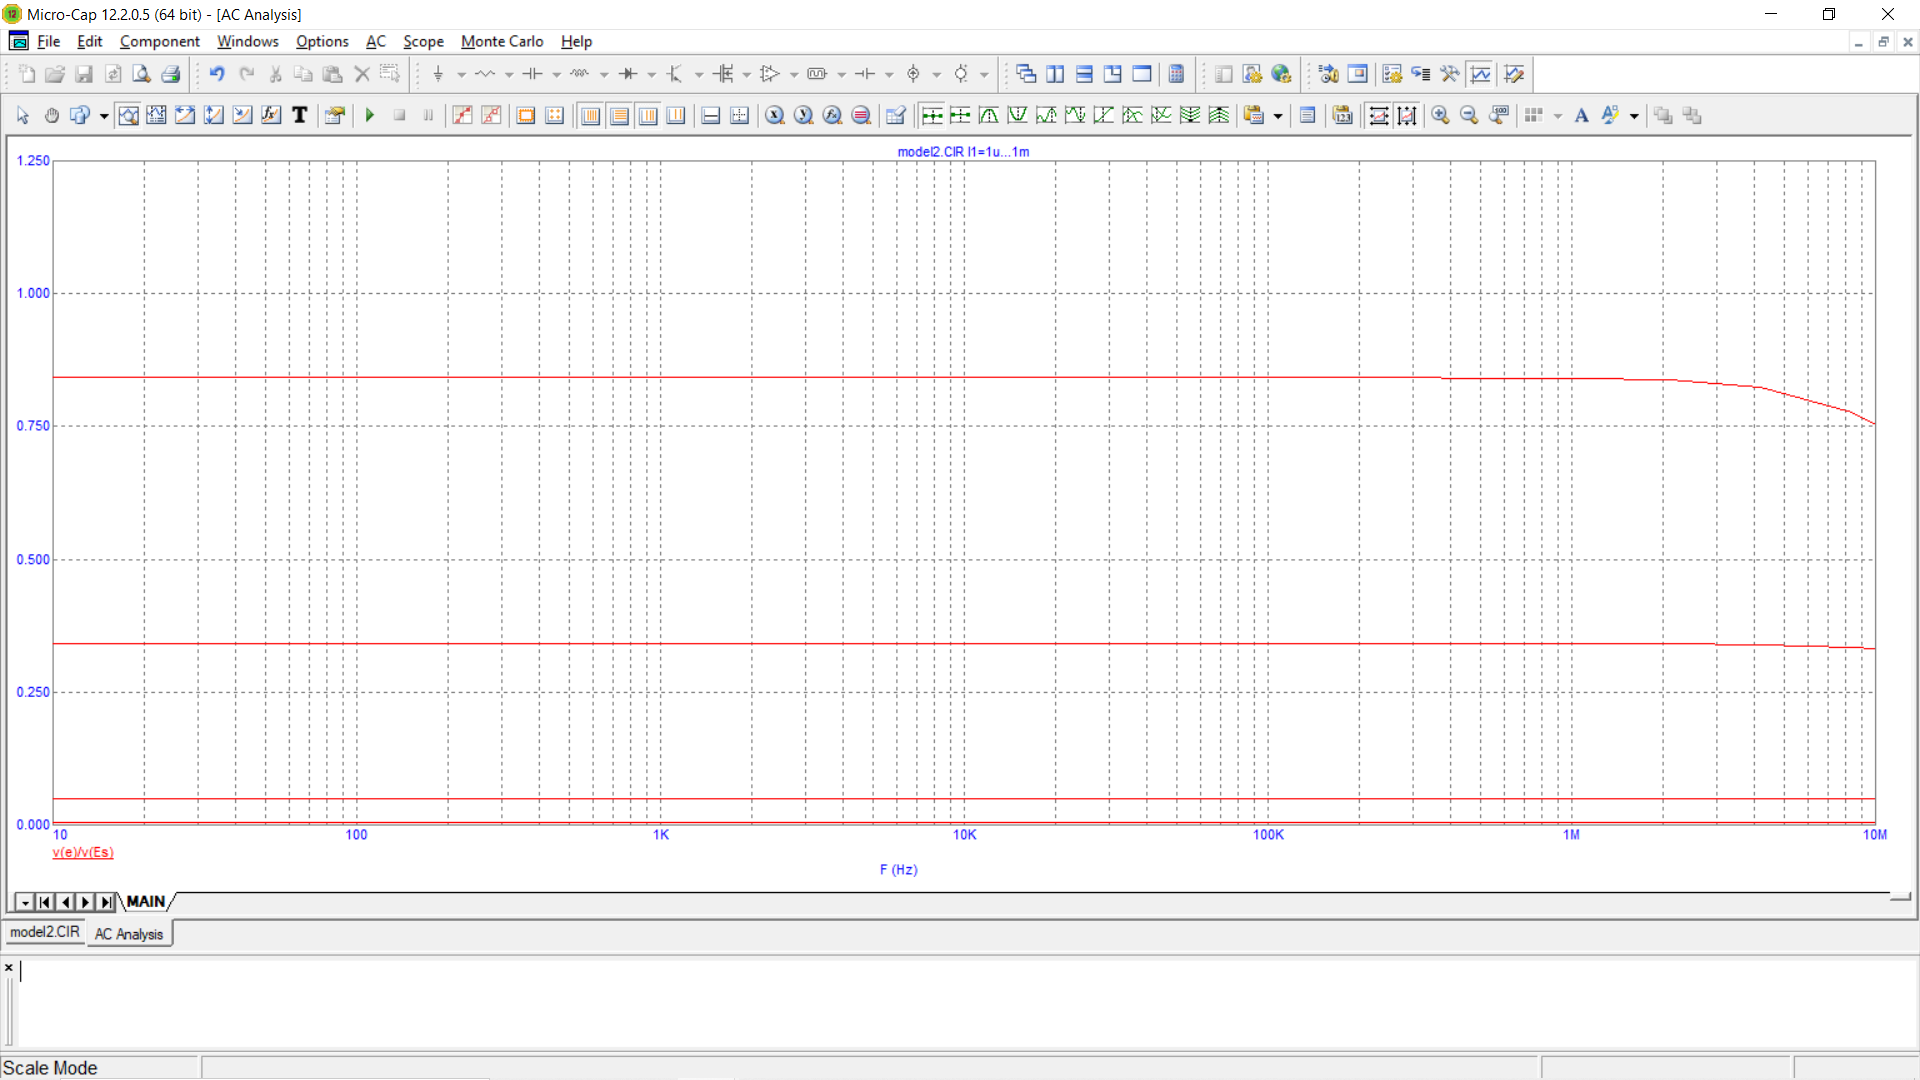
\includegraphics[scale = 0.4 \textwidth]{images/mod2_2.png}
    \caption{$K = r_d/(R_1 + r_d)$}
    \label{fig:m212}
\end{figure}

Найдем $r_d$ как $r_d \approx K R_1$, $R_1 = 10k$:

\begin{itemize}
    \item $I_{01} = 1\mu$ => $K_{1} = 5.16m$ => $r_d = 51.6$ Ом;
    \item $I_{02} = 10\mu$ => $K_{2} = 49.24m$ => $r_d = 492.4$ Ом;
    \item $I_{03} = 100\mu$ => $K_{3} = 341.56m$ => $r_d = 3415.6$ Ом;
    \item $I_{04} = 1m$ => $K_{4} = 841.71m$ => $r_d = 8417.1$ Ом;
\end{itemize}

\subsection{}

\begin{figure}[h!]
    \centering
    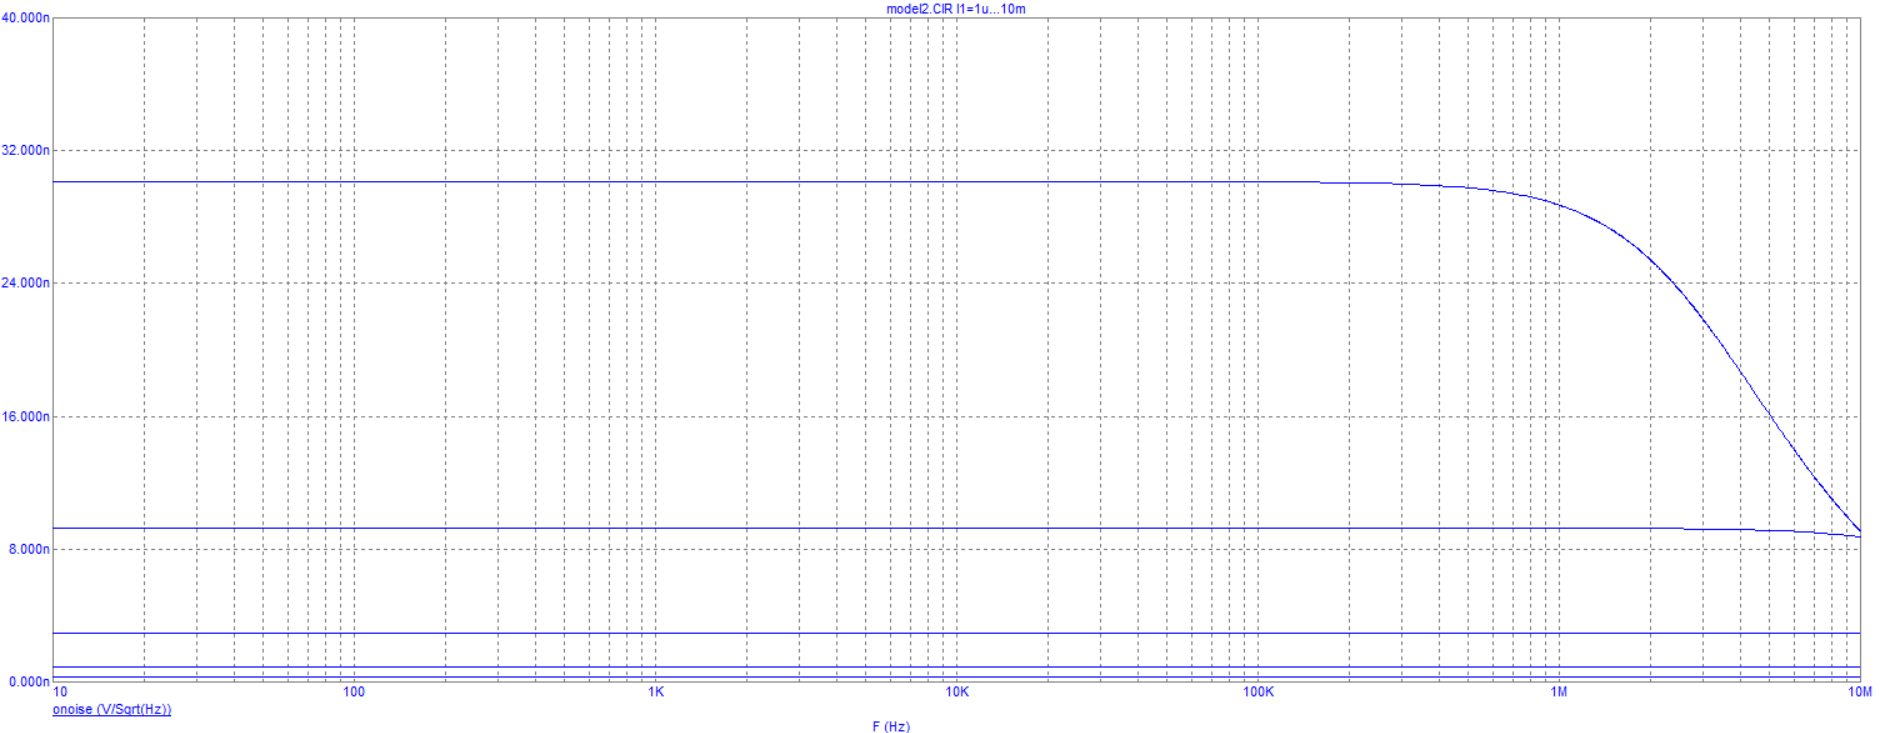
\includegraphics[scale = 0.4 \textwidth]{images/mod2_3.png}
    \caption{e(f) для I = [1u, 10m|Log10]}
    \label{fig:m23}
\end{figure}

Проверим формулу $e(f) = i(f)r_d$, возьмем $i(f) = \sqrt{2*e*I_1}$:
\begin{itemize}
    \item $I_{01} = 1\mu$ => $e(f)_\text{теор} = 29.2n$, $e(f)_\text{прак} = 30.1n$;
    \item $I_{02} = 10\mu$ => $e(f)_\text{теор} = 8.8n$, $e(f)_\text{прак} = 9.3n$;
    \item $I_{03} = 100\mu$ => $e(f)_\text{теор} = 2.7n$, $e(f)_\text{прак} = 2.9n$;
    \item $I_{04} = 1m$ => $e(f)_\text{теор} = 1005p$, $e(f)_\text{прак} = 928p$;
    \item $I_{05} = 10m$ => $e(f)_\text{теор} = 410n$, $e(f)_\text{прак} = 304p$;
\end{itemize}

\section{\textbf{model3}}

\subsection{Интегрирующая цепь}

\begin{figure}[h!]
    \centering
    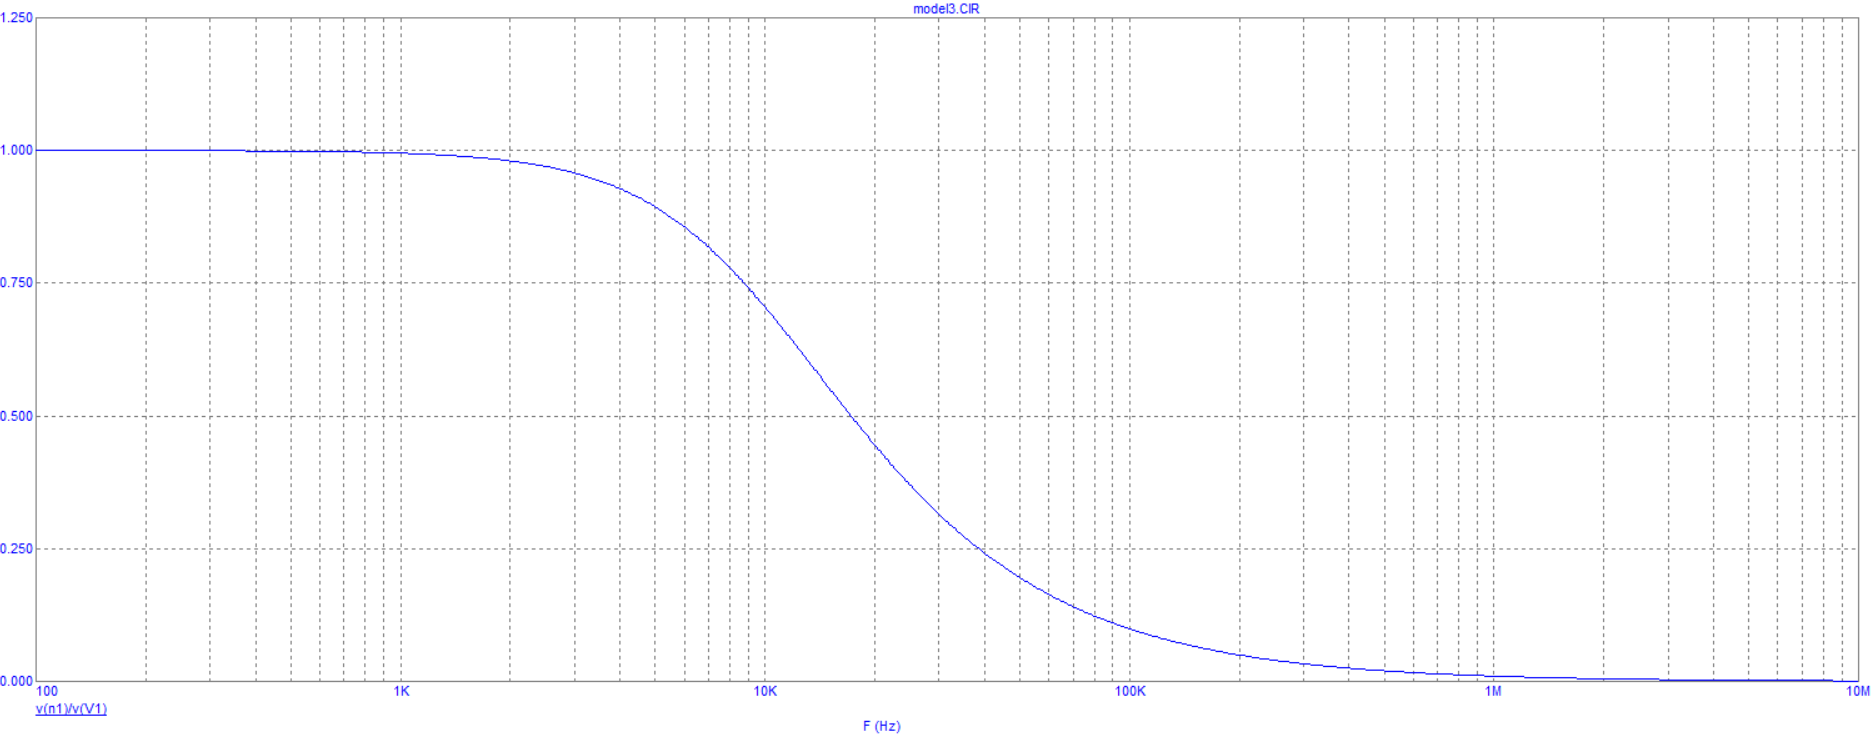
\includegraphics[scale = 0.4 \textwidth]{images/mod3_1_1.png}
    \caption{Граничная частота $f_h = 10$}
    \label{fig:m311}
\end{figure}

$\sigma_\text{теор1} = n1\sqrt{Fn} = 12.8n\sqrt{\pi/2 \cdot 10000} = 1.63\mu$
$\sigma_\text{теор2} = \sqrt{\frac{kT}{C}} = 1.61\mu$
$\sigma_\text{прак} = 1.60\mu$

\begin{figure}[h!]
    \centering
    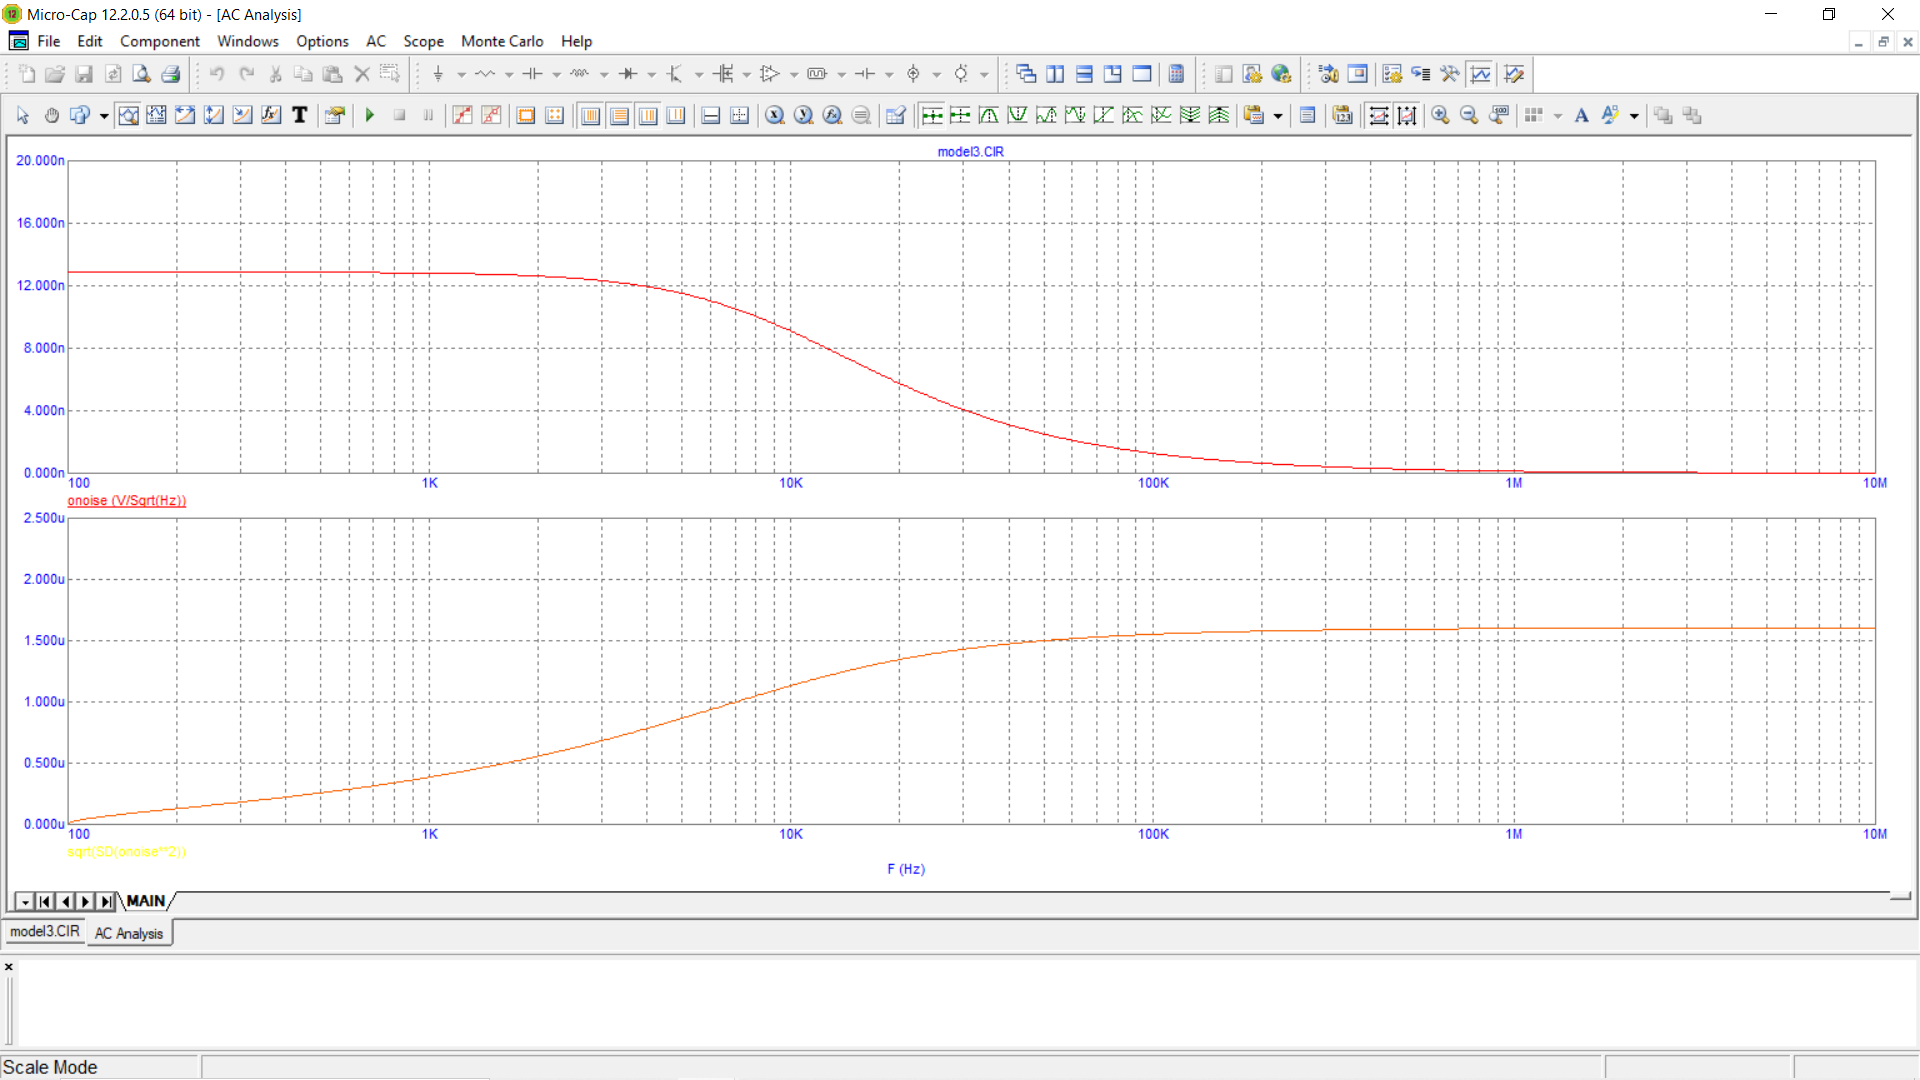
\includegraphics[scale = 0.4 \textwidth]{images/mod3_1_2.png}
    \caption{Уровень шума}
    \label{fig:m312}
\end{figure}

Снимем зависимость шумового напряжения от $R_1$:
\begin{itemize}
    \item $R_1 = 2k => n_1(f) = 5.8n$;
    \item $R_1 = 6k => n_1(f) = 10n$;
    \item $R_1 = 10k => n_1(f) = 12.8n$;
    \item $R_1 = 14k => n_1(f) = 15.6n$;
    \item $R_1 = 16k => n_1(f) = 16.3n$;
\end{itemize}

\begin{figure}[h!]
    \centering
    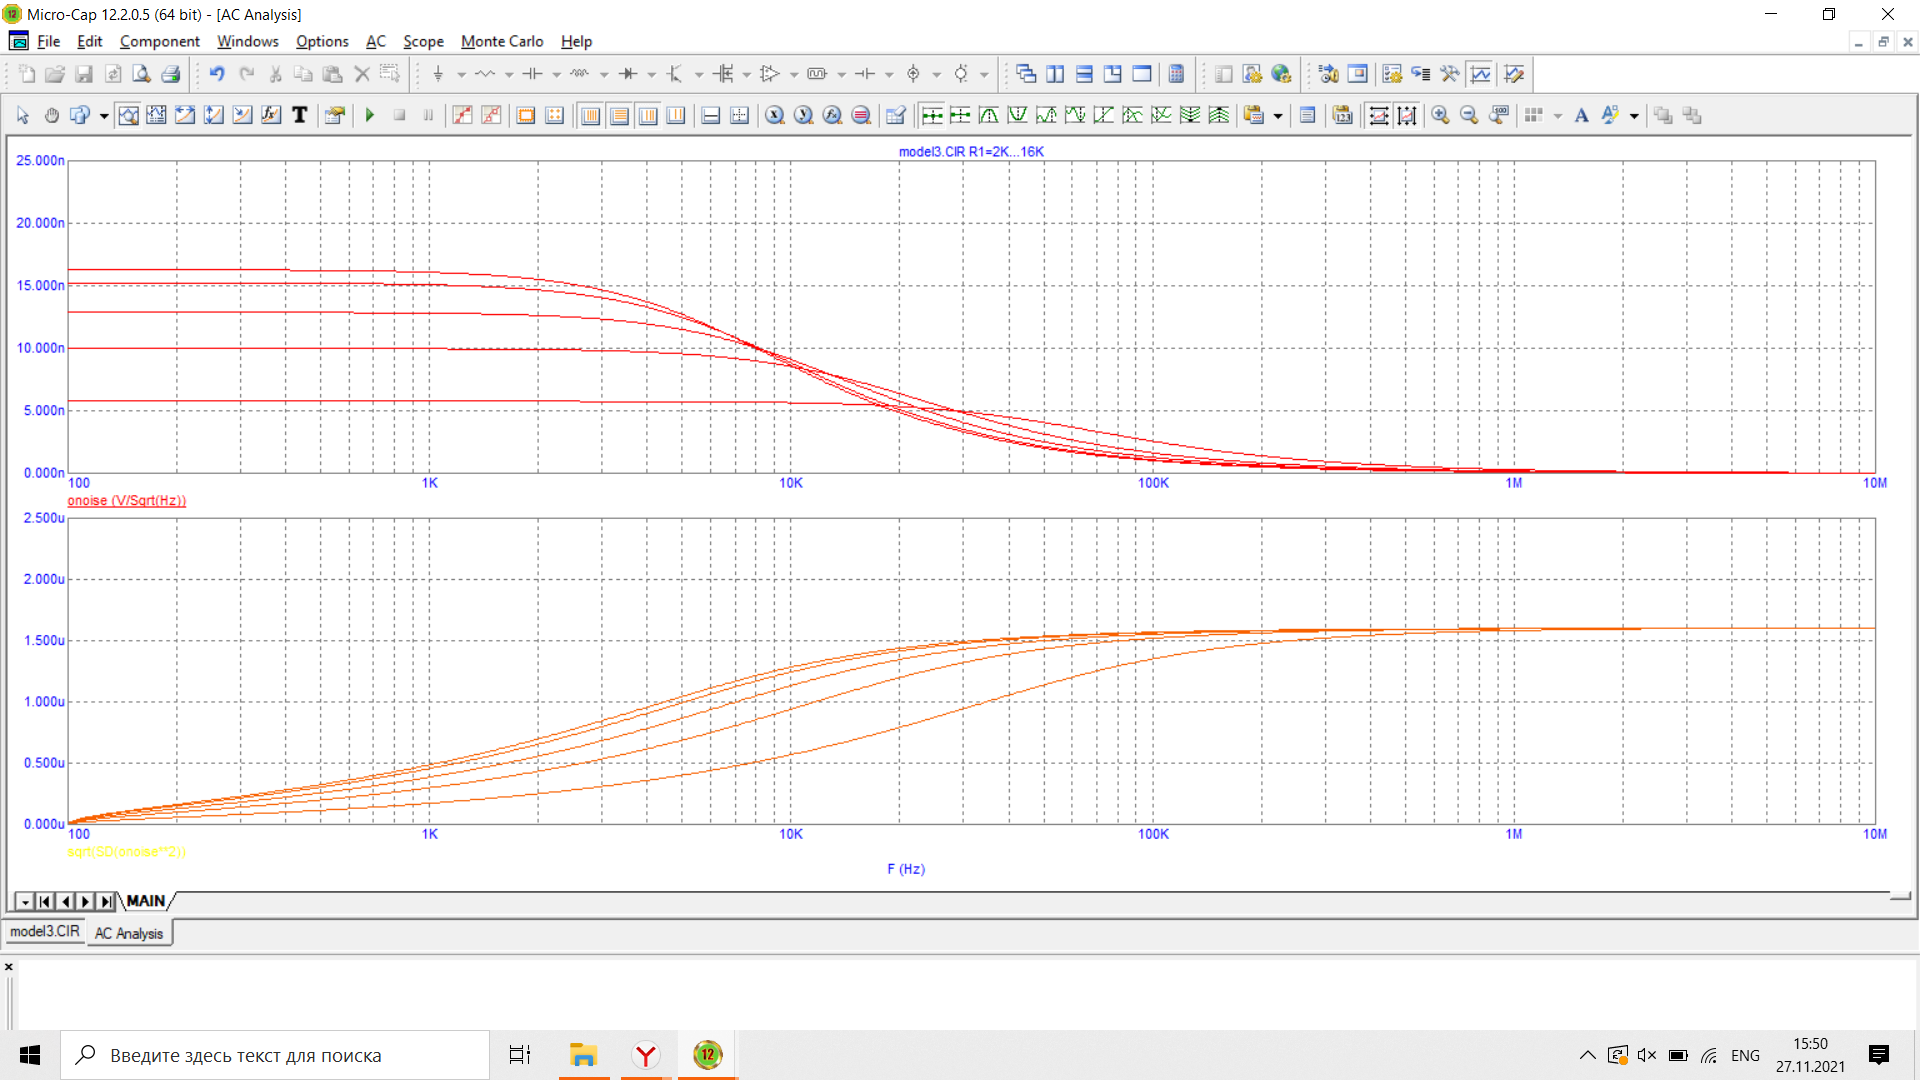
\includegraphics[scale = 0.4 \textwidth]{images/mod3_1_3.png}
    \caption{Варьирование $R_1$ = [2k, 16k|4k]}
    \label{fig:m313}
\end{figure}

Снимем зависимость уровня шума от $C_1$:
\begin{itemize}
    \item $C_1 = 0.8k => n_1(f) = 2.27\mu$;
    \item $C_1 = 1.2k => n_1(f) = 1.85\mu$;
    \item $C_1 = 1.6k => n_1(f) = 1.60\mu$;
    \item $C_1 = 2.0k => n_1(f) = 1.44\mu$;
    \item $C_1 = 2.4k => n_1(f) = 1.31\mu$;
\end{itemize}

\begin{figure}[h!]
    \centering
    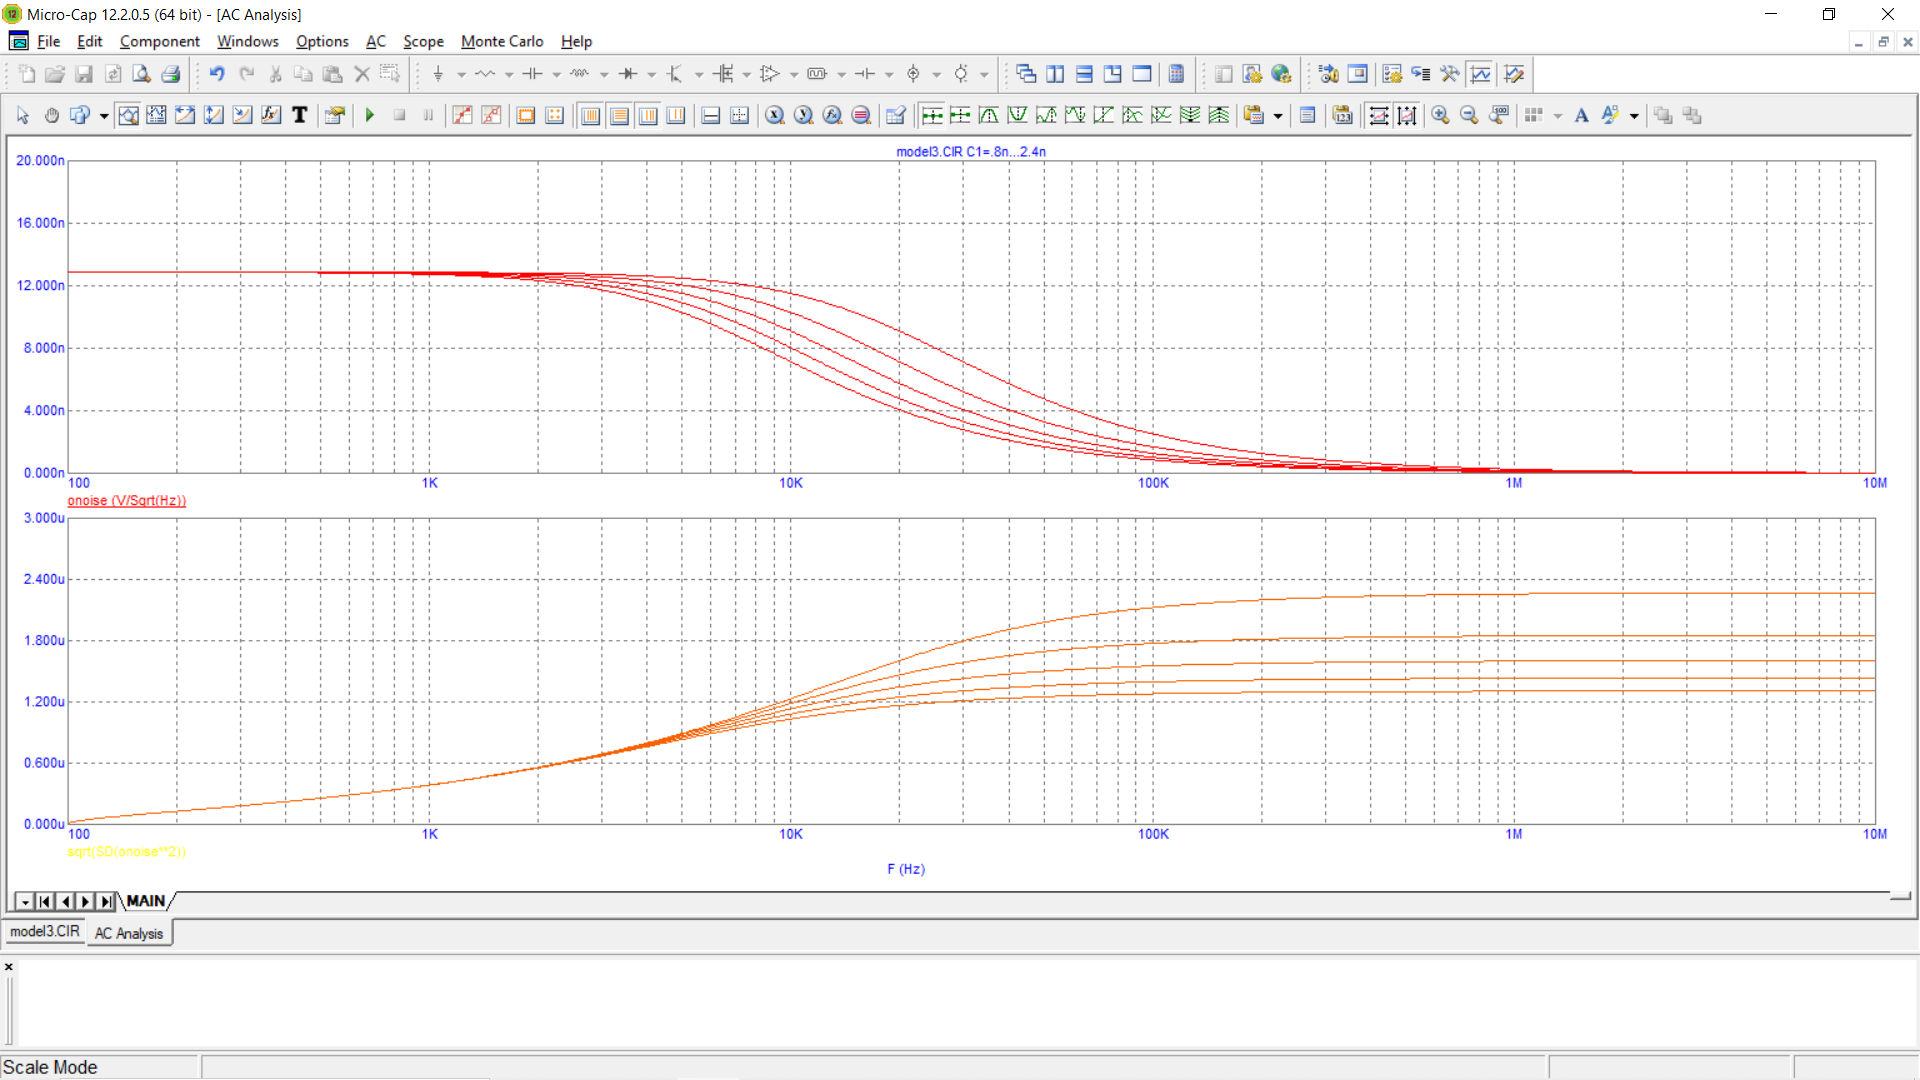
\includegraphics[scale = 0.4 \textwidth]{images/mod3_1_4.png}
    \caption{Варьирование $C_1$ = [0.8n, 2.4n|0.4n]}
    \label{fig:m314}
\end{figure}

\subsection{Полосовой LC-фильтр}

\begin{figure}[h!]
    \centering
    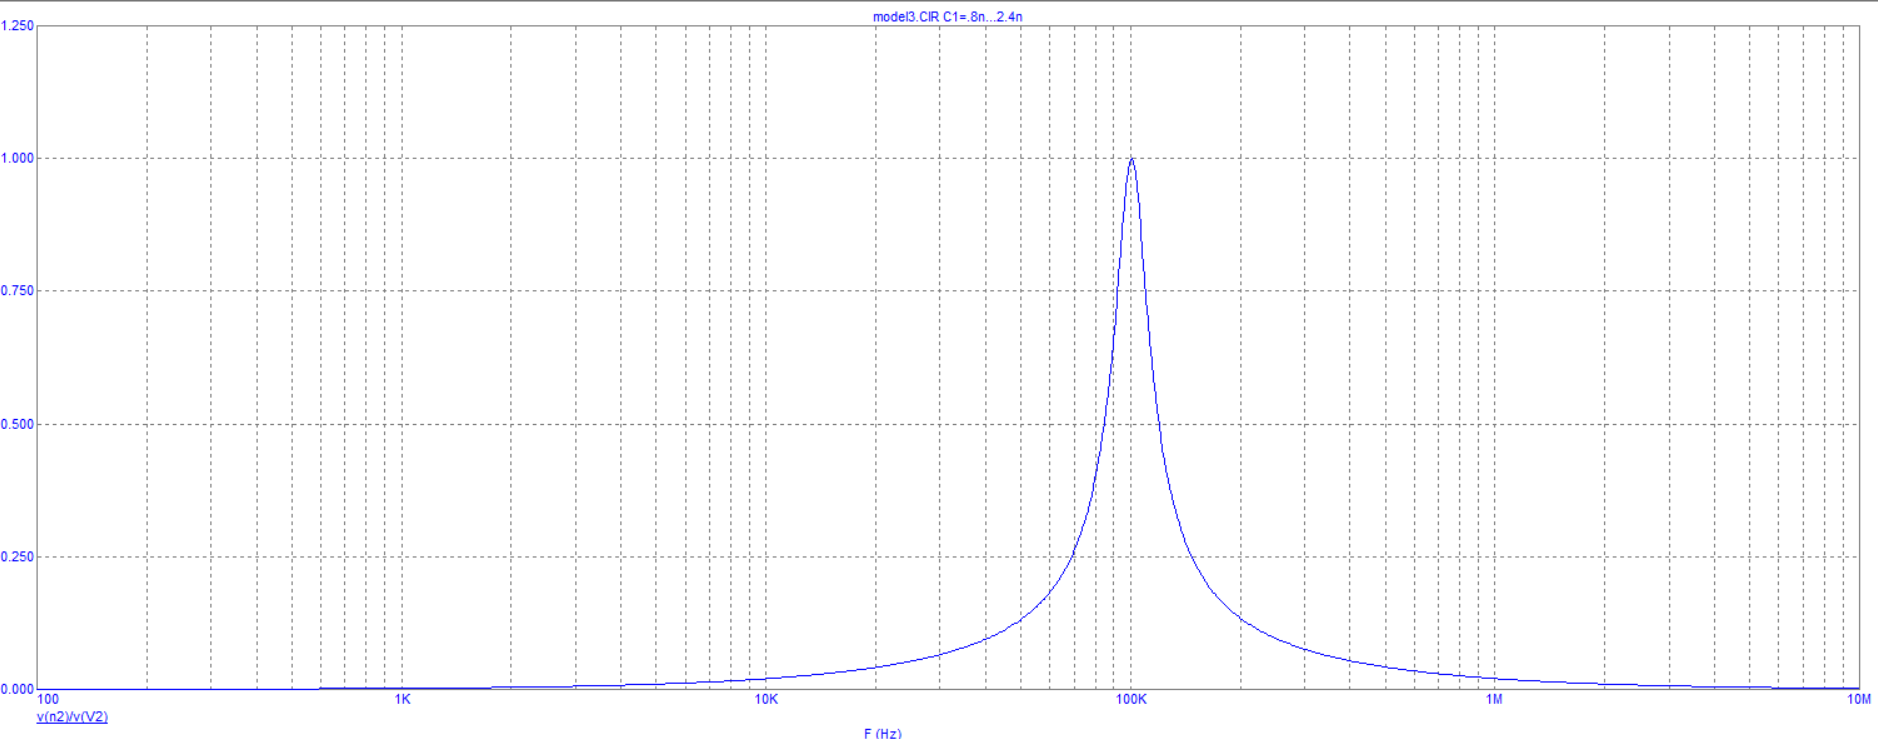
\includegraphics[scale = 0.4 \textwidth]{images/mod3_2_1.png}
    \caption{$f_0 = 100k, \Delta f = 20k$, Q = 5}
    \label{fig:m321}
\end{figure}

\begin{figure}[h!]
    \centering
    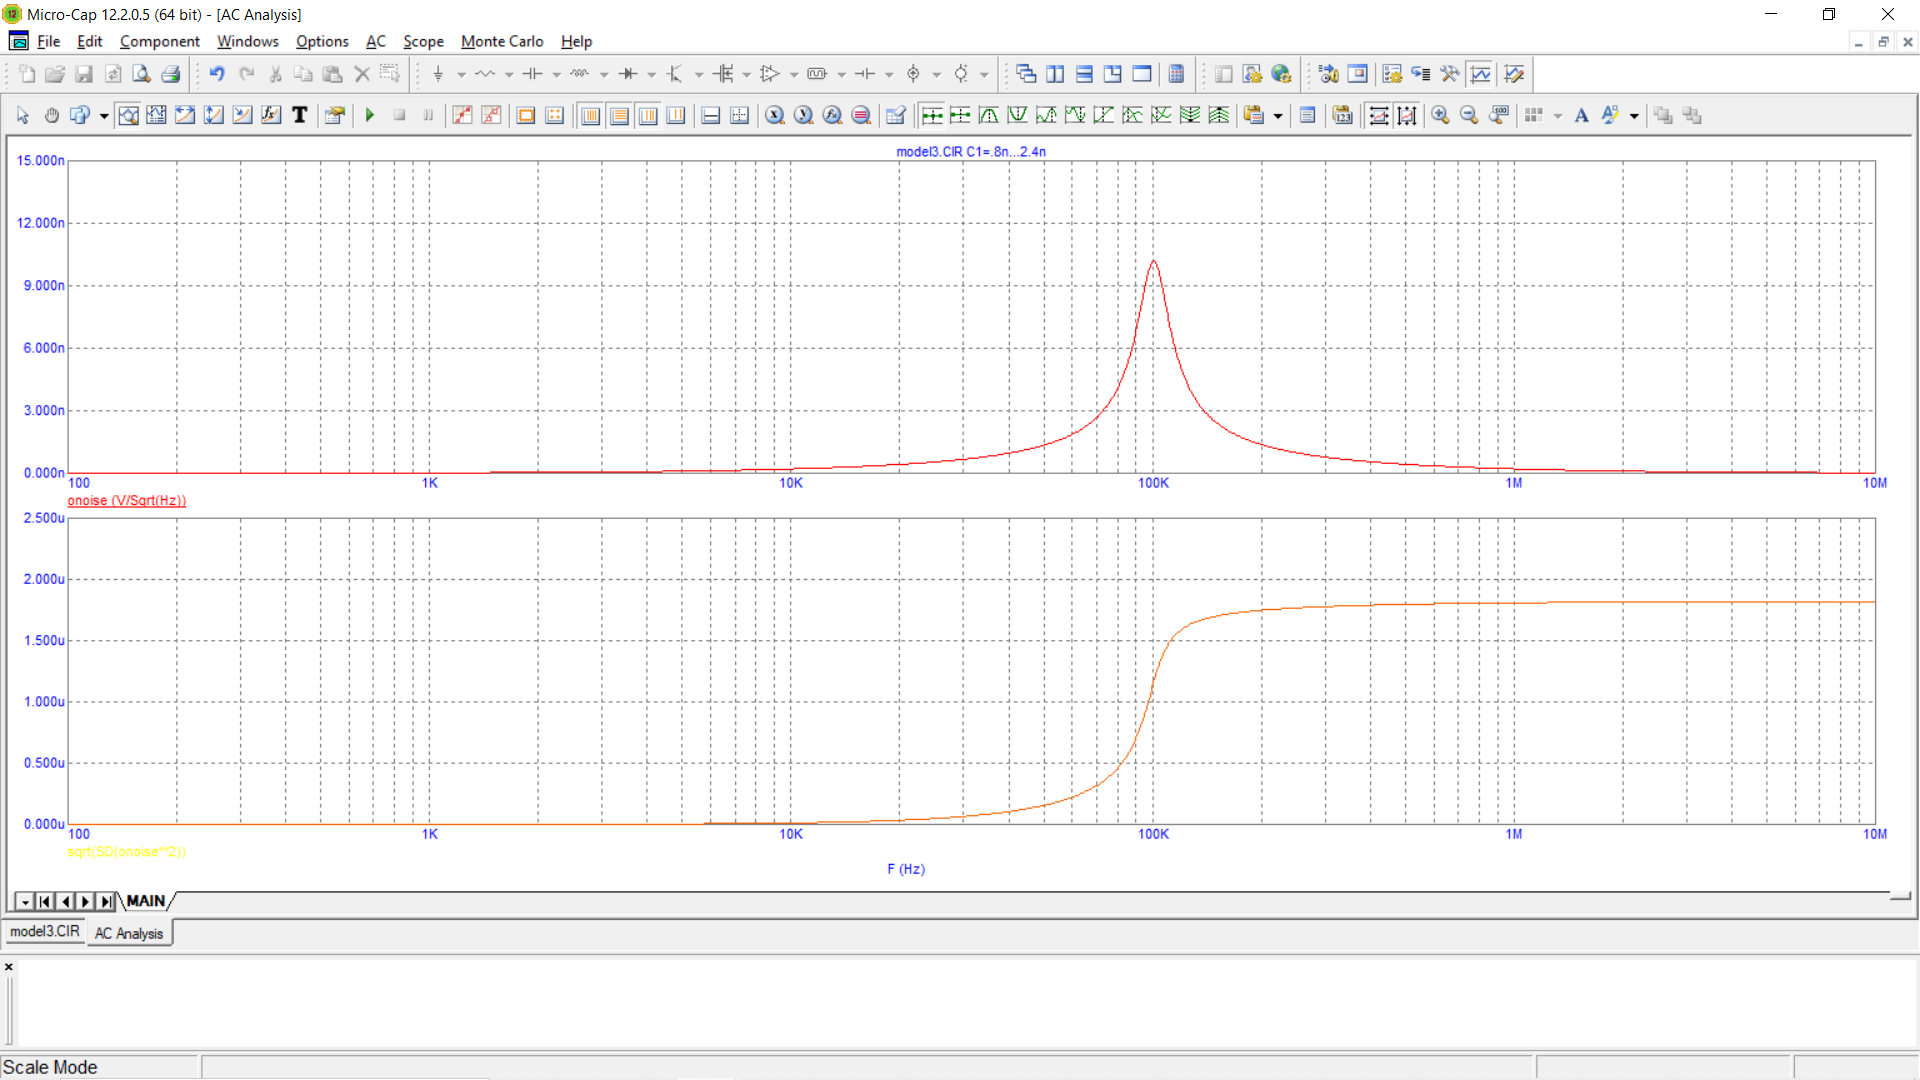
\includegraphics[scale = 0.4 \textwidth]{images/mod3_2_2.png}
    \caption{$n_2(f_0) = 10n, \sigma = 1.82\mu$}
    \label{fig:m322}
\end{figure}

Проверим формулу $\sigma = n_2\sqrt{F_n} = \sqrt{\frac{kT}{C}} = 1.80$, формула работает.

\begin{figure}[h!]
    \centering
    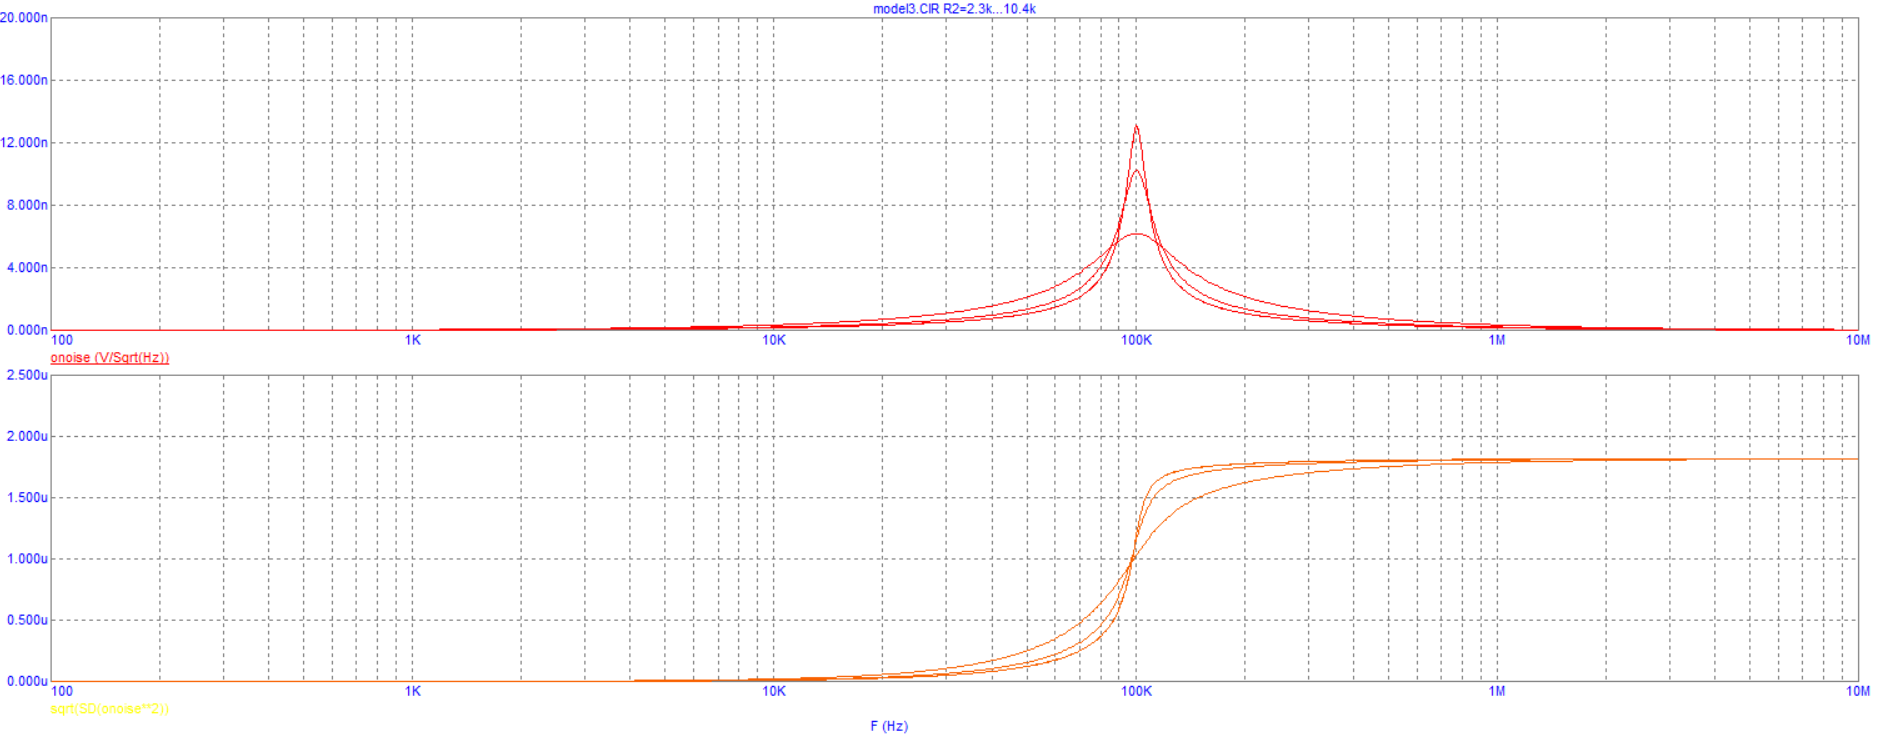
\includegraphics[scale = 0.4 \textwidth]{images/mod3_2_3.png}
    \caption{Варьирование $R_2$ = [2.3k, 10.3k|4k]}
    \label{fig:m323}
\end{figure}

Зависимость $n_2(f_0)$ от $R_2$:
\begin{itemize}
    \item $R_2 = 2.3k => n_2 = 6.08n$;
    \item $R_2 = 6.3k => n_2 = 10.08$;
    \item $R_2 = 10.3k => n_2 = 13.04$;
\end{itemize}

\begin{figure}[h!]
    \centering
    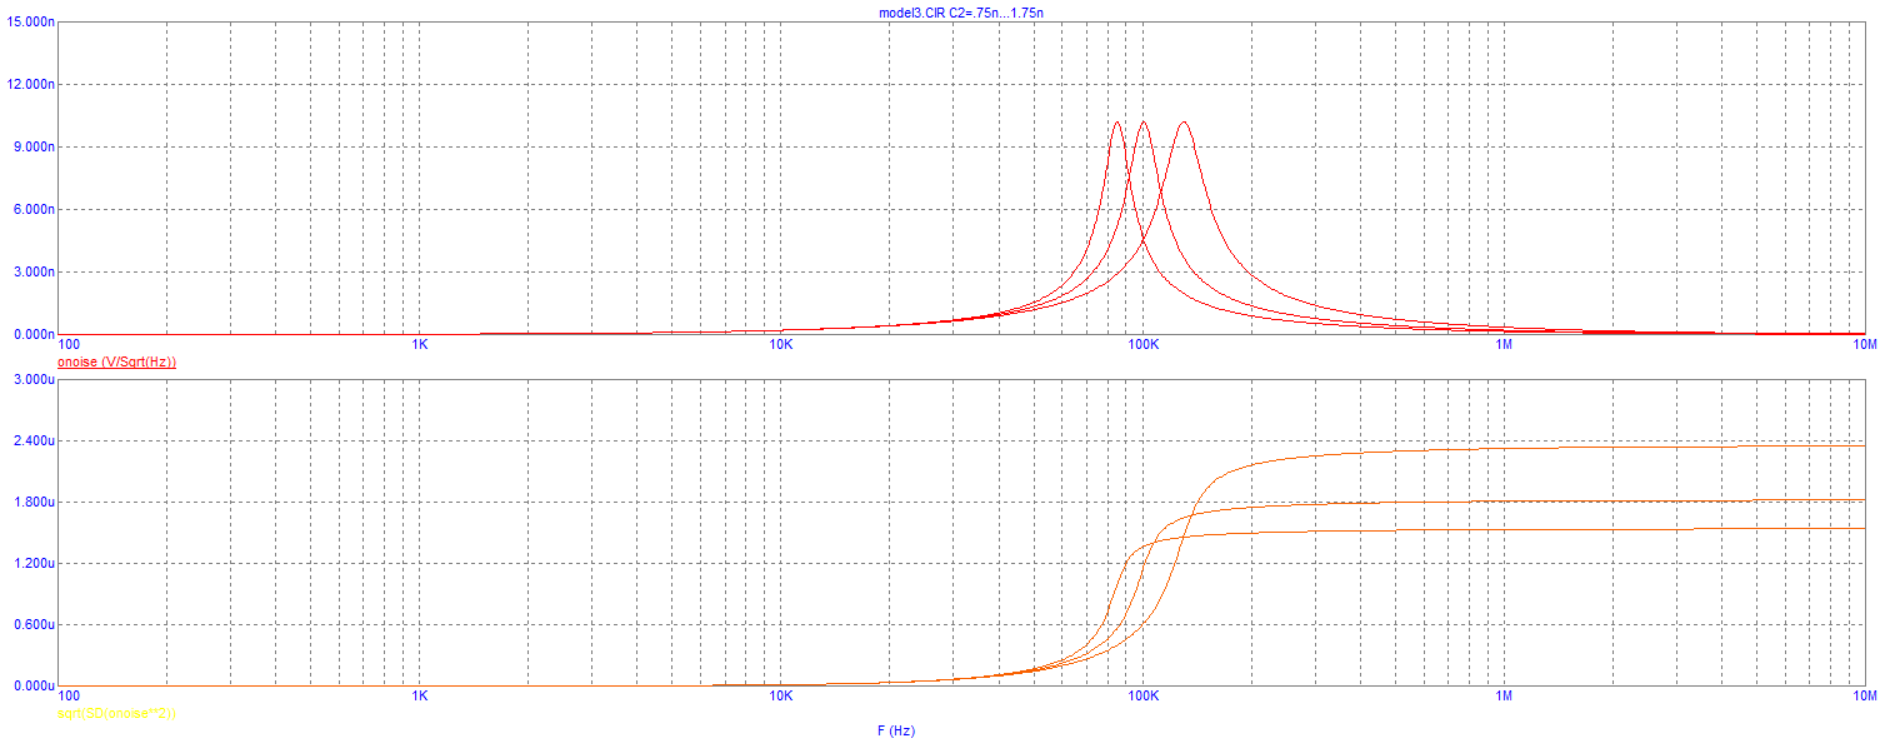
\includegraphics[scale = 0.4 \textwidth]{images/mod3_2_4.png}
    \caption{Варьирование $C_2$ = [0.75n, 1.75n|0.5n]}
    \label{fig:m324}
\end{figure}

Зависимость $\sigma$ от $C_2$:
\begin{itemize}
    \item $C_2 = 0.75n => \sigma = 2.34\mu$;
    \item $C_2 = 1.25n => \sigma = 1.82\mu$;
    \item $C_2 = 1.75n => \sigma = 1.52\mu$;
\end{itemize}

\begin{figure}[h!]
    \centering
    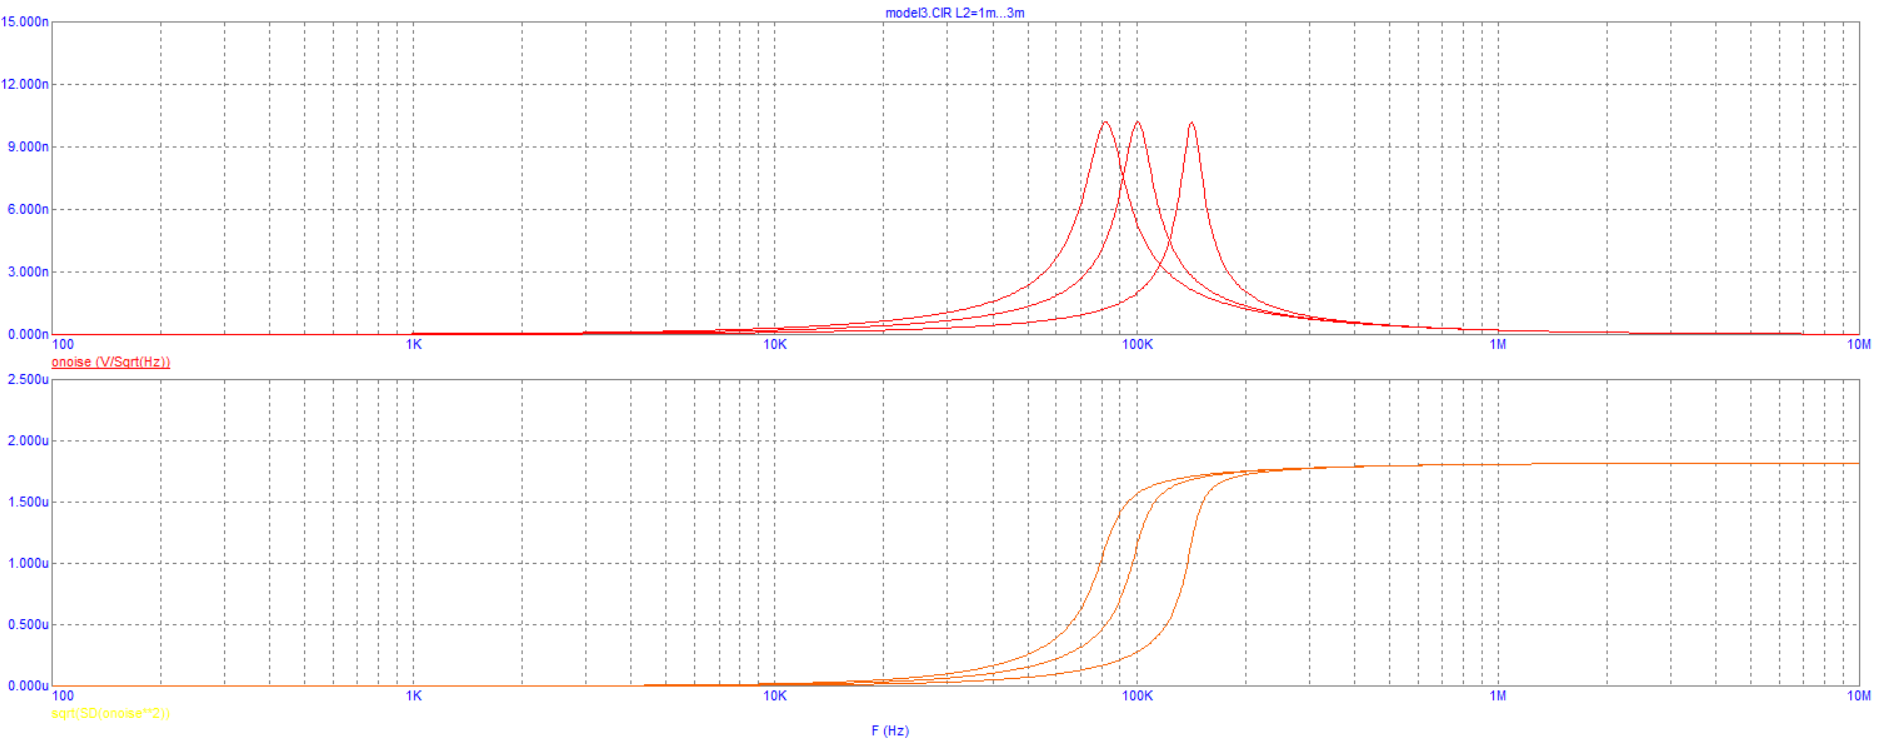
\includegraphics[scale = 0.4 \textwidth]{images/mod3_2_5.png}
    \caption{Варьирование $L_2$ = [1m, 3m|1m]}
    \label{fig:m325}
\end{figure}

\subsection{LC-фильтр нижних частот}

\begin{figure}[h!]
    \centering
    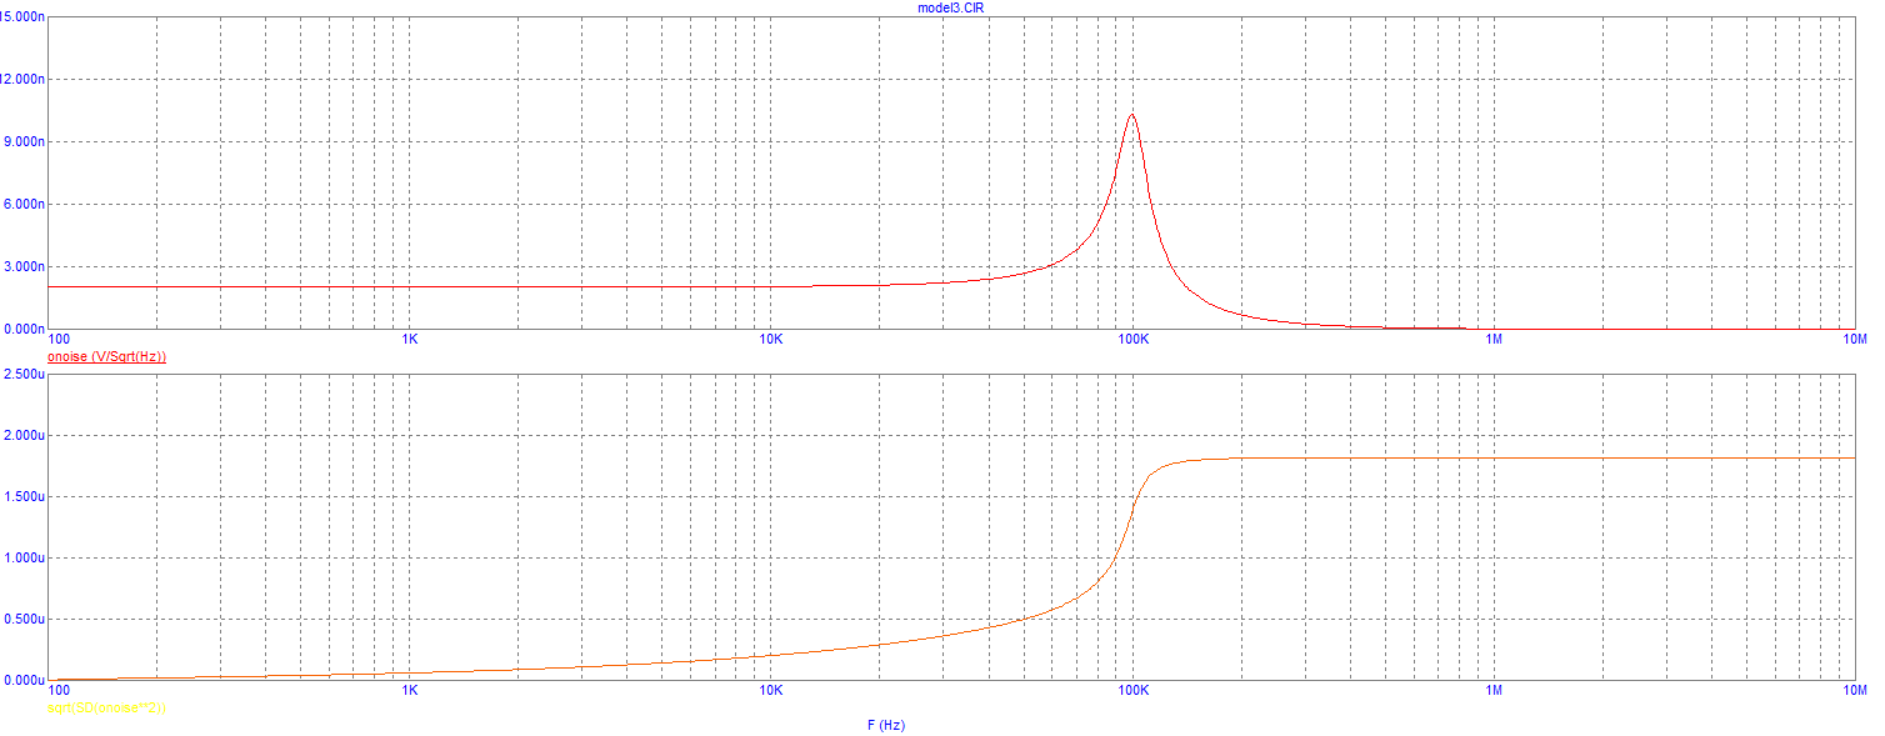
\includegraphics[scale = 0.4 \textwidth]{images/mod3_3_1.png}
    \caption{$n_3(f_0) = 10.2n, n_3(f_0/10) = 1.9n, \sigma = 1.82\mu$}
    \label{fig:m331}
\end{figure}

Оценим шумовую полосу $F_{n\text{теор}} = \frac{\pi}{2}\frac{f_0}{Q} = 31k, F_{n\text{прак}} = 30.9k$

\begin{figure}[h!]
    \centering
    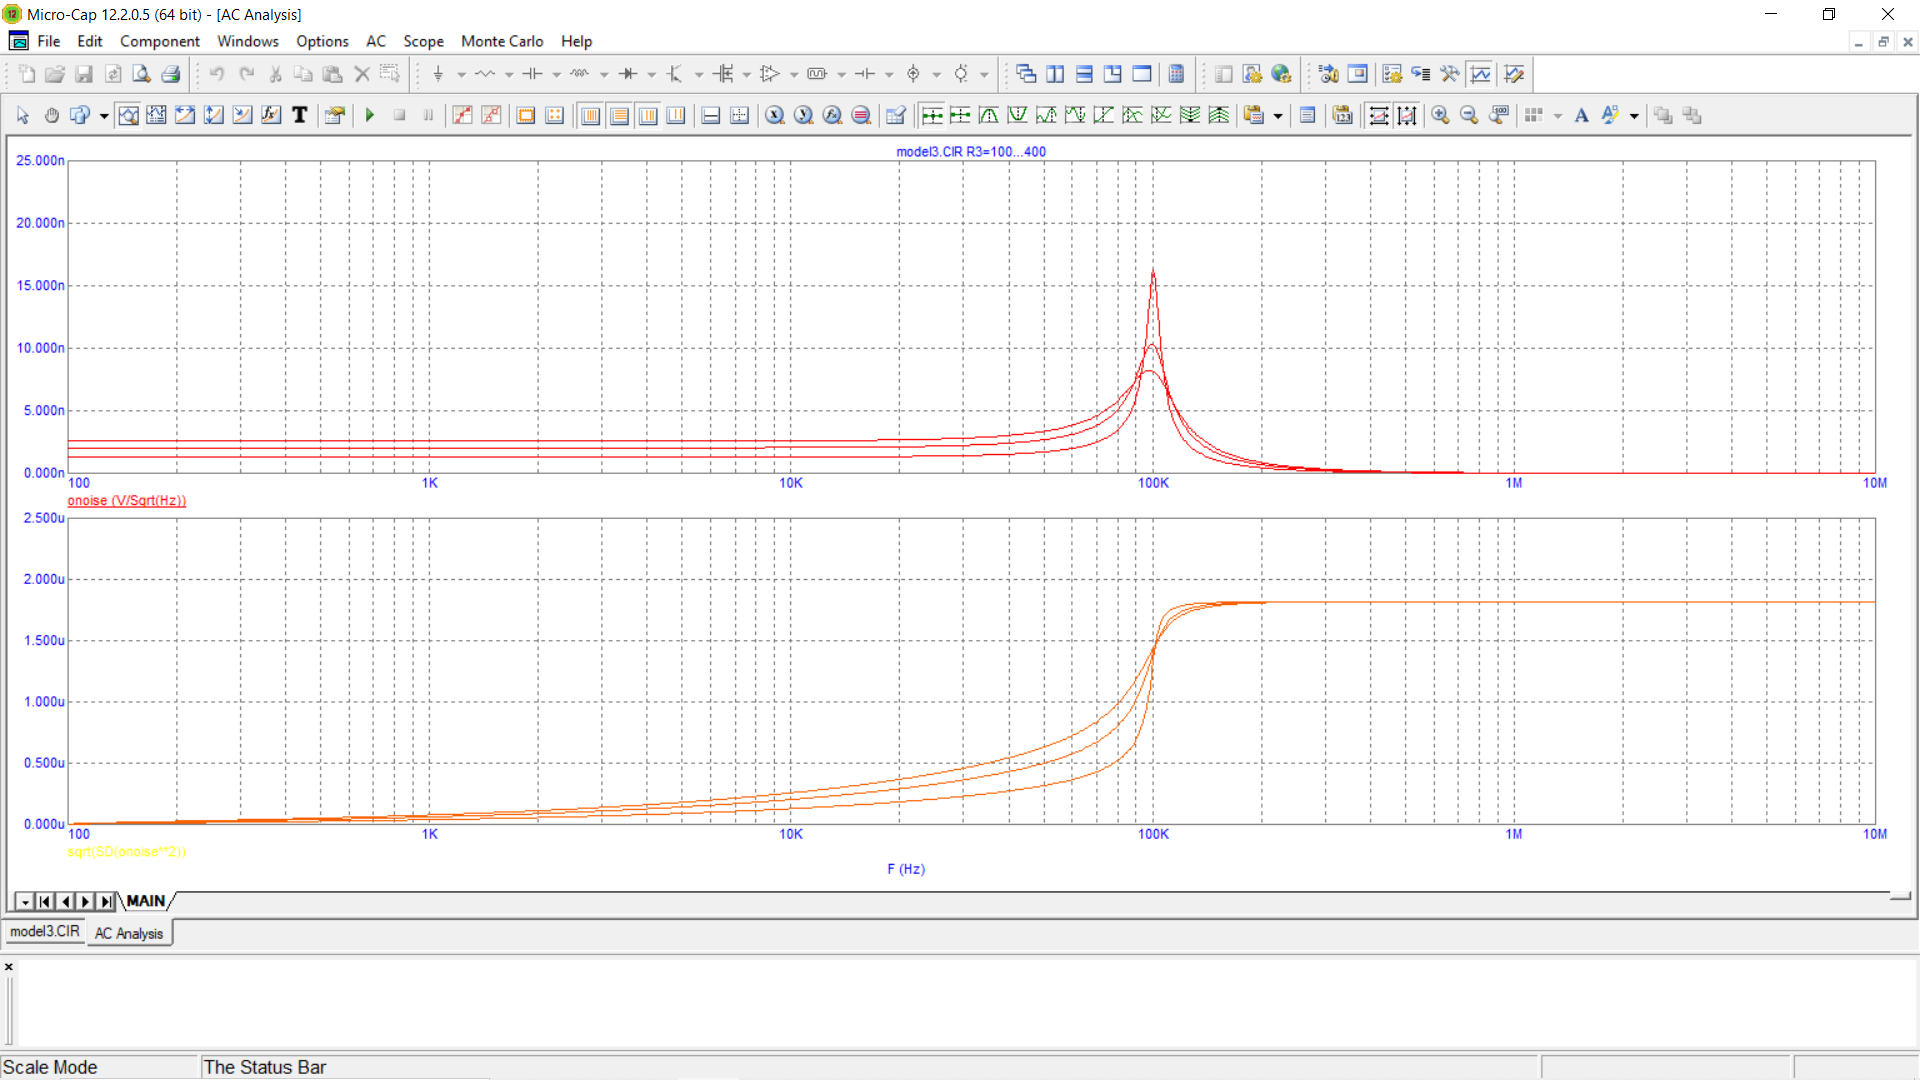
\includegraphics[scale = 0.4 \textwidth]{images/mod3_3_2_1.png}
    \caption{Варьирование R3 = [100,400|150]}
    \label{fig:m3321}
\end{figure}

\begin{tabular}{|c|c|c|c|}
    R3 & 400 & 250 & 100\\ \hline
    $n_3(f_0)$ & 8.1n & 10.3n & 15.9n\\ \hline
    $n_3(f_0/10)$ & 1.1n & 2n & 2.6n\\ \hline
    $\sigma$ & 1.8$\mu$ & &\\ \hline
\end{tabular}

\begin{figure}[h!]
    \centering
    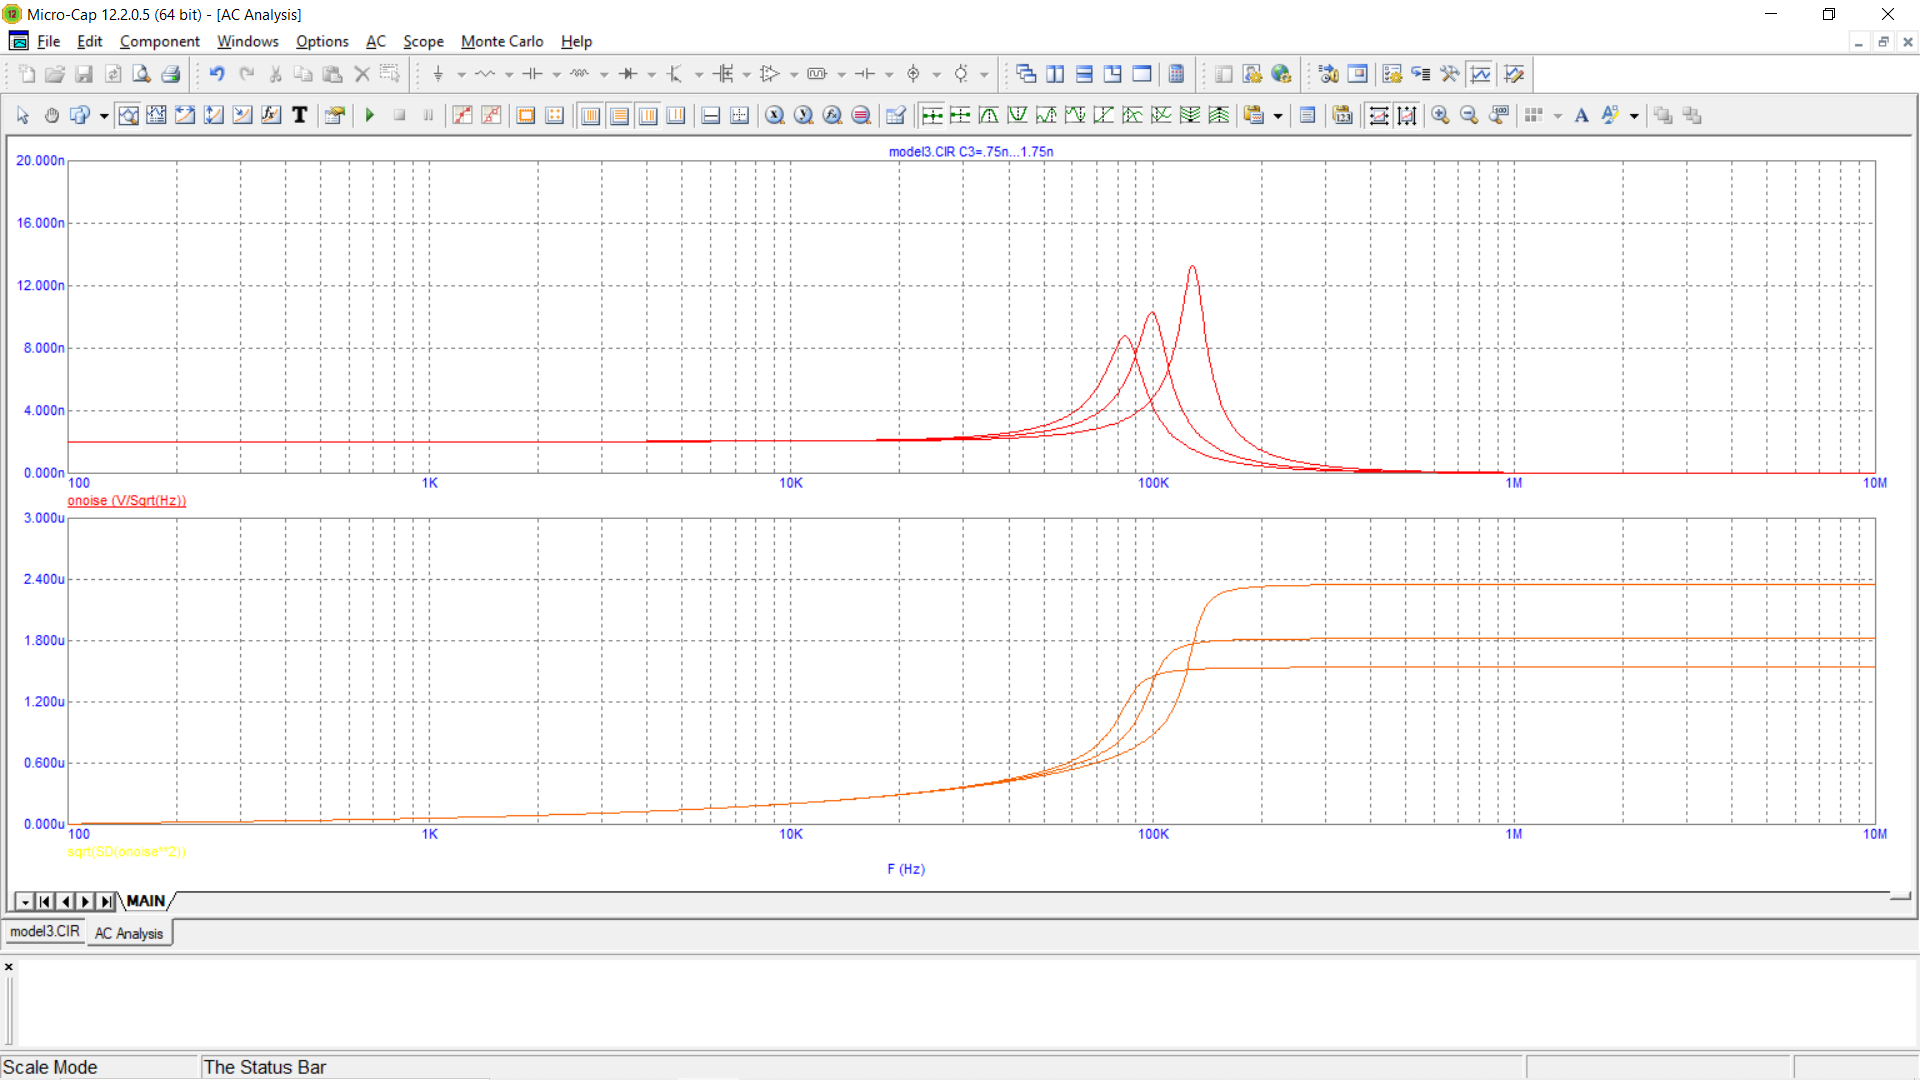
\includegraphics[scale = 0.4 \textwidth]{images/mod3_3_2_2.png}
    \caption{Варьирование C3 = [0.75n, 1.75n |0.5n]}
    \label{fig:m3322}
\end{figure}

\begin{tabular}{|c|c|c|c|}
    C3 & 0.75n & 1.25n & 1.75n\\ \hline
    $n_3(f_0)$ & 13.2n & 10.2n & 8.8n\\ \hline
    $n_3(f_0/10)$ & 2.1n &  & \\ \hline
    $\sigma$ & 2.4$\mu$ & 1.8$\mu$ & 1.5$\mu$ \\ \hline
\end{tabular}

\begin{figure}[h!]
    \centering
    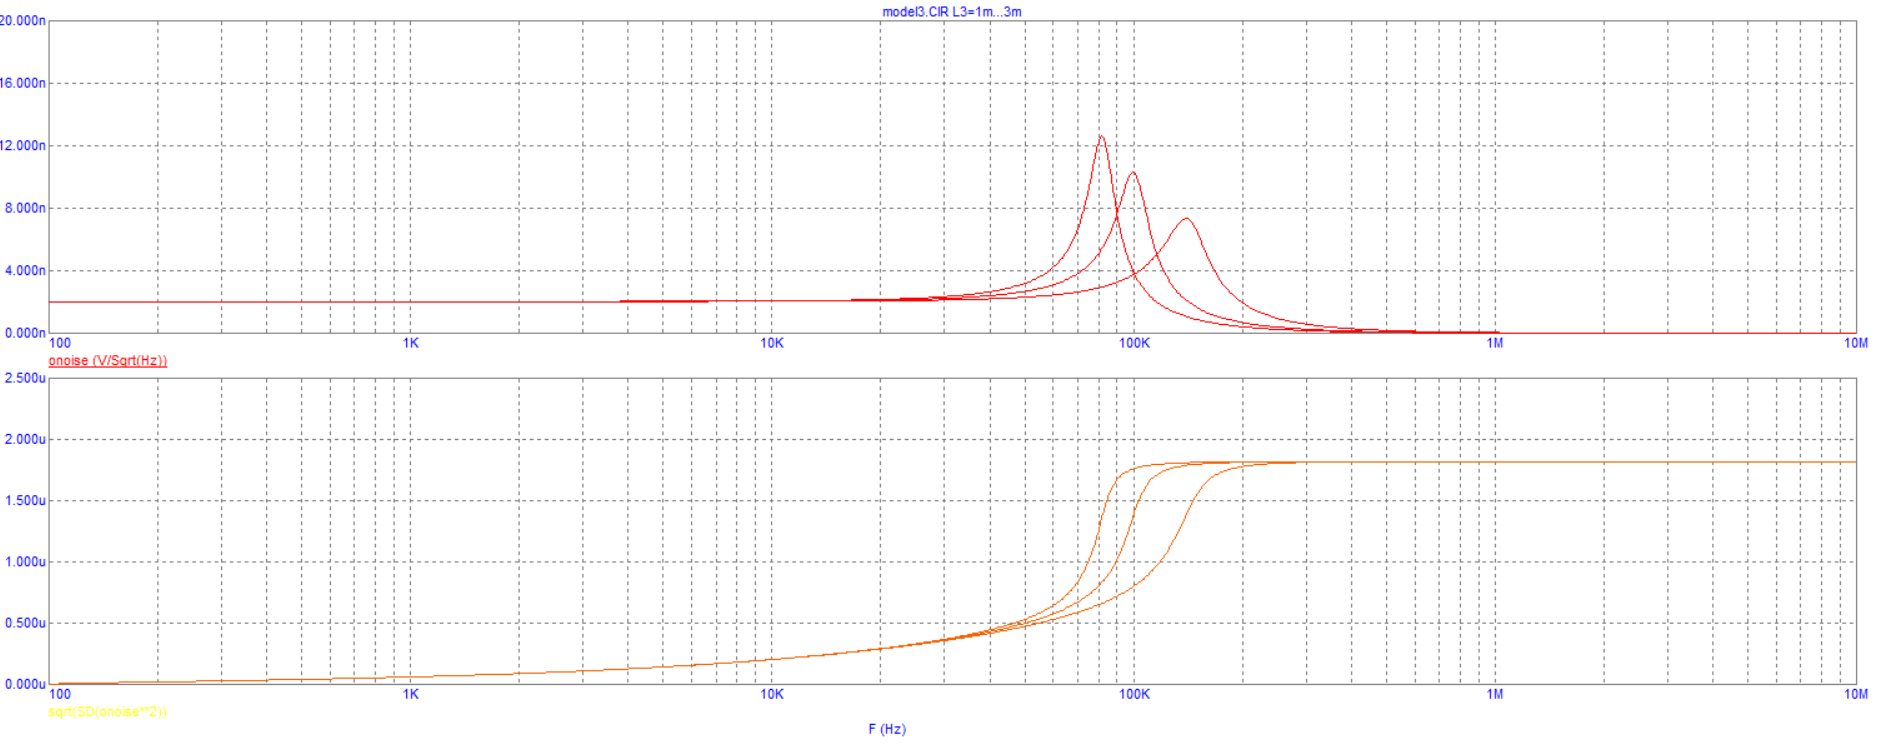
\includegraphics[scale = 0.4 \textwidth]{images/mod3_3_2_3.png}
    \caption{Варьирование L3 = [1m, 3m |1m]}
    \label{fig:m3323}
\end{figure}

\begin{tabular}{|c|c|c|c|}
    L3 & 1m & 2m & 3m\\ \hline
    $n_3(f_0)$ & 7.4n & 10.2n & 12.6n\\ \hline
    $n_3(f_0/10)$ & 2.1n &  & \\ \hline
    $\sigma$ & 1.8$\mu$ &  & \\ \hline
\end{tabular}

\subsection{LC-фильтр верхних частот}

\begin{figure}[h!]
    \centering
    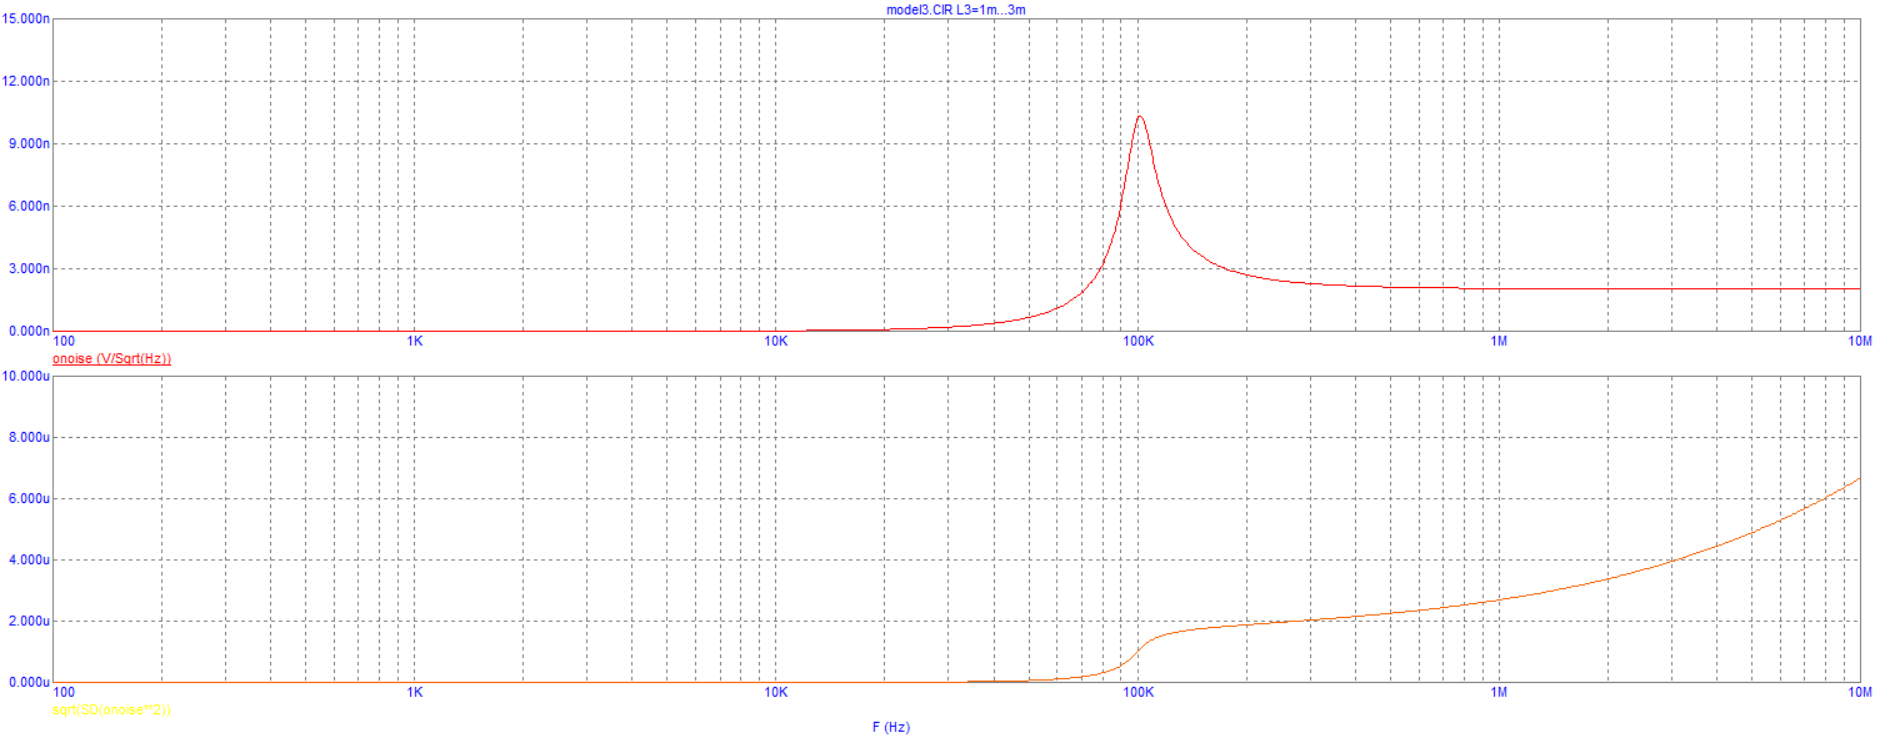
\includegraphics[scale = 0.4 \textwidth]{images/mod3_4_1.png}
    \caption{$n_4(f_0) = 10.3n, n_4(10 f_0) = 2.0n, \sigma = 2.7\mu$}
    \label{fig:m341}
\end{figure}

\begin{figure}[h!]
    \centering
    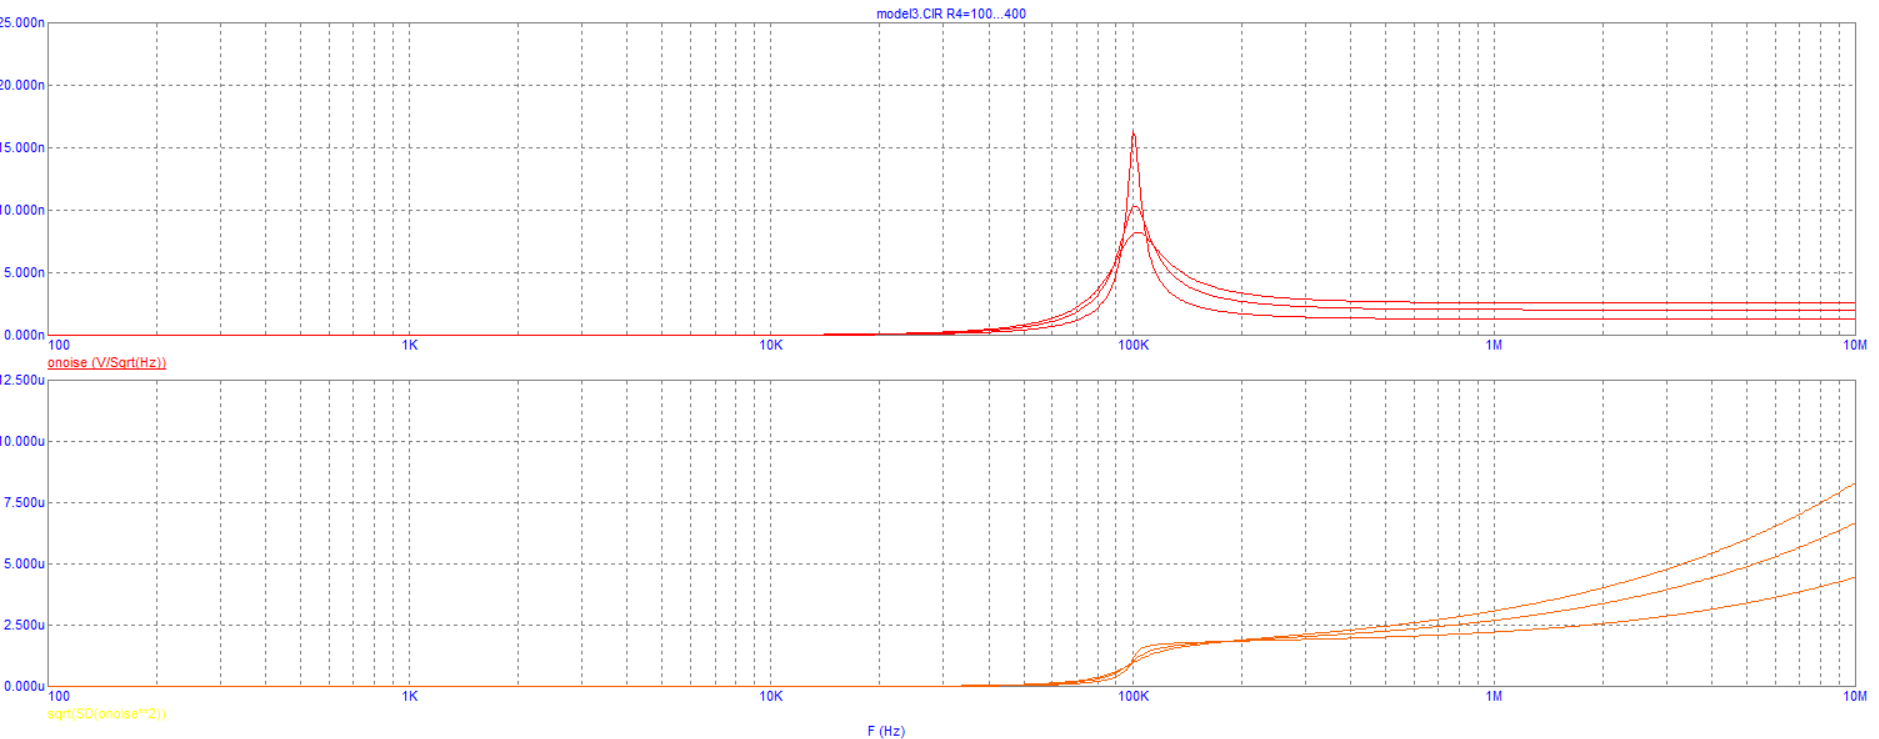
\includegraphics[scale = 0.4 \textwidth]{images/mod3_4_2_1.png}
    \caption{Варьирование R4 = [100,400|150]}
    \label{fig:m3421}
\end{figure}


\begin{tabular}{|c|c|c|c|}
    R3 & 400 & 250 & 100\\ \hline
    $n_4(f_0)$ & 8.2n & 10.2n & 15.9n\\ \hline
    $n_4(10 f_0)$ & 1.1n & 2n & 2.6n\\ \hline
    $\sigma$ & 3.0$\mu$ & 2.7$\mu$ & 2.2 $\mu$ \\ \hline
\end{tabular}

\begin{figure}[h!]
    \centering
    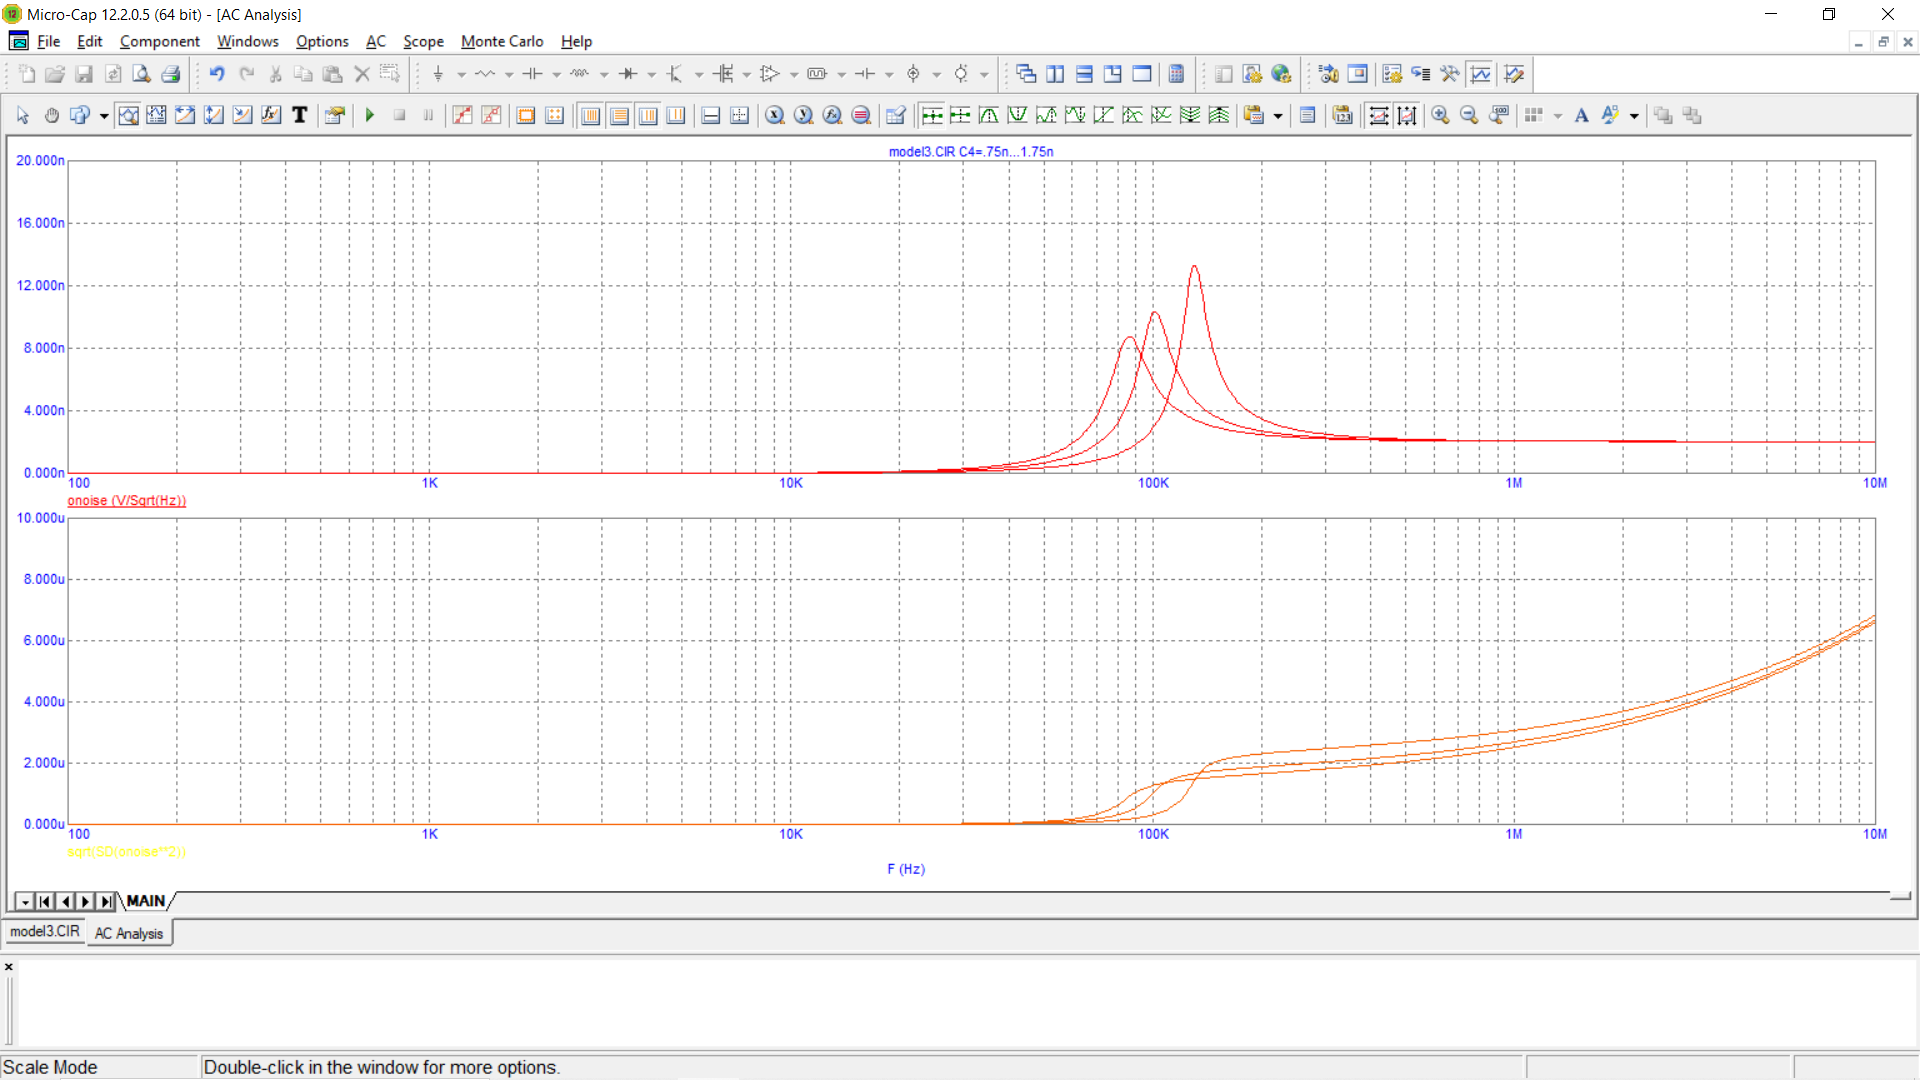
\includegraphics[scale = 0.4 \textwidth]{images/mod3_4_2_2.png}
    \caption{Варьирование C4 = [0.75n, 1.75n |0.5n]}
    \label{fig:m3422}
\end{figure}

\begin{tabular}{|c|c|c|c|}
    C4 & 0.75n & 1.25n & 1.75n\\ \hline
    $n_4(f_0)$ & 13.4n & 10.2n & 8.6n\\ \hline
    $n_4(10 f_0)$ & 1.9n &  & \\ \hline
    $\sigma$ & 3.1$\mu$ & 2.7$\mu$ & 2.5$\mu$\\ \hline
\end{tabular}

\begin{figure}[h!]
    \centering
    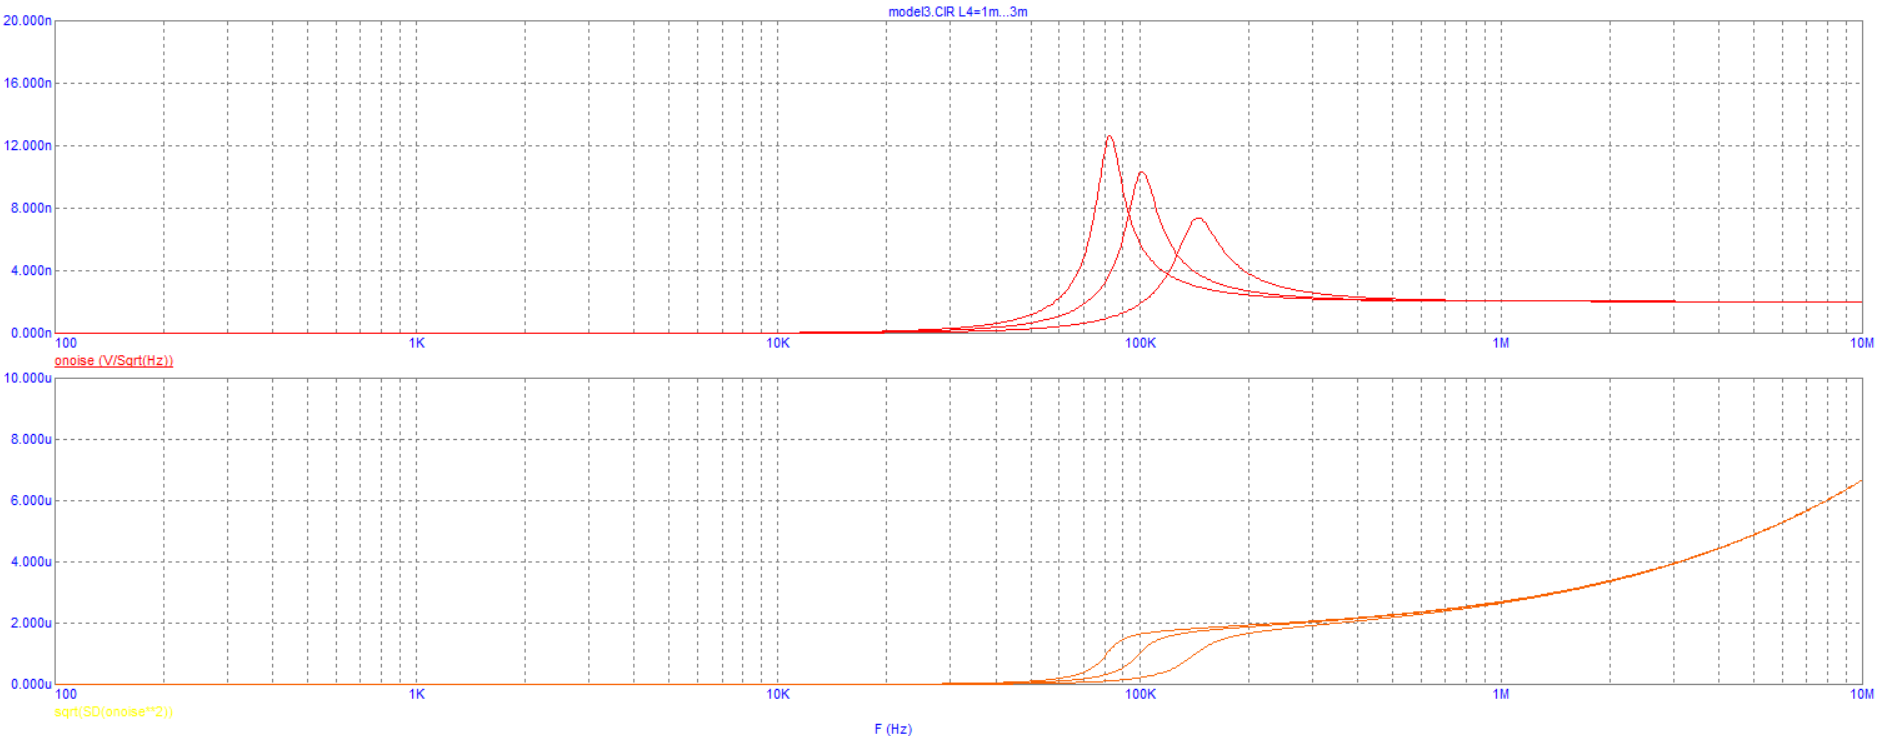
\includegraphics[scale = 0.4 \textwidth]{images/mod3_4_2_3.png}
    \caption{Варьирование L4 = [1m, 3m |1m]}
    \label{fig:m3423}
\end{figure}

\begin{tabular}{|c|c|c|c|}
    L3 & 1m & 2m & 3m\\ \hline
    $n_4(f_0)$ & 7.4n & 10.4n & 12.6n\\ \hline
    $n_4(10 f_0)$ & 2.0n &  & \\ \hline
    $\sigma$ & 2.6$\mu$ &  & \\ \hline
\end{tabular}

\section{\textbf{model4}}

\subsection{Полосовой LC-фильтр}
\FloatBarrier
\begin{figure}[h!]
    \centering
    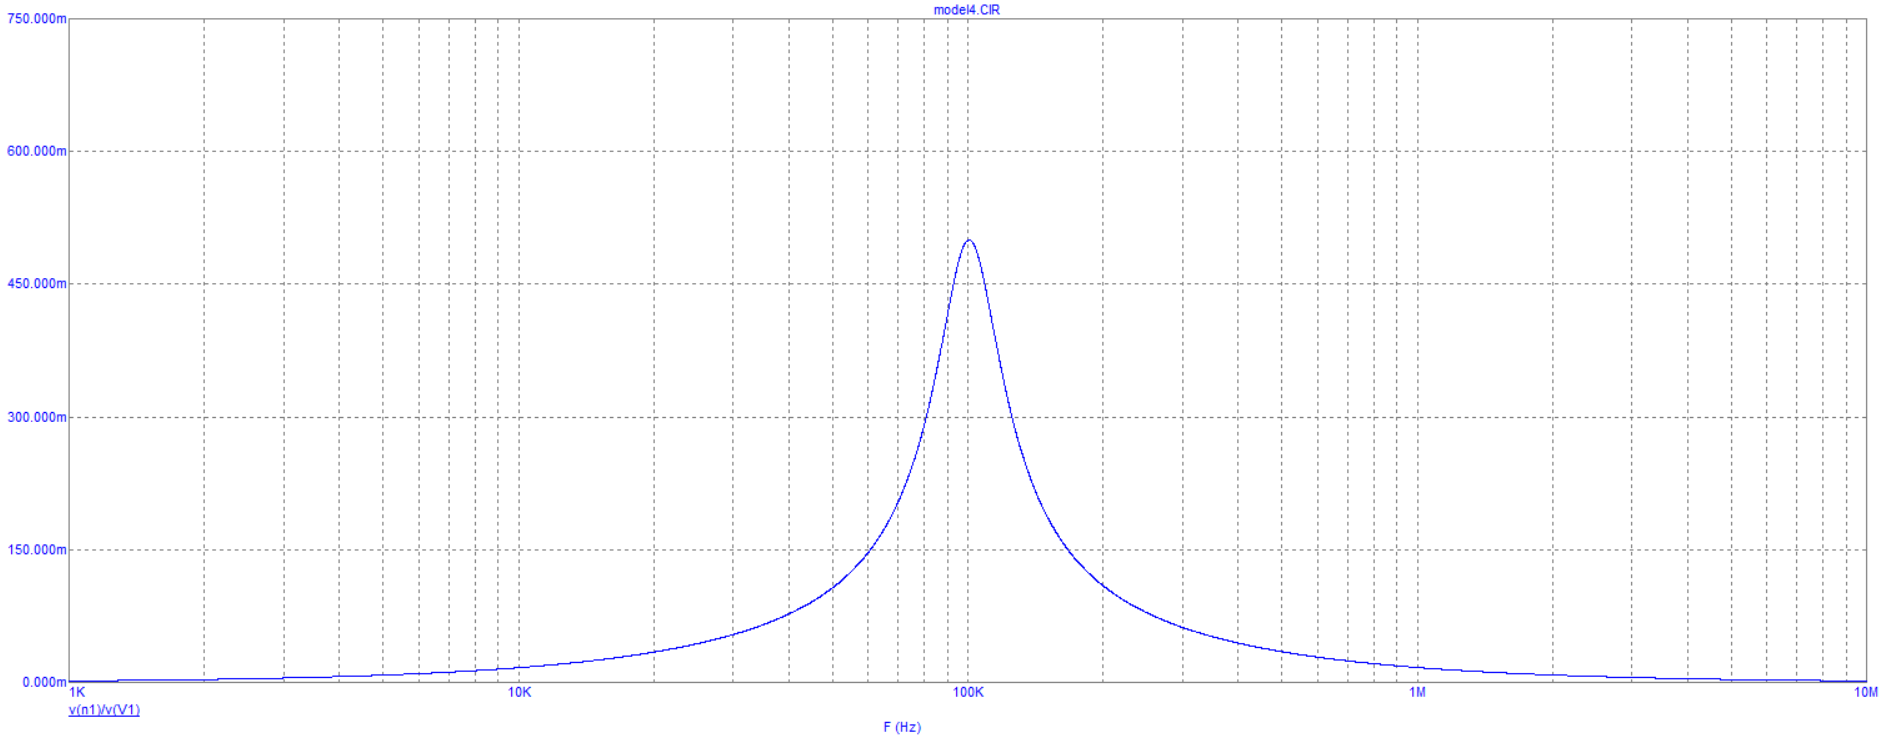
\includegraphics[scale = 0.4 \textwidth]{images/mod4_1_1.png}
    \caption{$f_0 = 100K, F = 32K, K = 0.5$, с теорией соотносится}
    \label{fig:m411}
\end{figure}

\begin{figure}[h!]
    \centering
    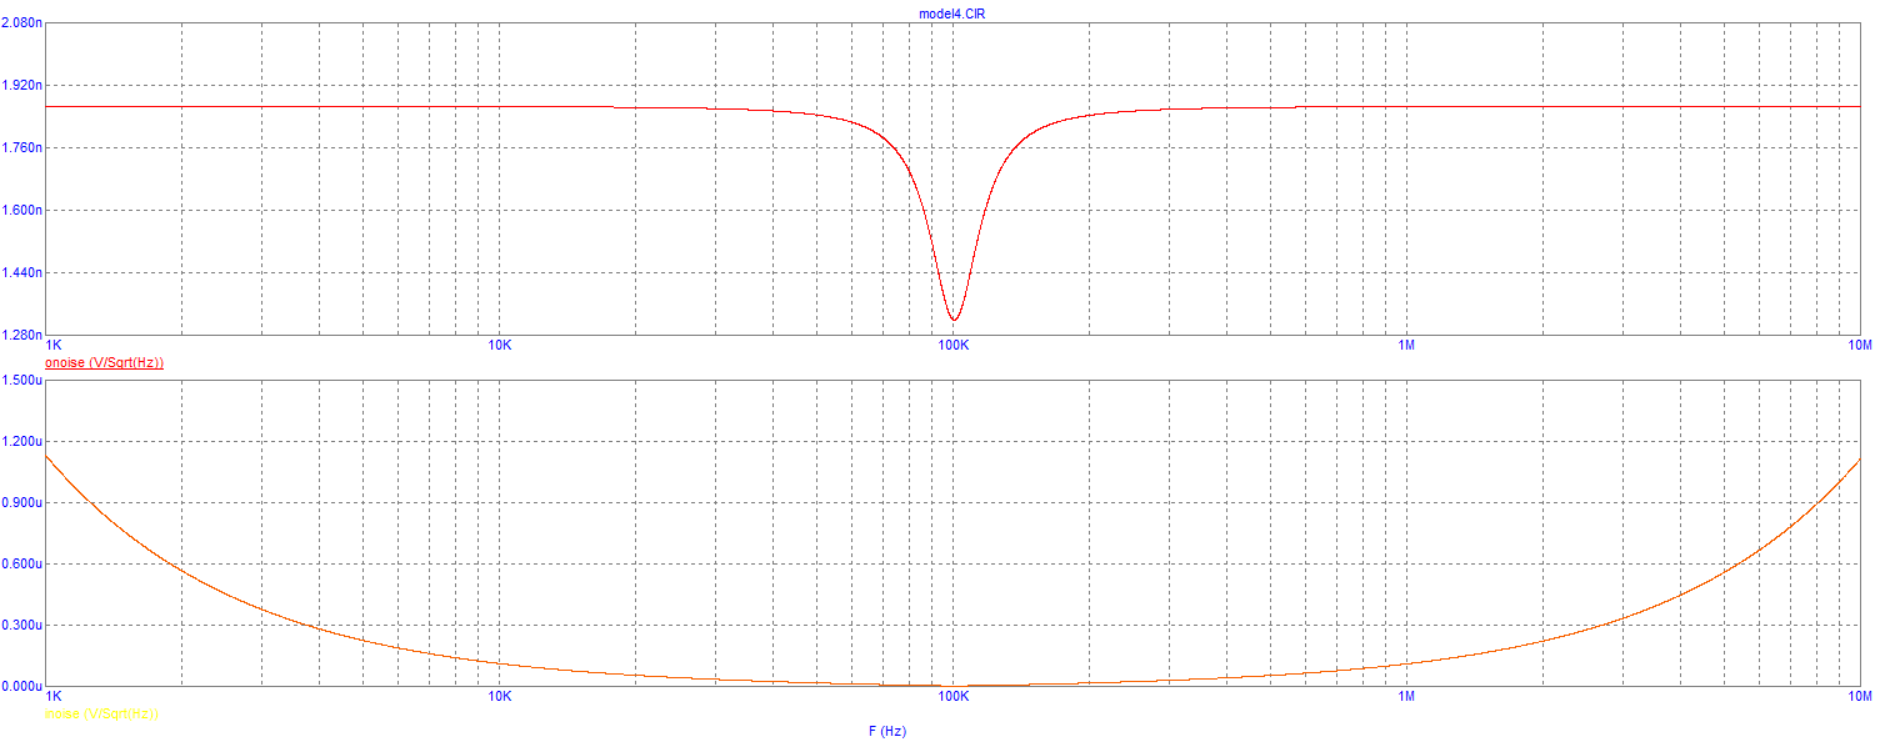
\includegraphics[scale = 0.4 \textwidth]{images/mod4_1_2_1.png}
    \caption{$n(f_0) = 1.32n, n(f_0/10) = 1.89n, \sigma = 1.82\mu$, оба резистора шумящие}
    \label{fig:m4121}
\end{figure}

\begin{figure}[h!]
    \centering
    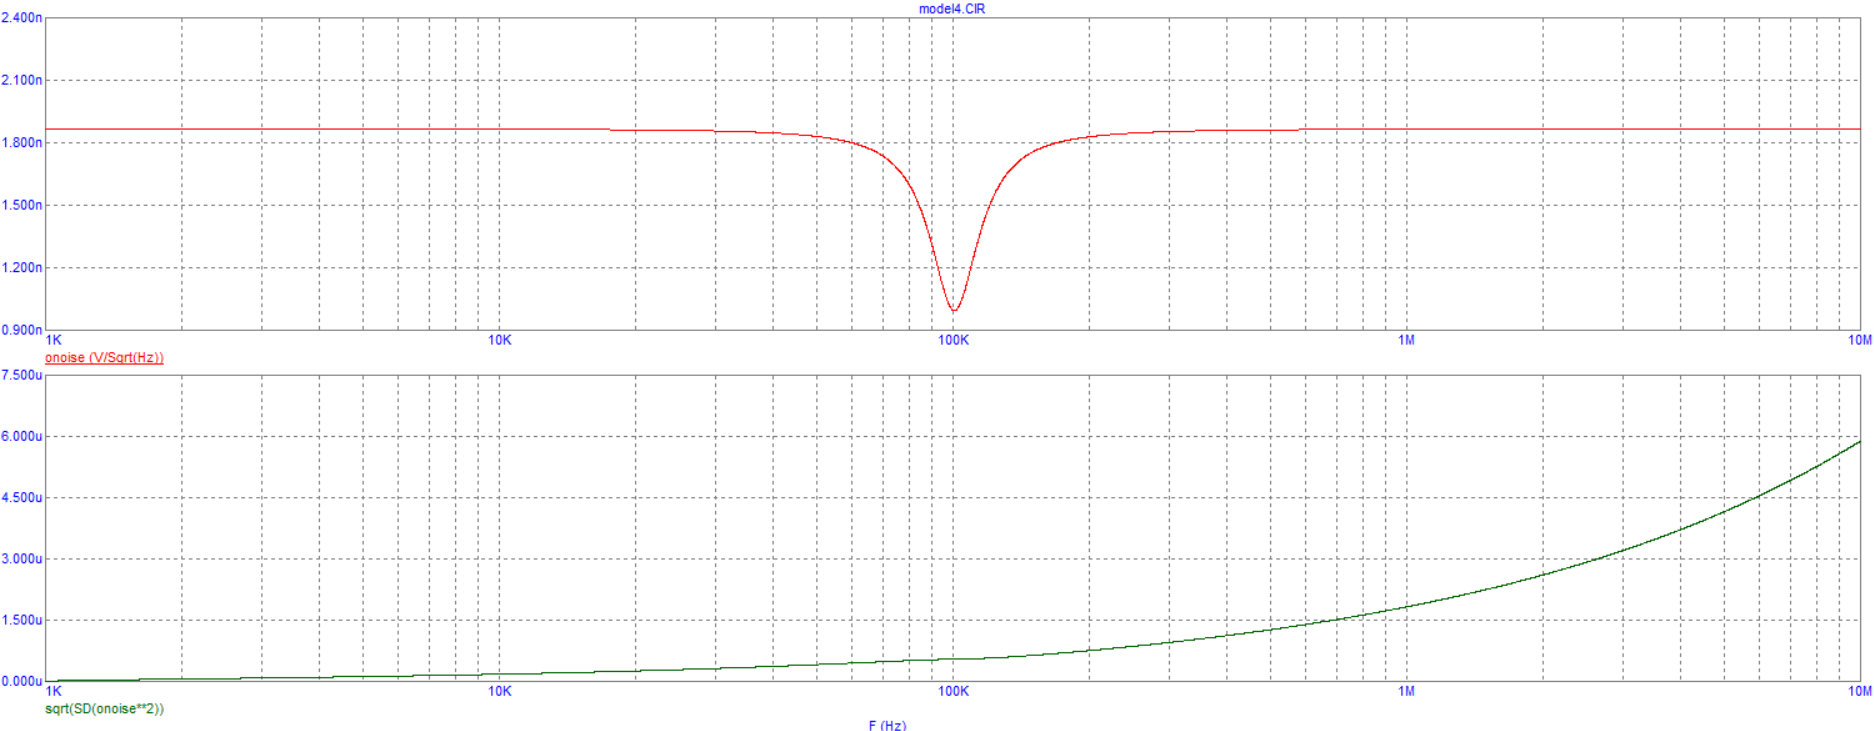
\includegraphics[scale = 0.4 \textwidth]{images/mod4_1_2_2.png}
    \caption{$n(f_0) = 1.01n, n(f_0/10) = 1.86n, \sigma = 5.9 \mu$, $R_s1$ - не шумящий}
    \label{fig:m4122}
\end{figure}

\begin{figure}[h!]
    \centering
    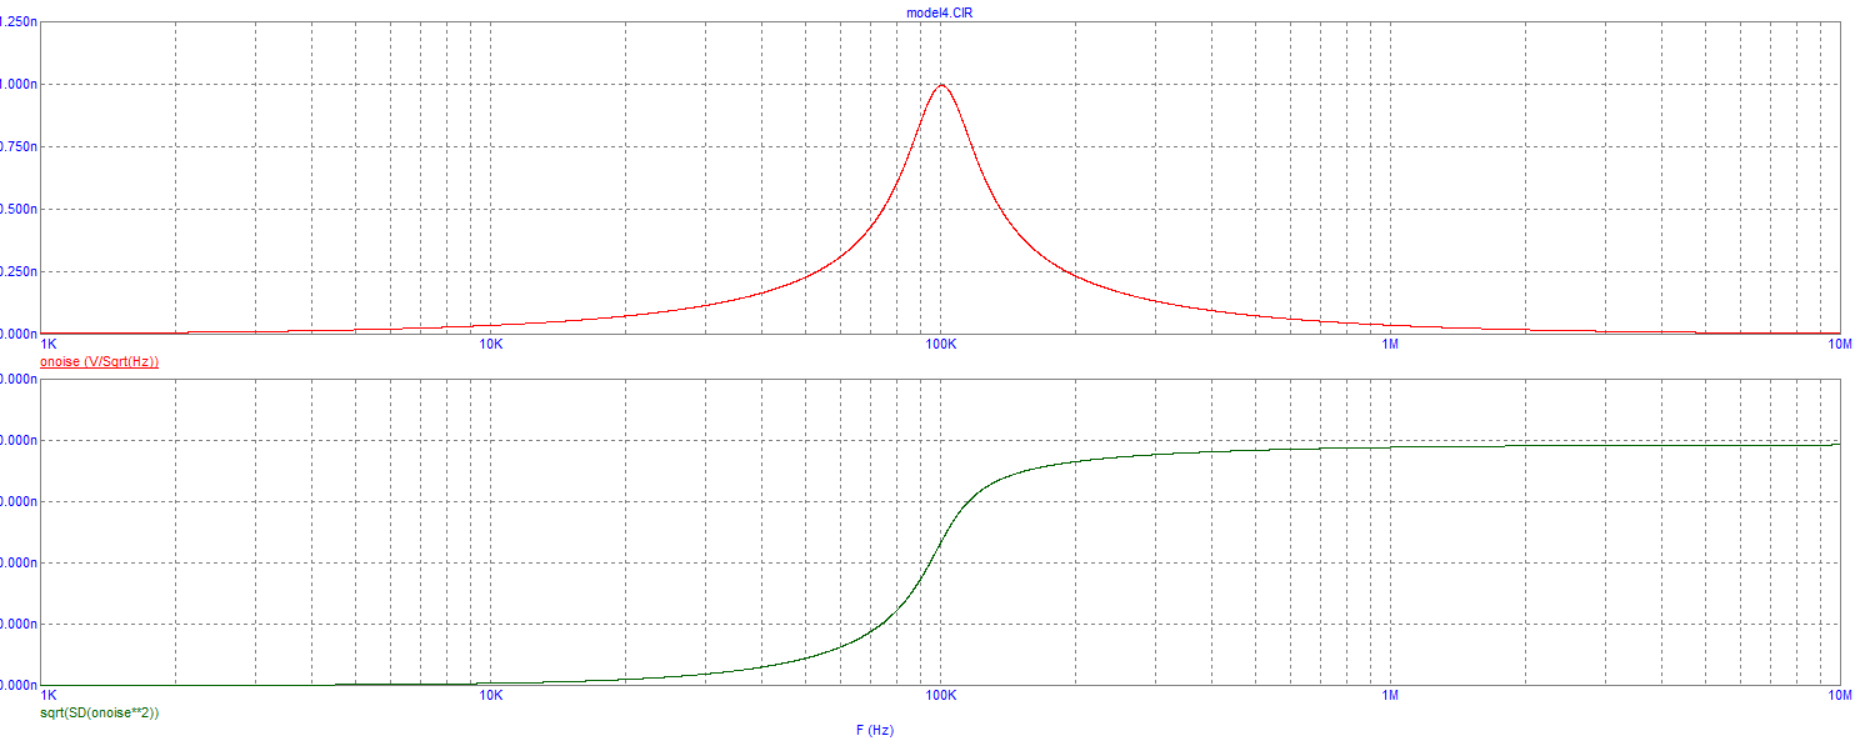
\includegraphics[scale = 0.4 \textwidth]{images/mod4_1_2_3.png}
    \caption{$n(f_0) = 1.01n, n(f_0/10) = 30p, \sigma = 240n$, $R_1$ - не шумящий}
    \label{fig:m4122}
\end{figure}

\begin{figure}[h!]
    \centering
    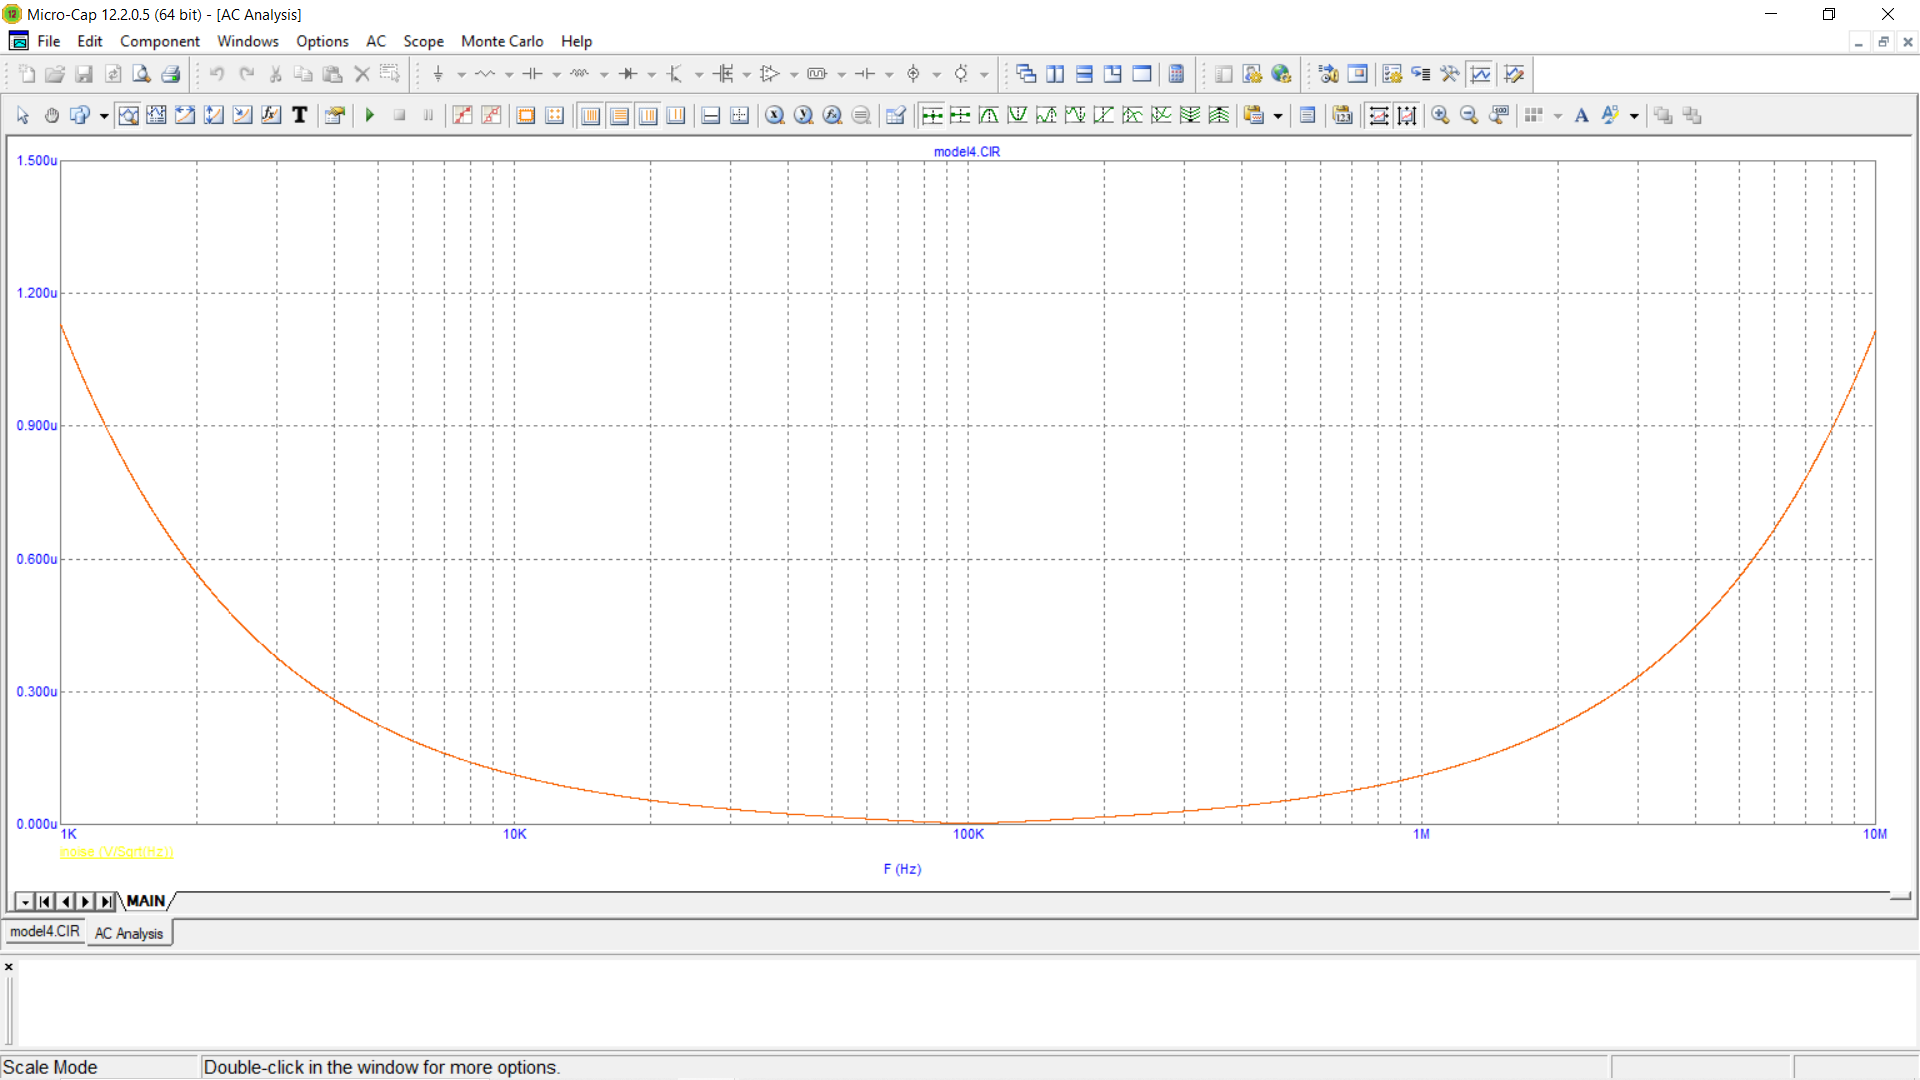
\includegraphics[scale = 0.4 \textwidth]{images/mod4_1_3.png}
    \caption{$e(f_0) = 2.6n, e(f_0/10) = 110.1n => K_n(f_0) \approx 36, K_n(f_0/10) \approx 3$}
    \label{fig:m413}
\end{figure}
\FloatBarrier
\subsection{Полосовой RC-фильтр}
\FloatBarrier
\begin{figure}
    \centering
    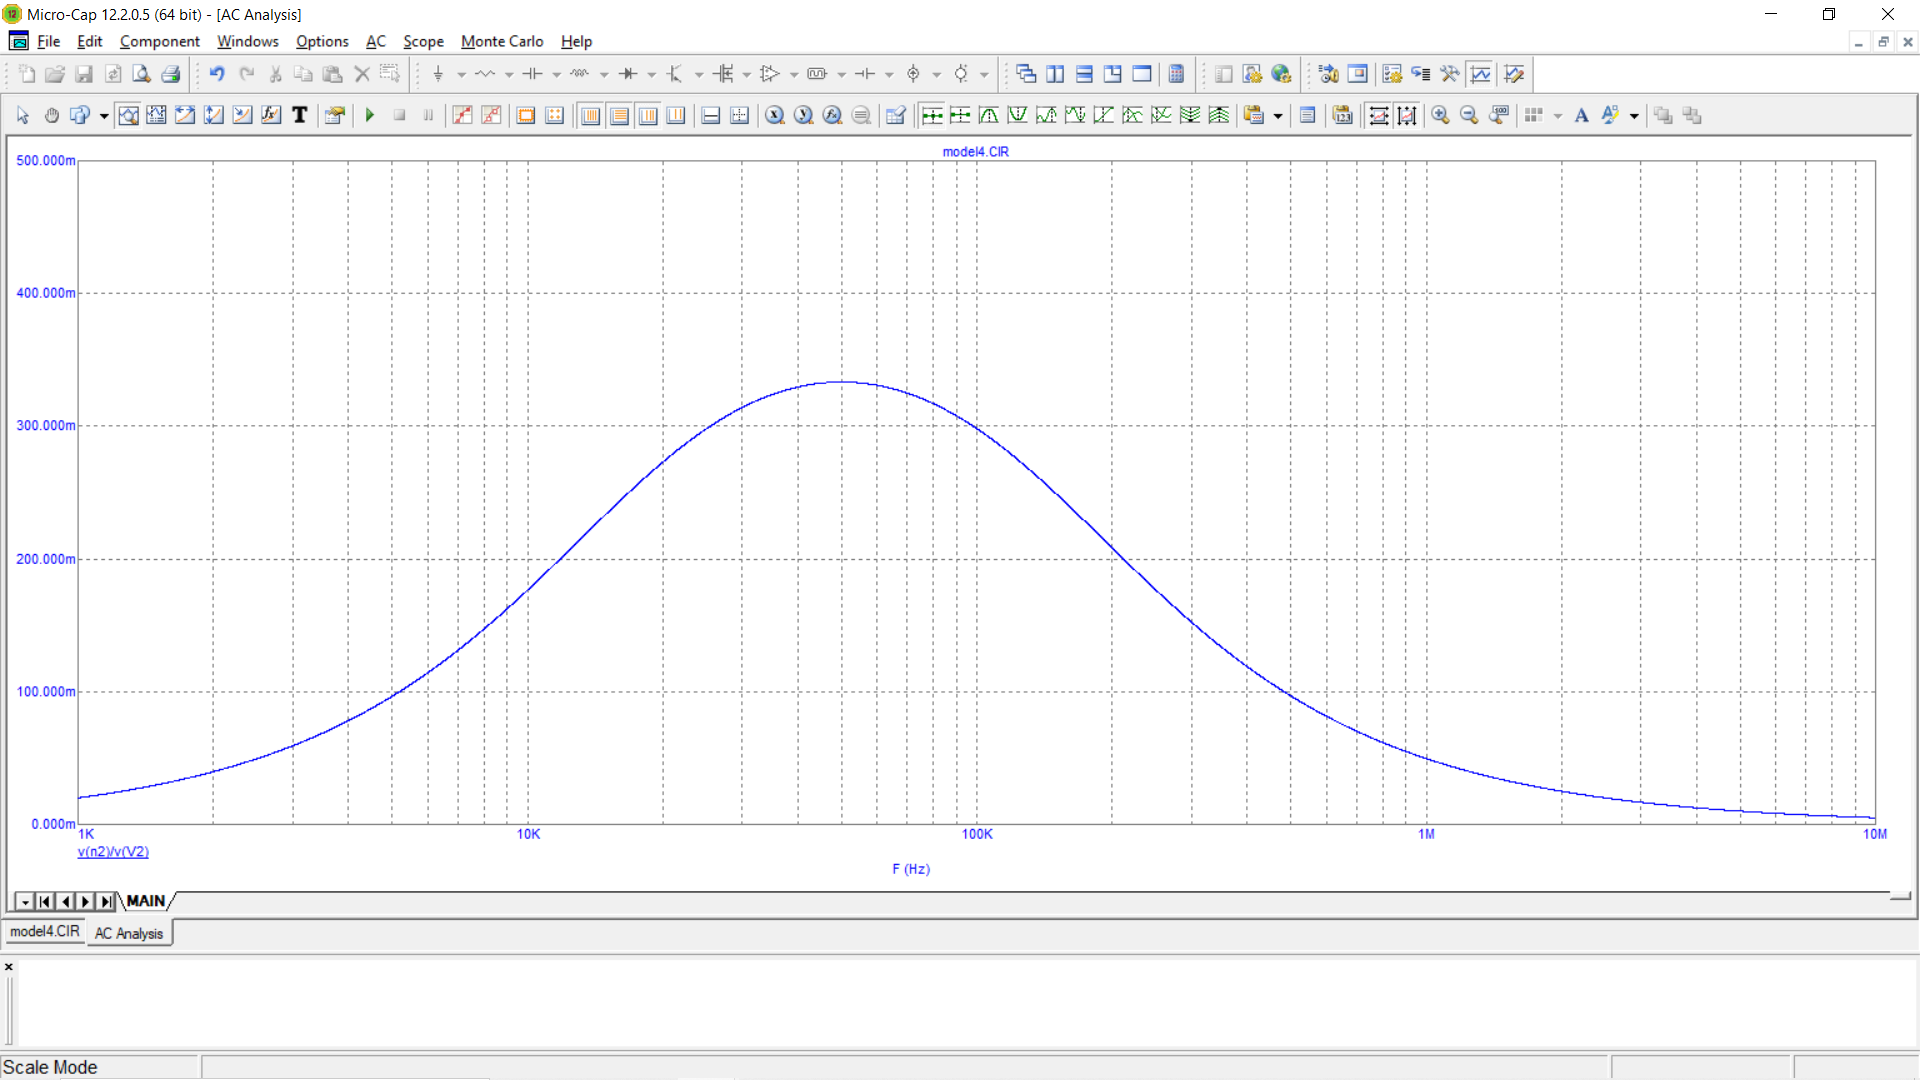
\includegraphics[scale = 0.4 \textwidth]{images/mod4_2_1.png}
    \caption{$f_0 = 50k, F = 152k, K = 0.33$, с теорией сходится}
    \label{fig:m421}
\end{figure}

\begin{figure}
    \centering
    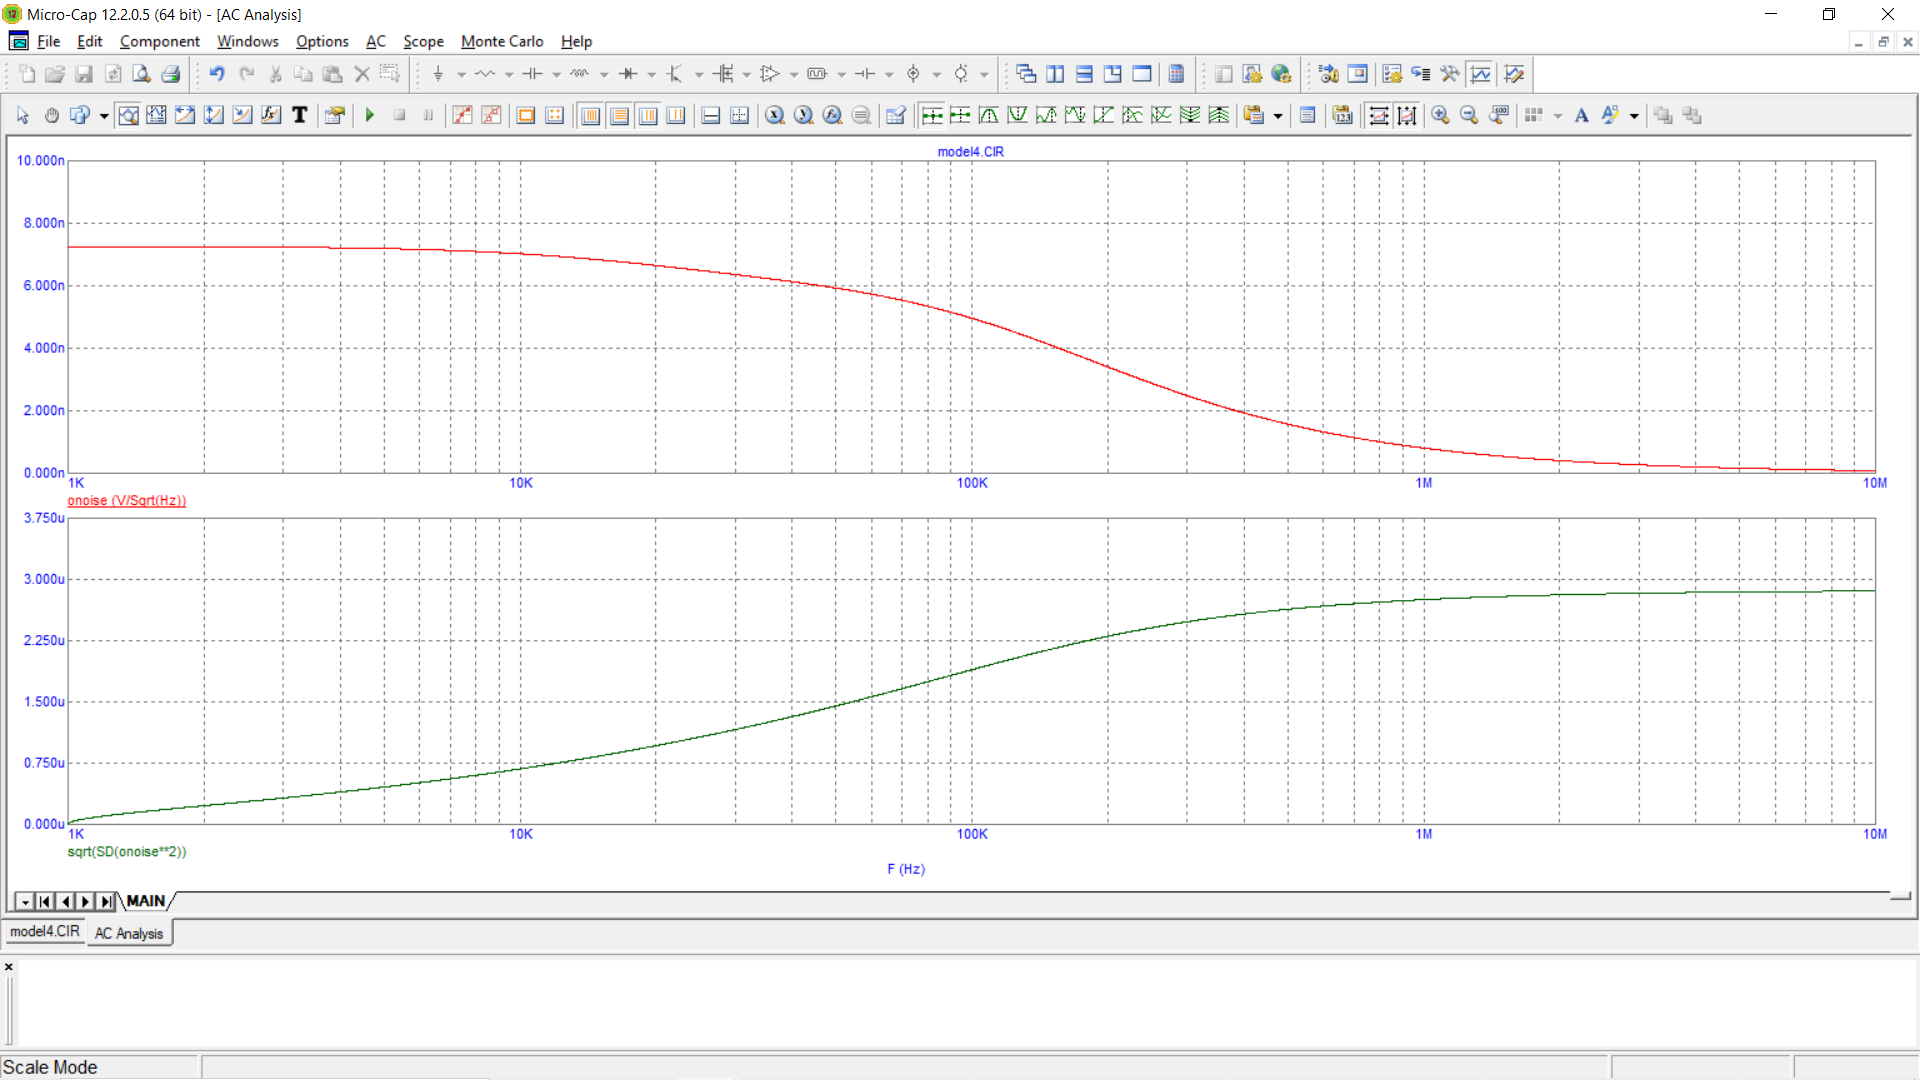
\includegraphics[scale = 0.4 \textwidth]{images/mod4_2_2_1.png}
    \caption{$n(f_0) = 5.88n, n(10 f_0) = 1.56n, \sigma = 2.86\mu$, оба резистора шумящие}
    \label{fig:m4221}
\end{figure}

\begin{figure}
    \centering
    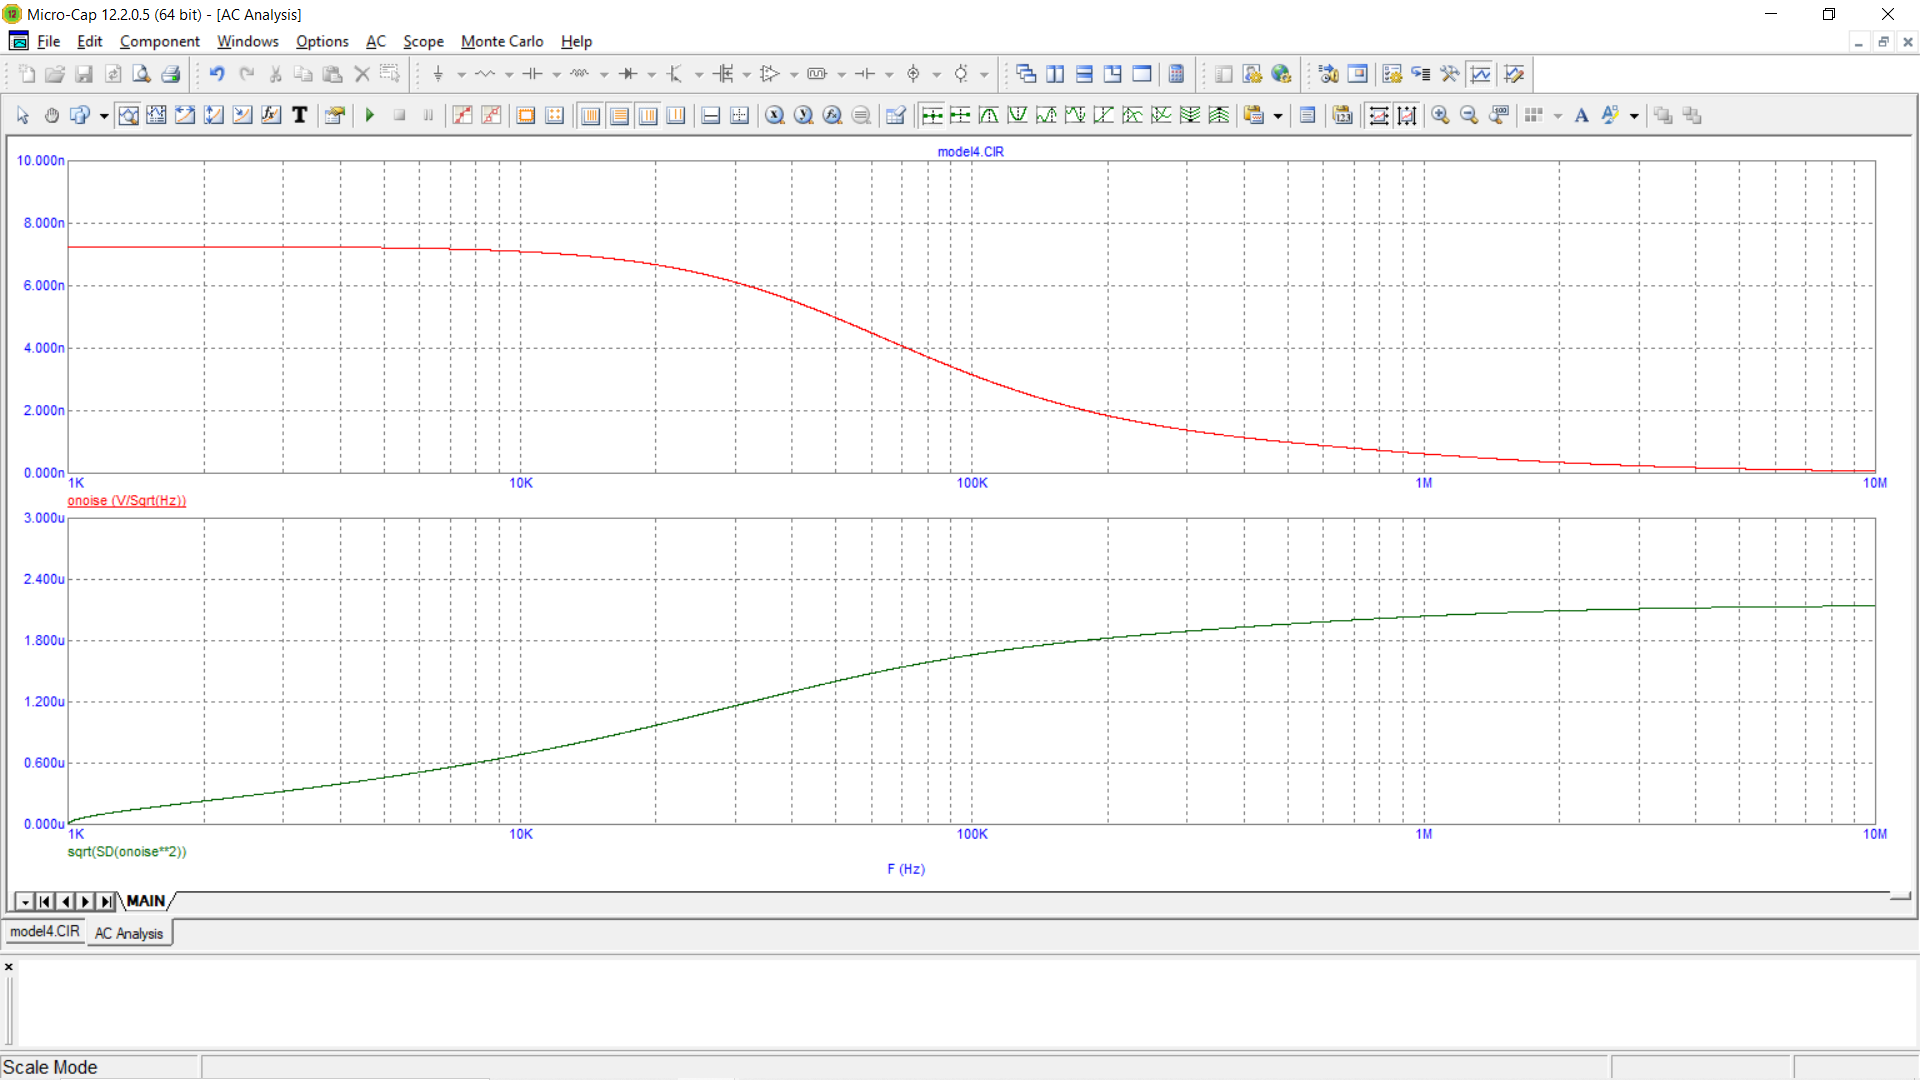
\includegraphics[scale = 0.4 \textwidth]{images/mod4_2_2_2.png}
    \caption{$n(f_0) = 4.96n, n(10 f_0) = 960p, \sigma = 2.15\mu, R_{s_2}$ не шумящий}
    \label{fig:m4222}
\end{figure}

\begin{figure}
    \centering
    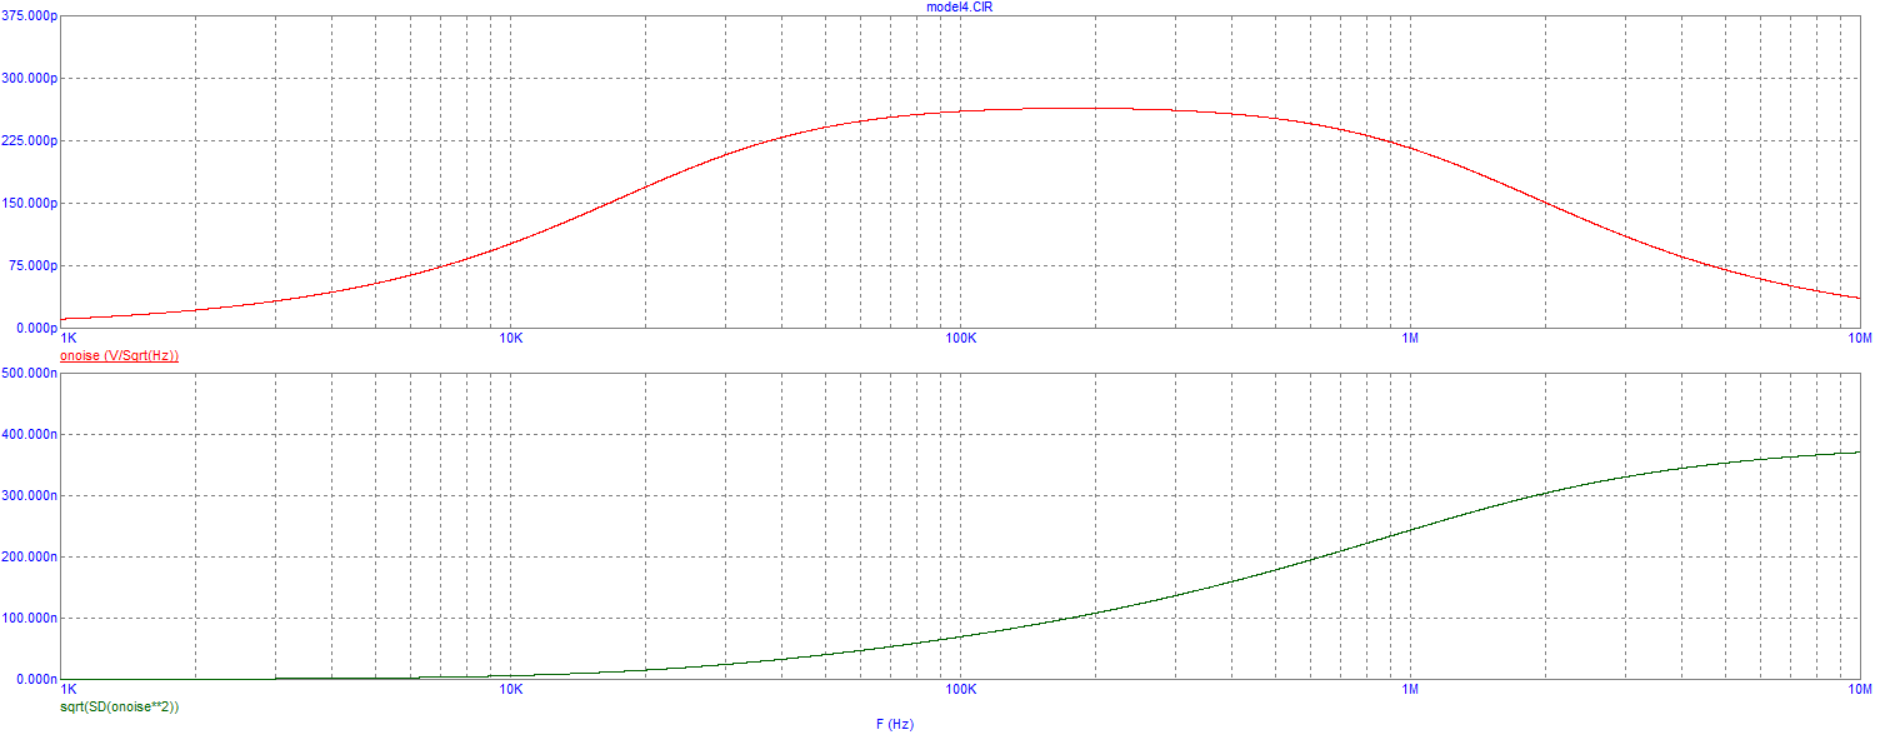
\includegraphics[scale = 0.4 \textwidth]{images/mod4_2_2_3.png}
    \caption{$n(f_0) = 240p, n(10 f_0) = 250p, \sigma = 370nб R_2$ нешумящий}
    \label{fig:m4223}
\end{figure}

\begin{figure}
    \centering
    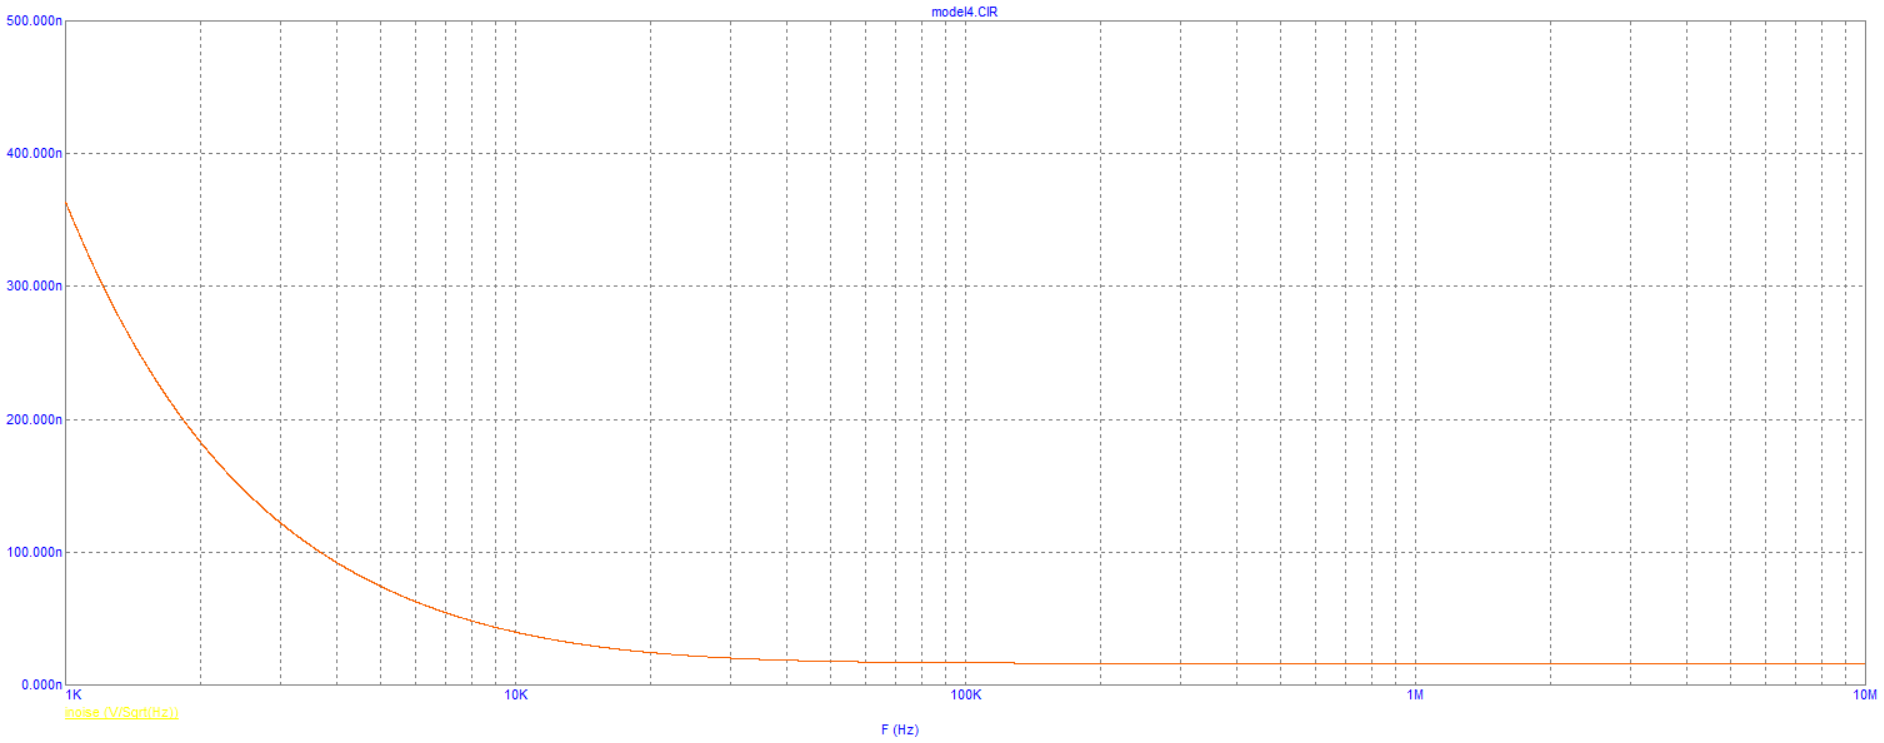
\includegraphics[scale = 0.4 \textwidth]{images/mod4_2_3.png}
    \caption{$e(f_0) = 17.7n, e(f_0/10) = 73.45n, e(f_0/100) = 728.6n => K(f_0) = 7.9, K(f_0/10) = 20.4, K(f_0/100) = 41$}
    \label{fig:m423}
\end{figure}
\FloatBarrier
\subsection{Полосовой LC-фильтр нижних частот}
\FloatBarrier
\begin{figure}[h!]
    \centering
    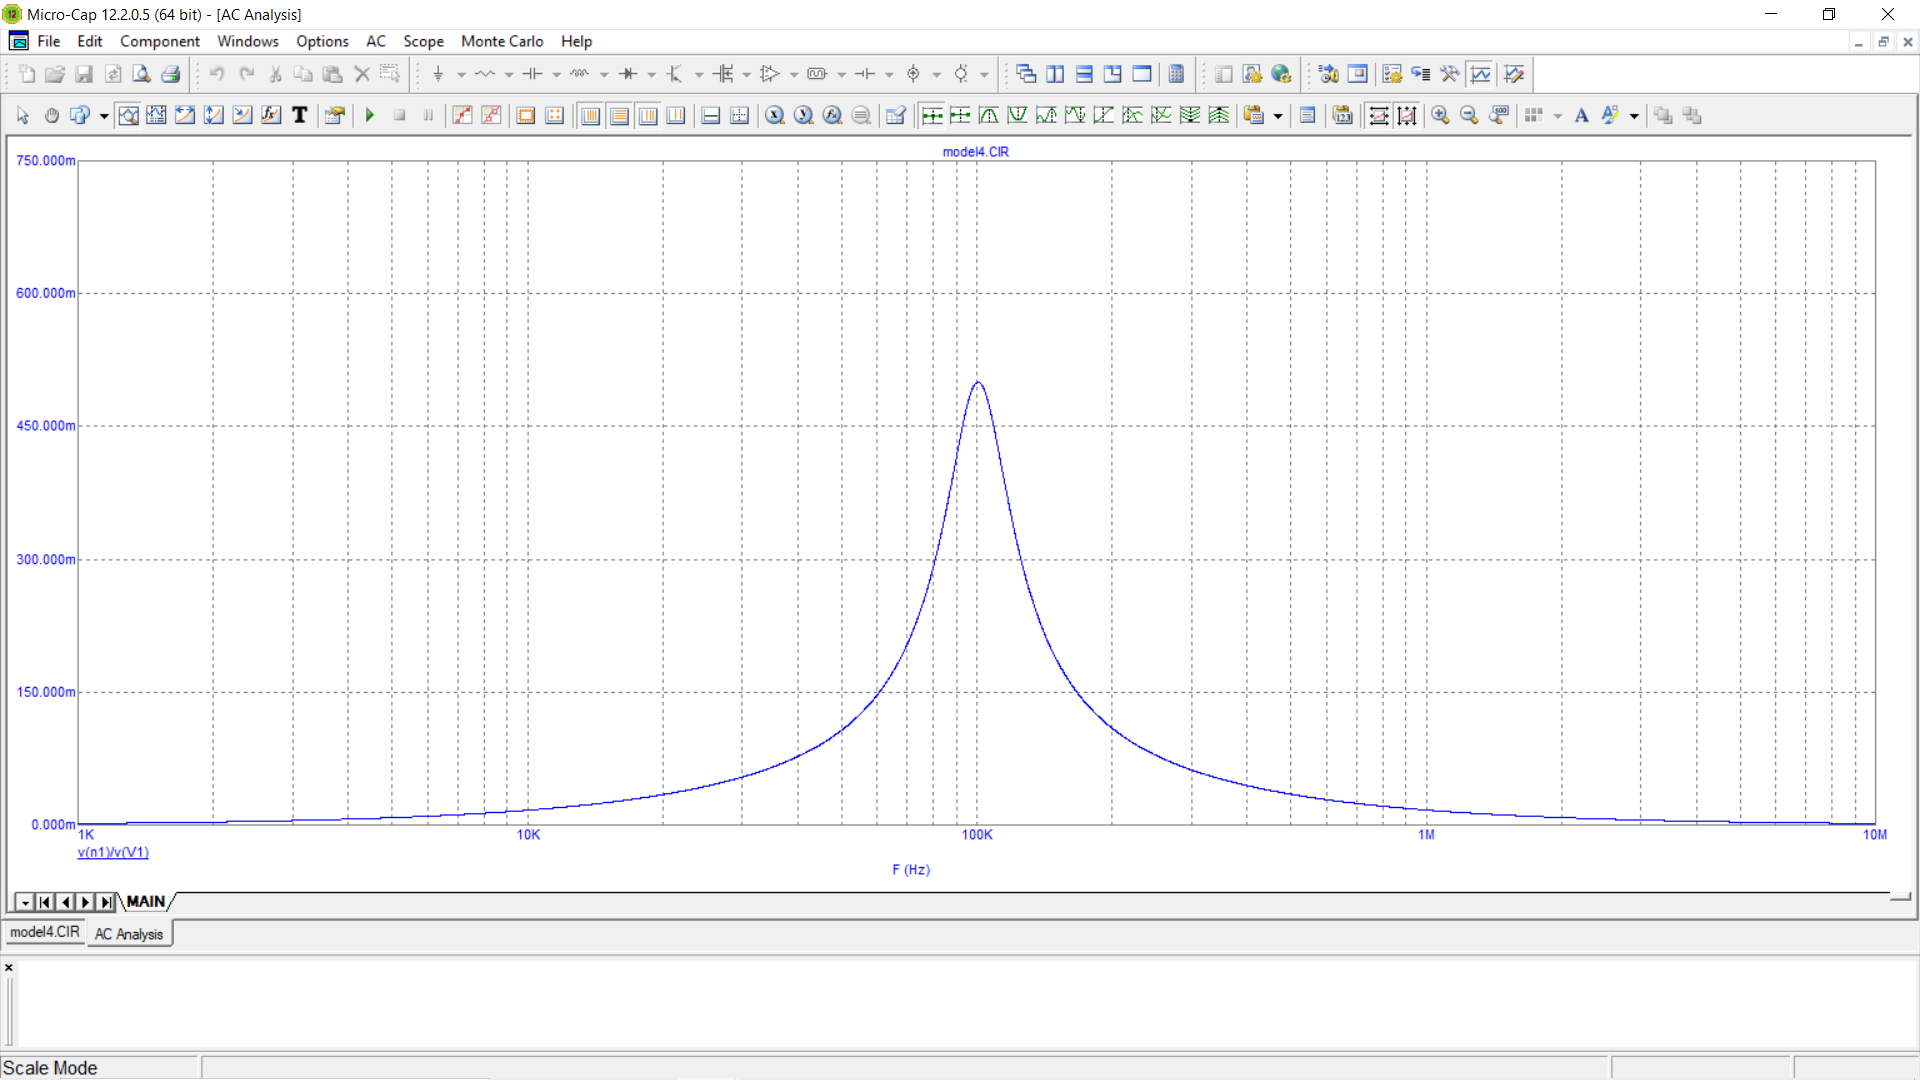
\includegraphics[scale = 0.4 \textwidth]{images/mod4_3_1.png}
    \caption{$f_0 = 102k, F = 36k, K(f_0) = 0.5, K(0) = 0.02$, с теорией сходится}
    \label{fig:m431}
\end{figure}

\begin{figure}[h!]
    \centering
    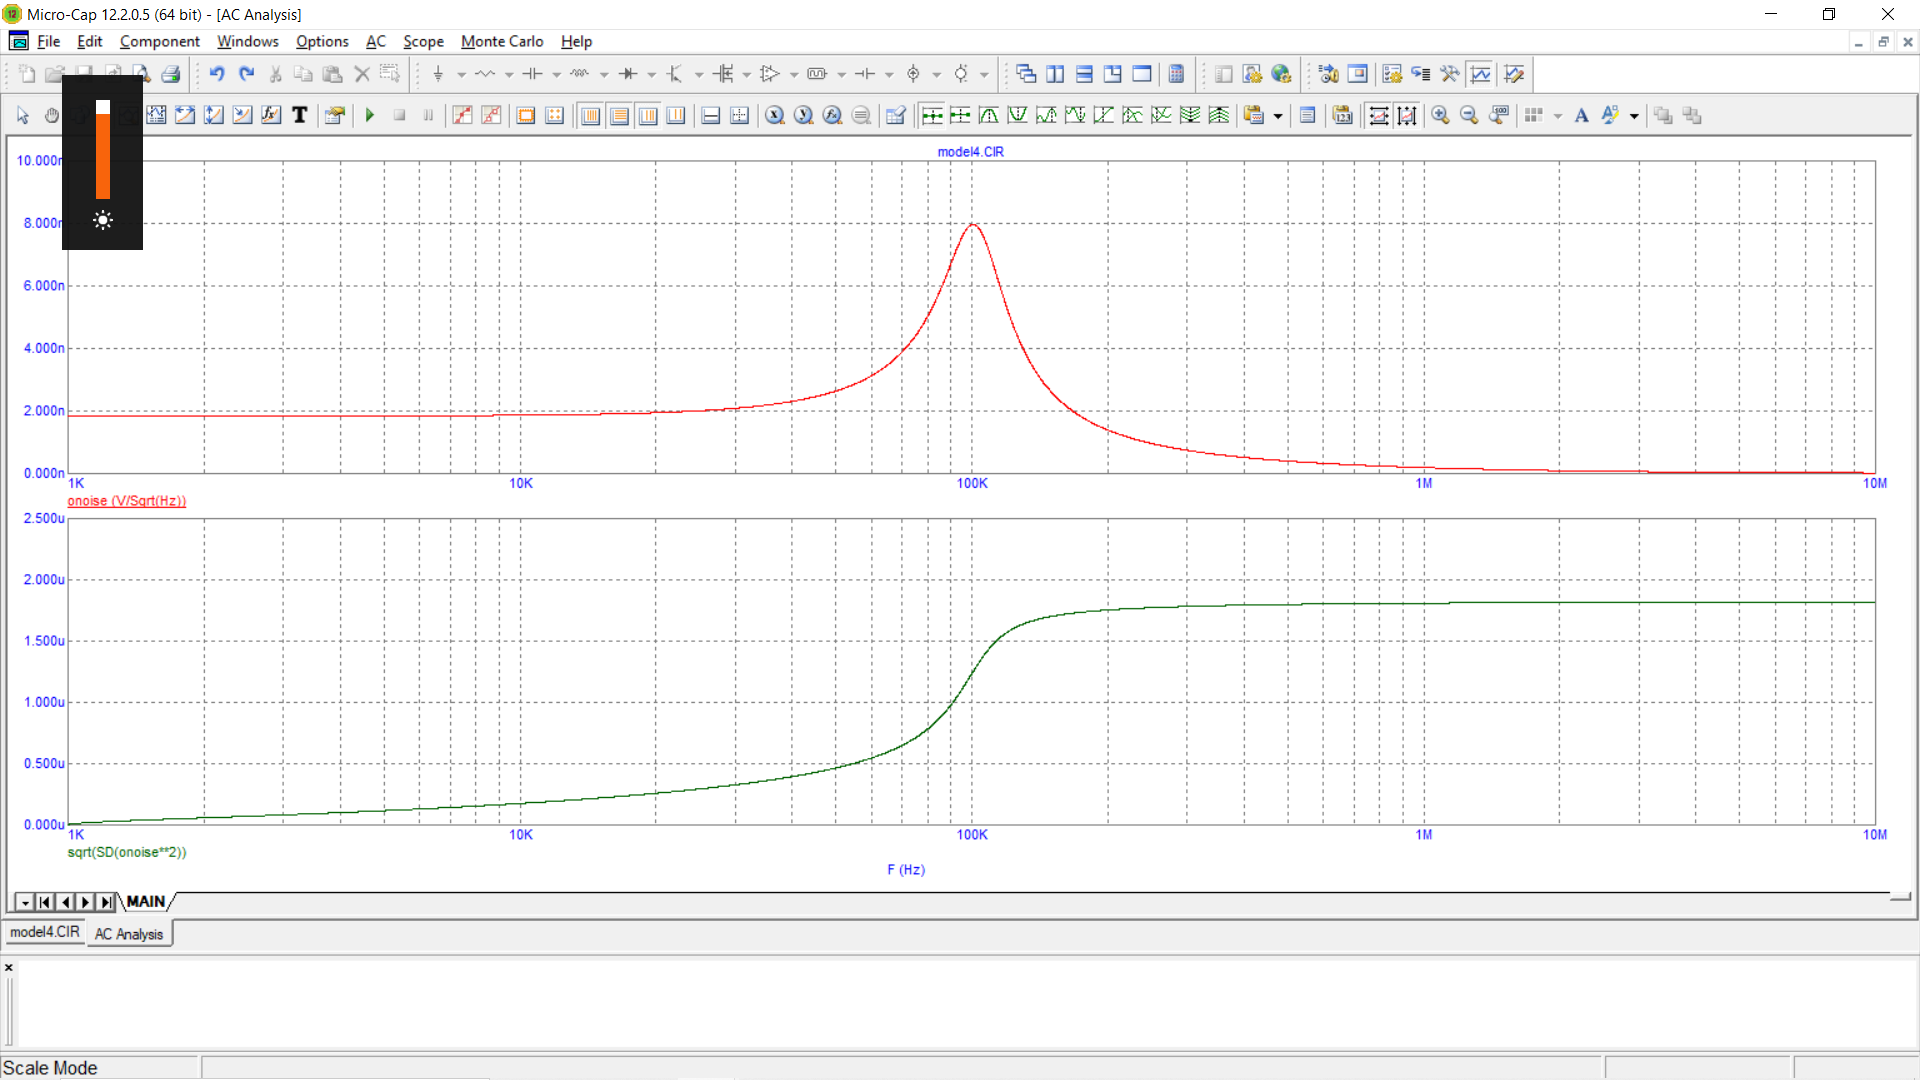
\includegraphics[scale = 0.4 \textwidth]{images/mod4_3_2_1.png}
    \caption{$n(f_0) = 7.9n, n(f_0/100) = 1.8n, \sigma = 1.8\mu$, оба шумящие}
    \label{fig:m4321}
\end{figure}

\begin{figure}[h!]
    \centering
    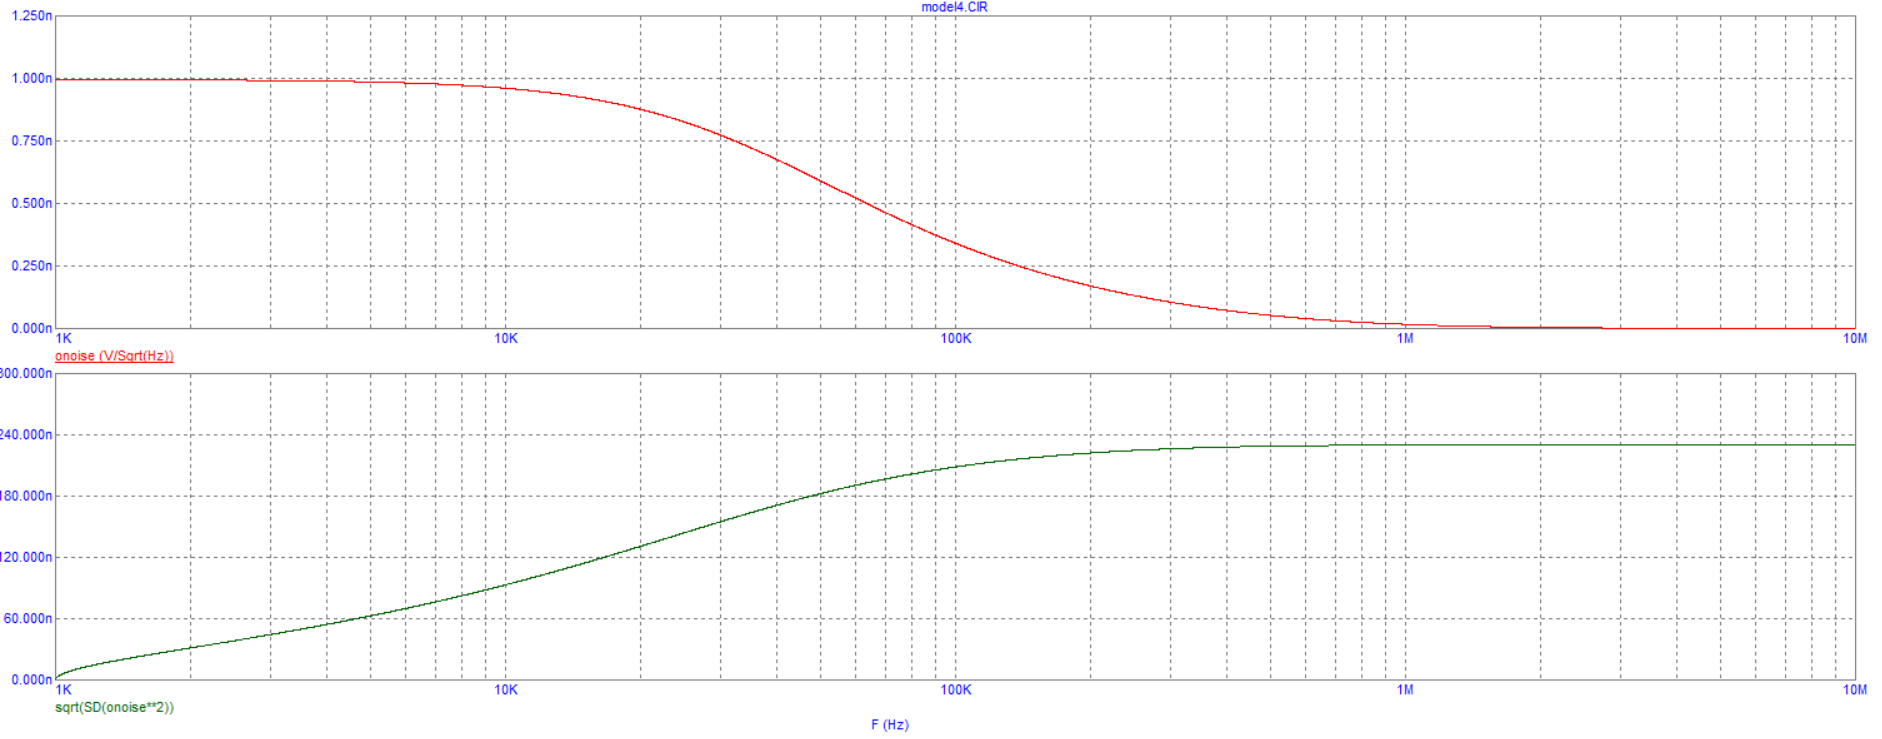
\includegraphics[scale = 0.4 \textwidth]{images/mod4_3_2_2.png}
    \caption{$n(f_0) = 355p, n(f_0/100) = 1.0n, \sigma = 228.9n, R_3$ шумящий}
    \label{fig:m4322}
\end{figure}

\begin{figure}[h!]
    \centering
    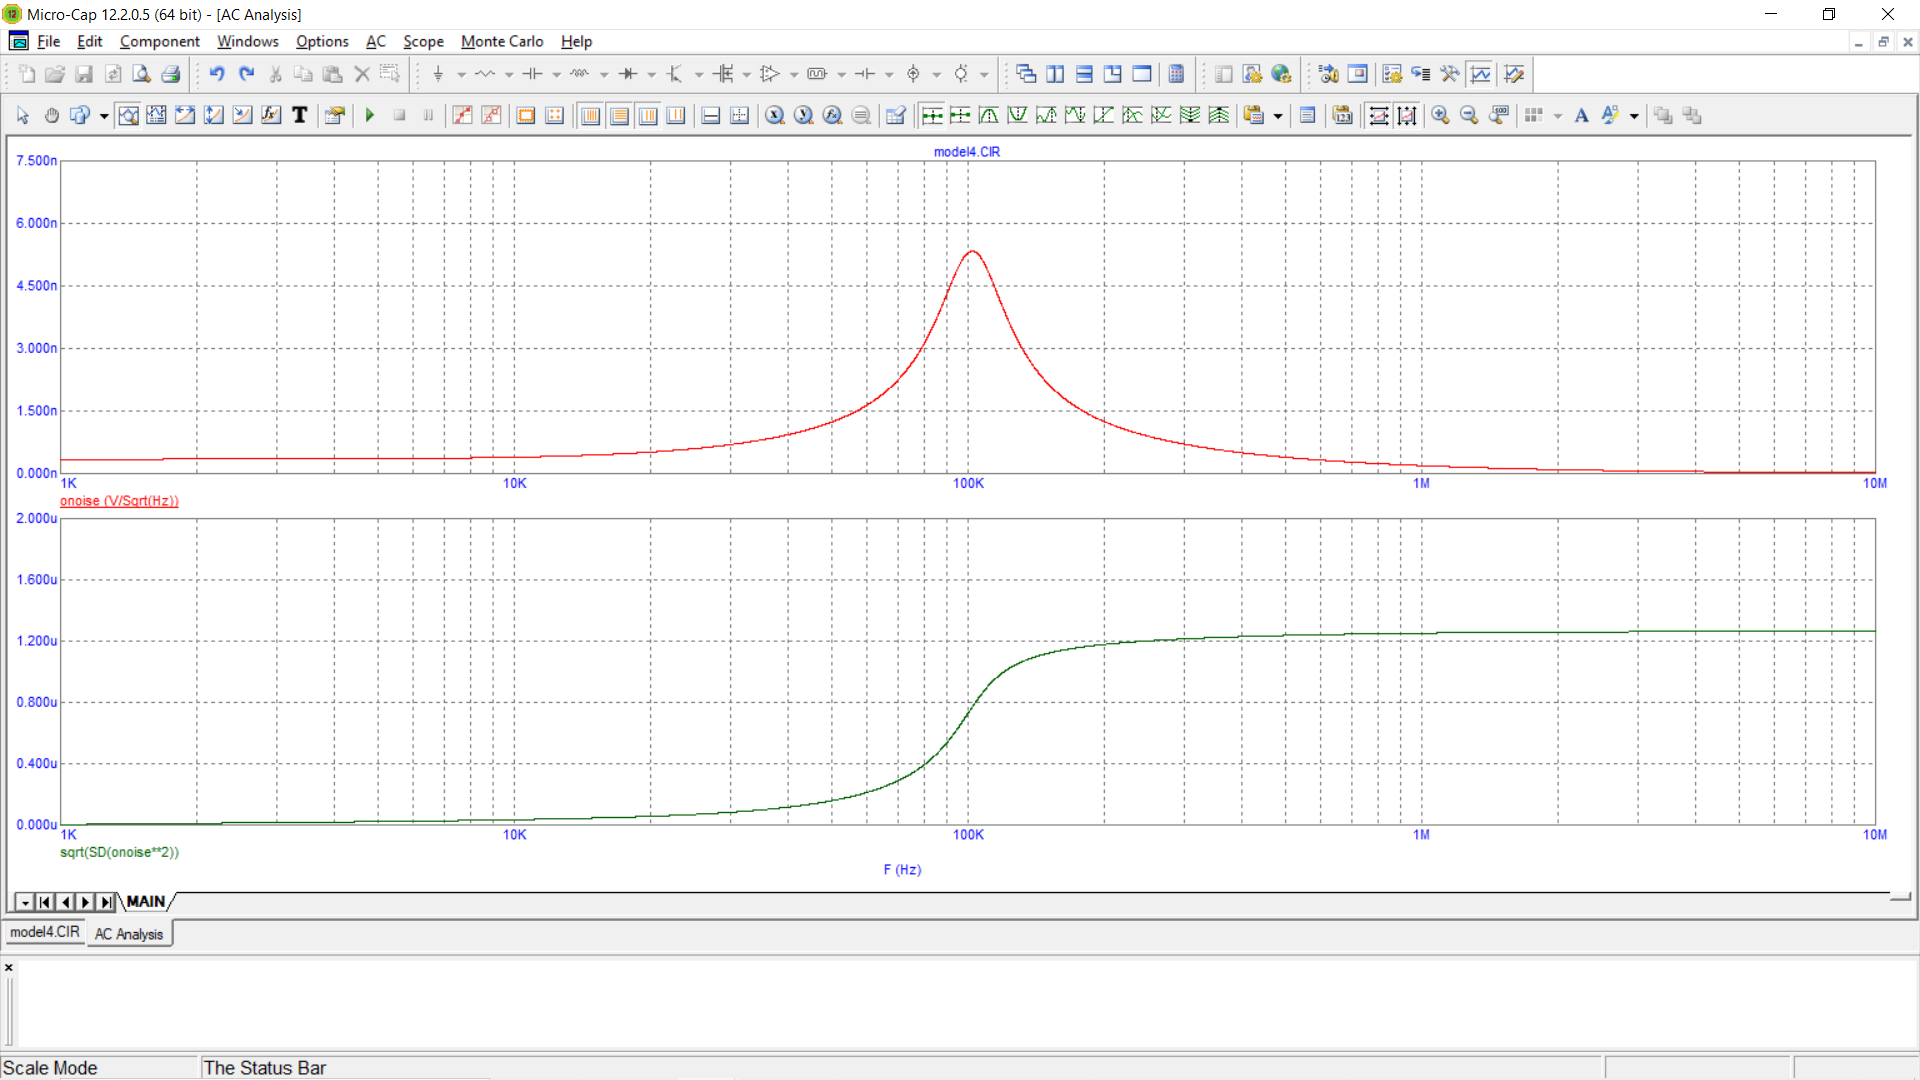
\includegraphics[scale = 0.4 \textwidth]{images/mod4_3_2_3.png}
    \caption{$n(f_0) = 1.8n, n(f_0/100) = 11.2n, \sigma = 1.7\mu, R_{s3}$ шумящий}
    \label{fig:m4322}
\end{figure}

\begin{figure}[h!]
    \centering
    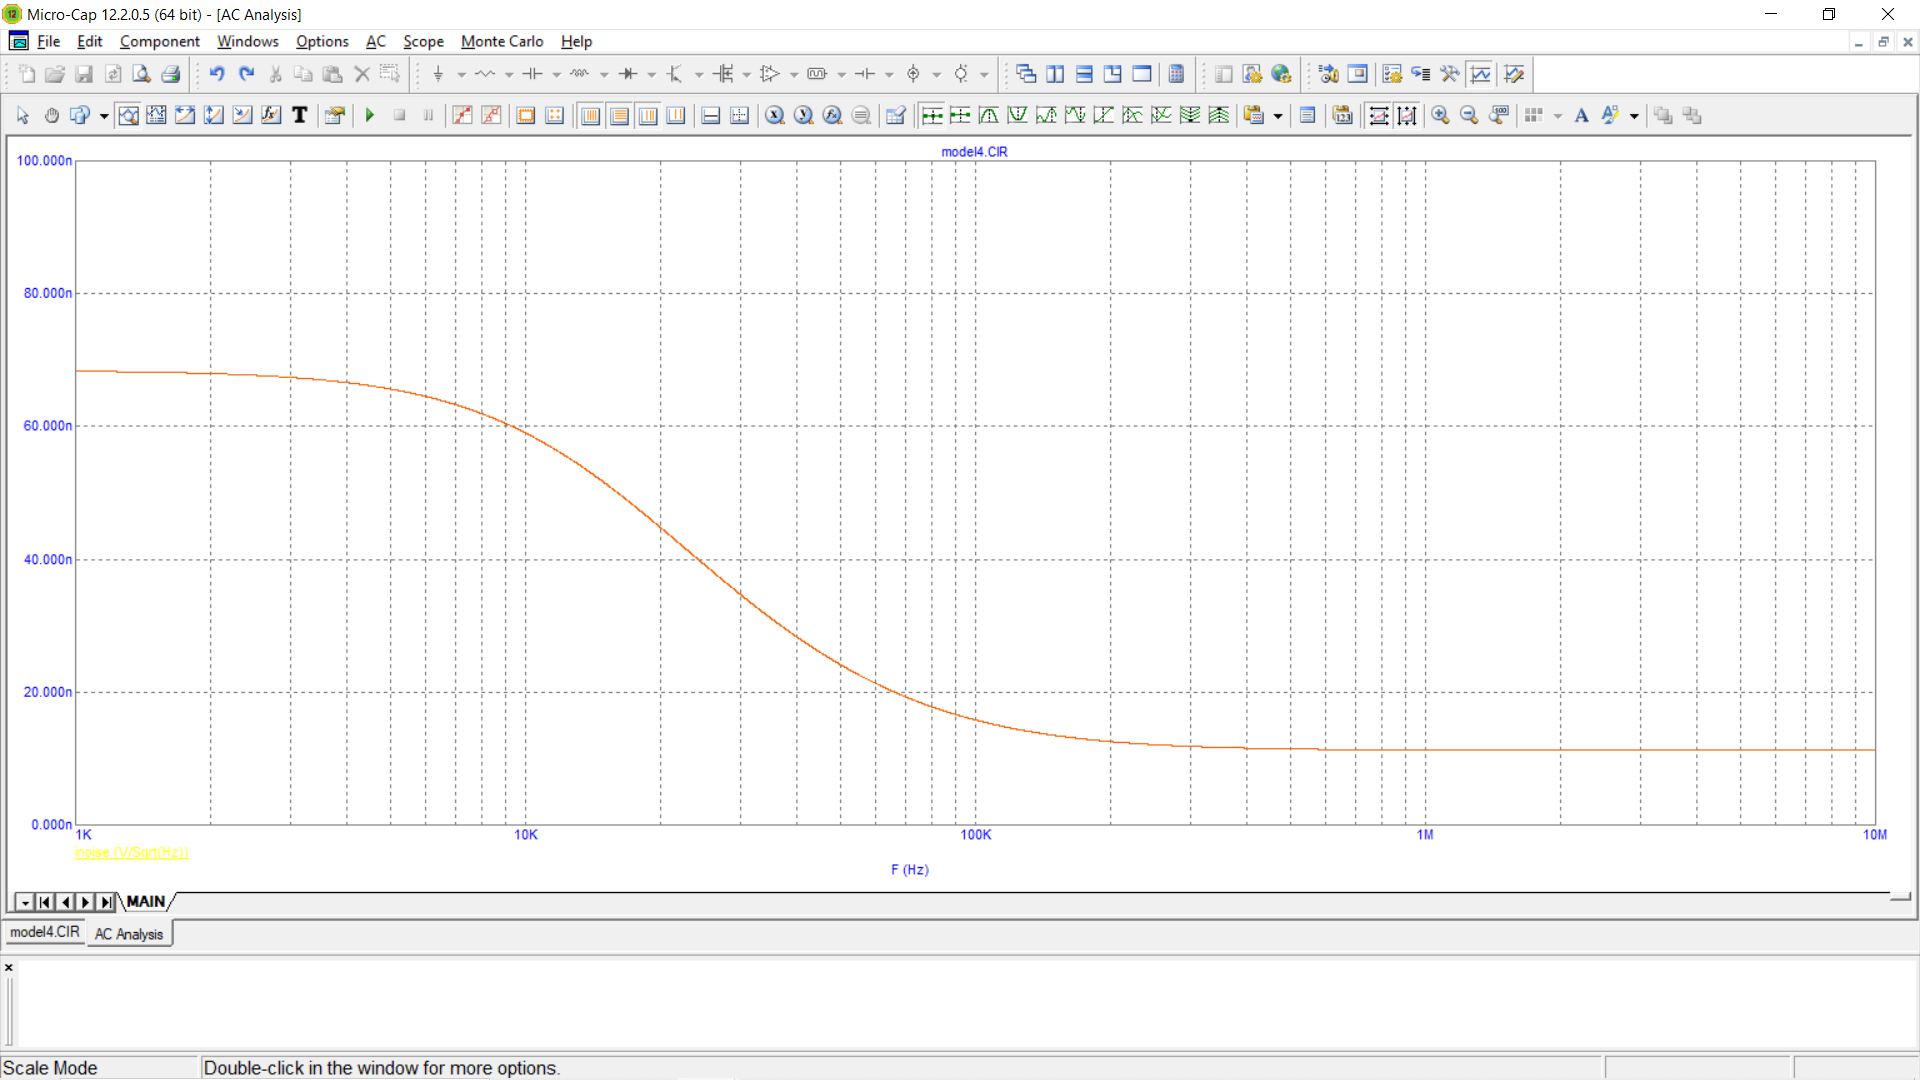
\includegraphics[scale = 0.4 \textwidth]{images/mod4_3_3.png}
    \caption{$e(f_0) = 15.4n, e(f_0/100) = 68.3n, e(10 f_0) = 10.9n => K(f_0) = 31.5, K(f_0/100) = 18.9, K(10 f_0) = 15.8$}
    \label{fig:m433}
\end{figure}
\FloatBarrier
\section{\textbf{model5}}
\FloatBarrier
$I_c = 125\mu, r_b = 112.5$ Ом

\subsection{Измерение шумового коллекторного тока}
\FloatBarrier
\subsubsection{}
\FloatBarrier
\begin{figure}
    \centering
    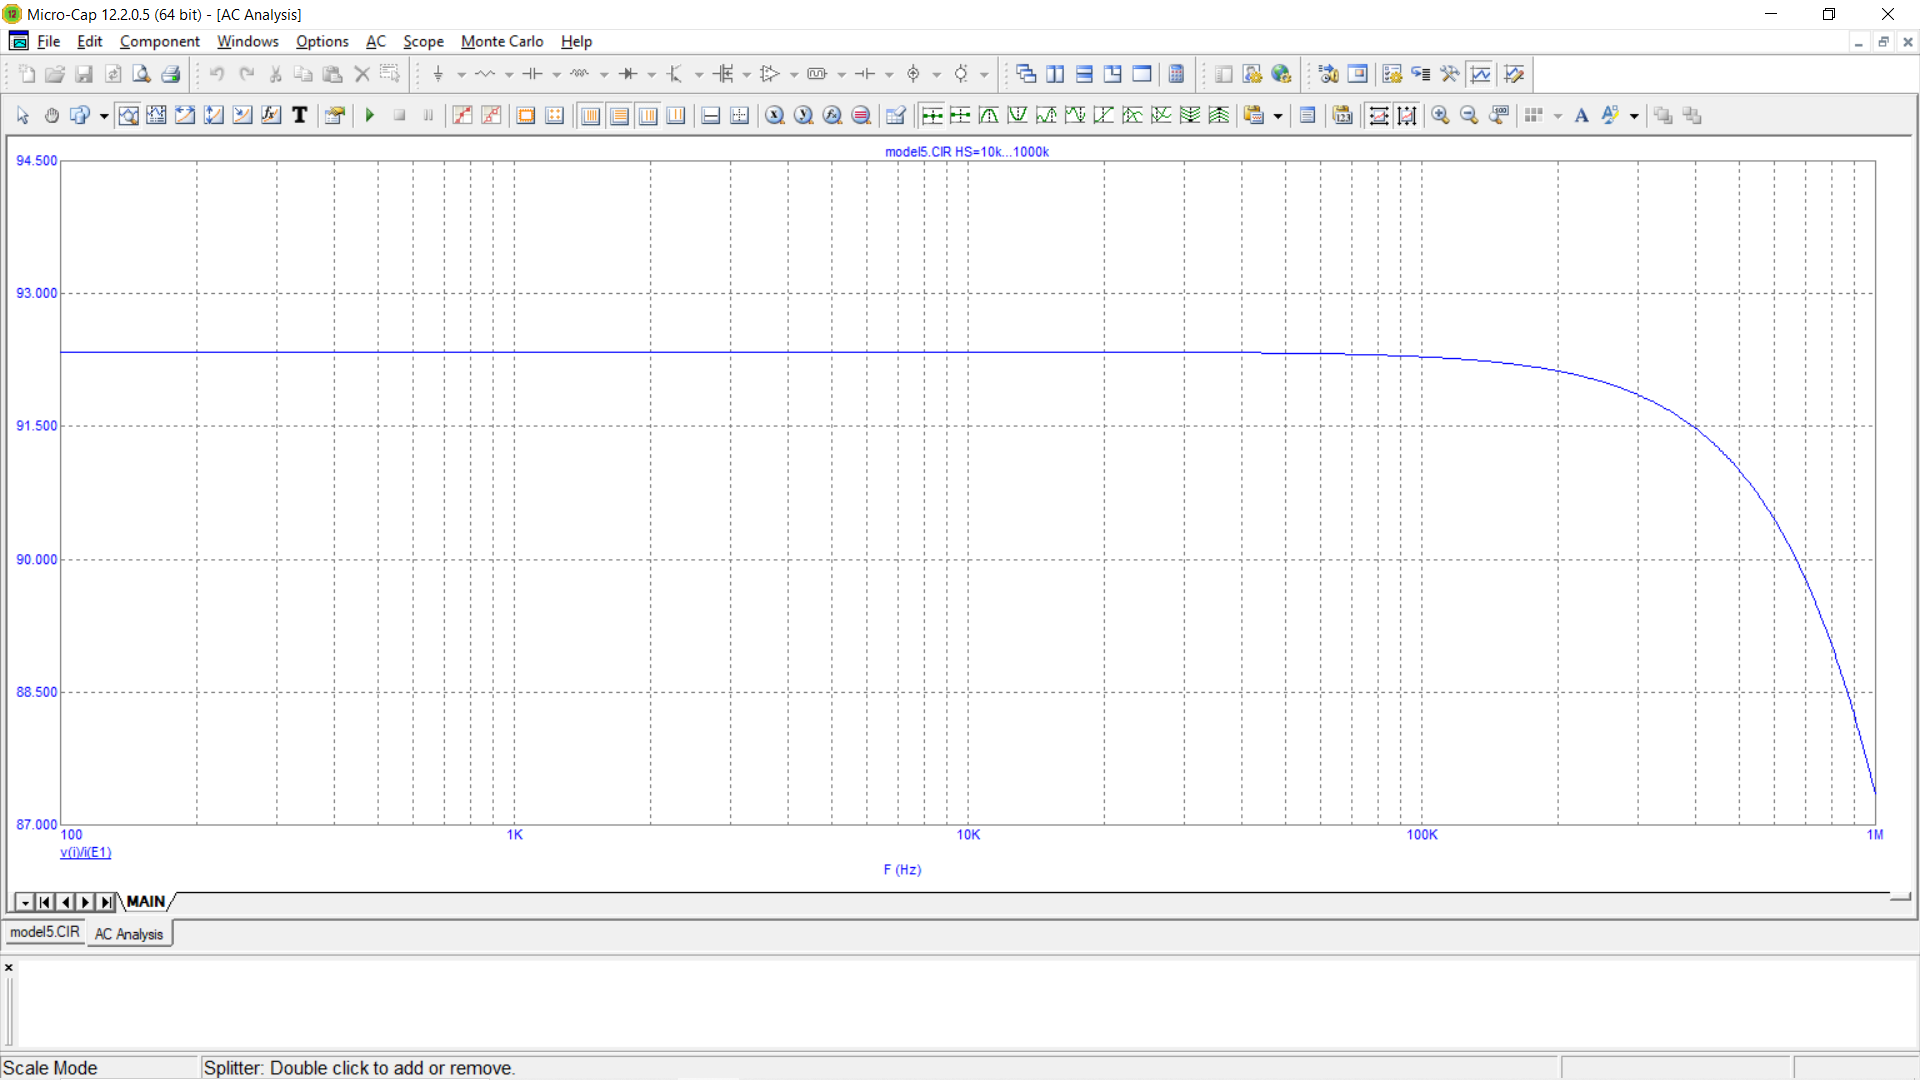
\includegraphics[scale = 0.4 \textwidth]{images/mod5_1_1.png}
    \caption{$h_{21}$ = 84.9}
    \label{fig:m511}
\end{figure}
\FloatBarrier
\subsubsection{}
\FloatBarrier
\begin{figure}[h!]
    \centering
    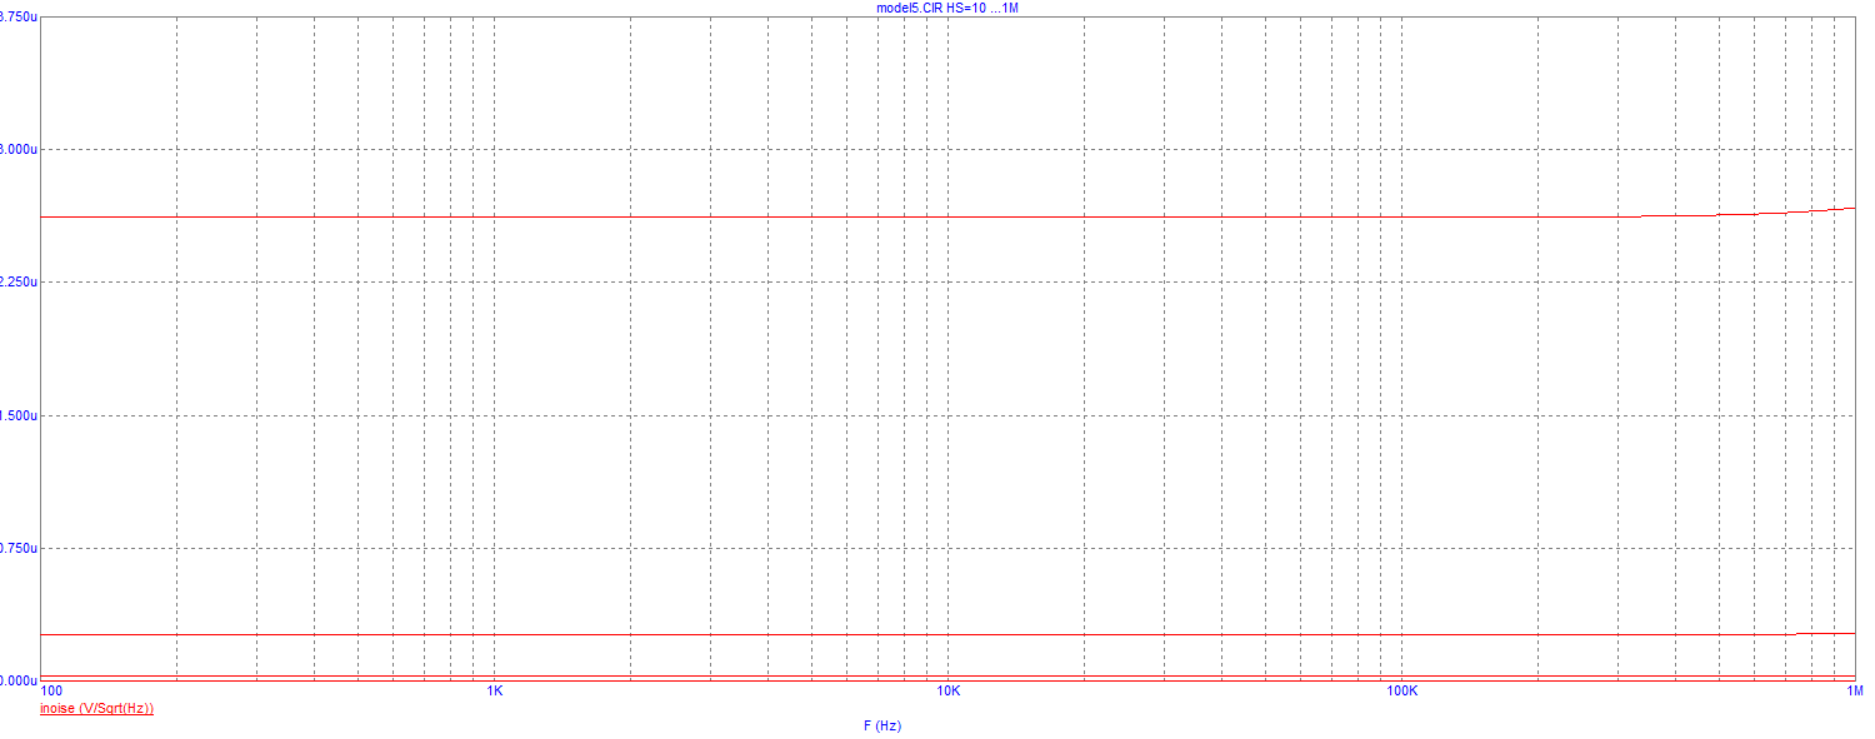
\includegraphics[scale = 0.4 \textwidth]{images/mod5_1_2_1.png}
    \caption{Варьирование $H_s = [10, 1000k|Log10]$}
    \label{fig:m5121}
\end{figure}

\begin{figure}[h!]
    \centering
    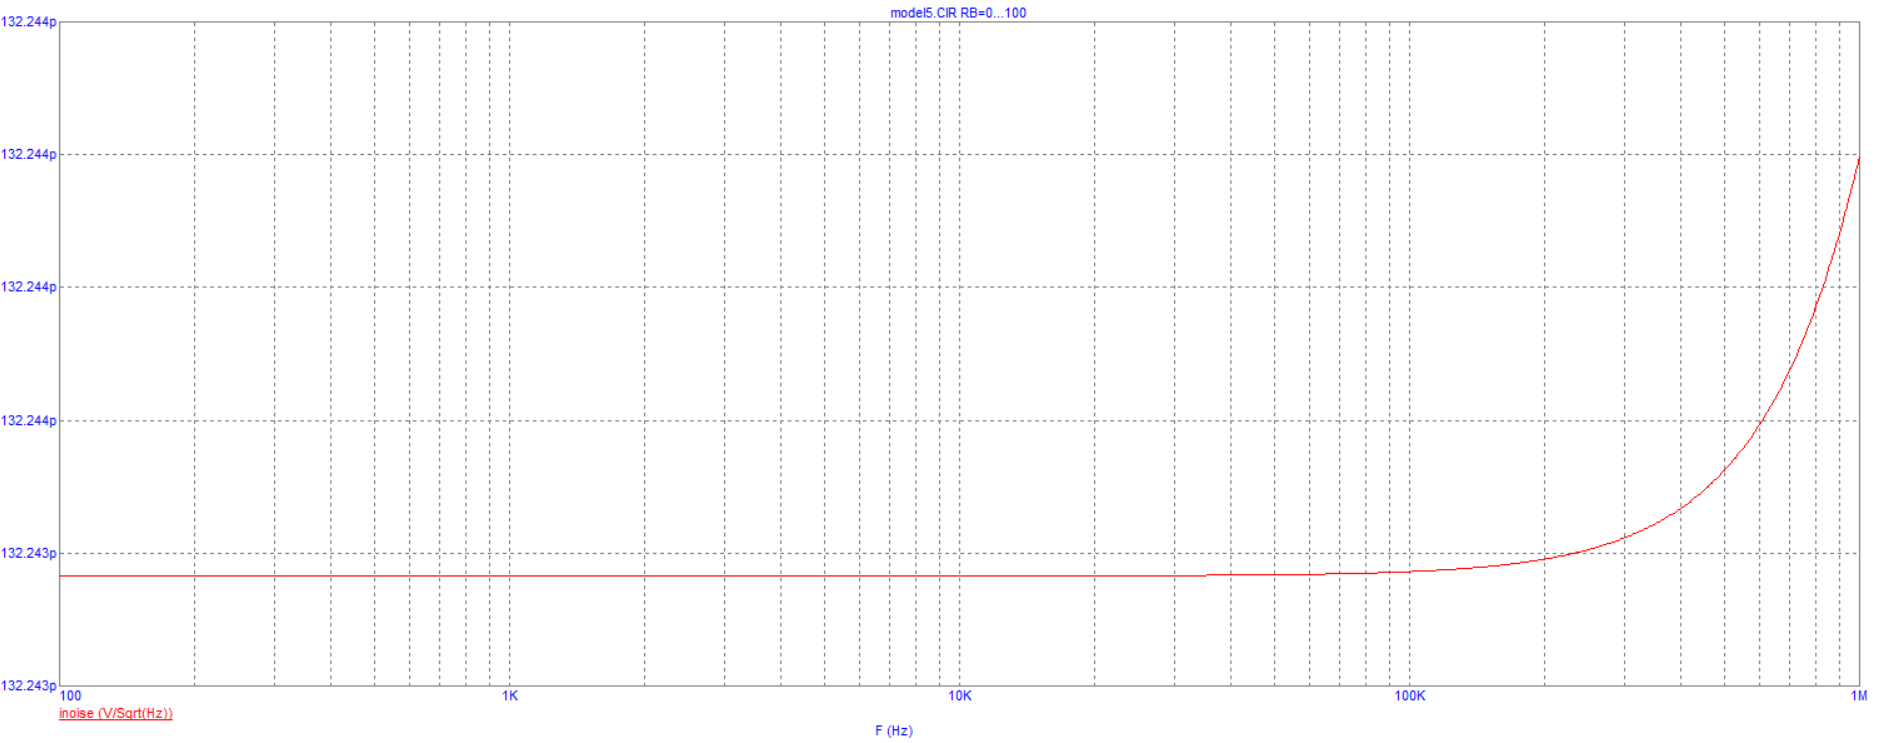
\includegraphics[scale = 0.4 \textwidth]{images/mod5_1_2_2.png}
    \caption{Варьирование $RB = [0, 100|25]$}
    \label{fig:m5122}
\end{figure}
\FloatBarrier
\subsubsection{}
\FloatBarrier
\begin{figure}
    \centering
    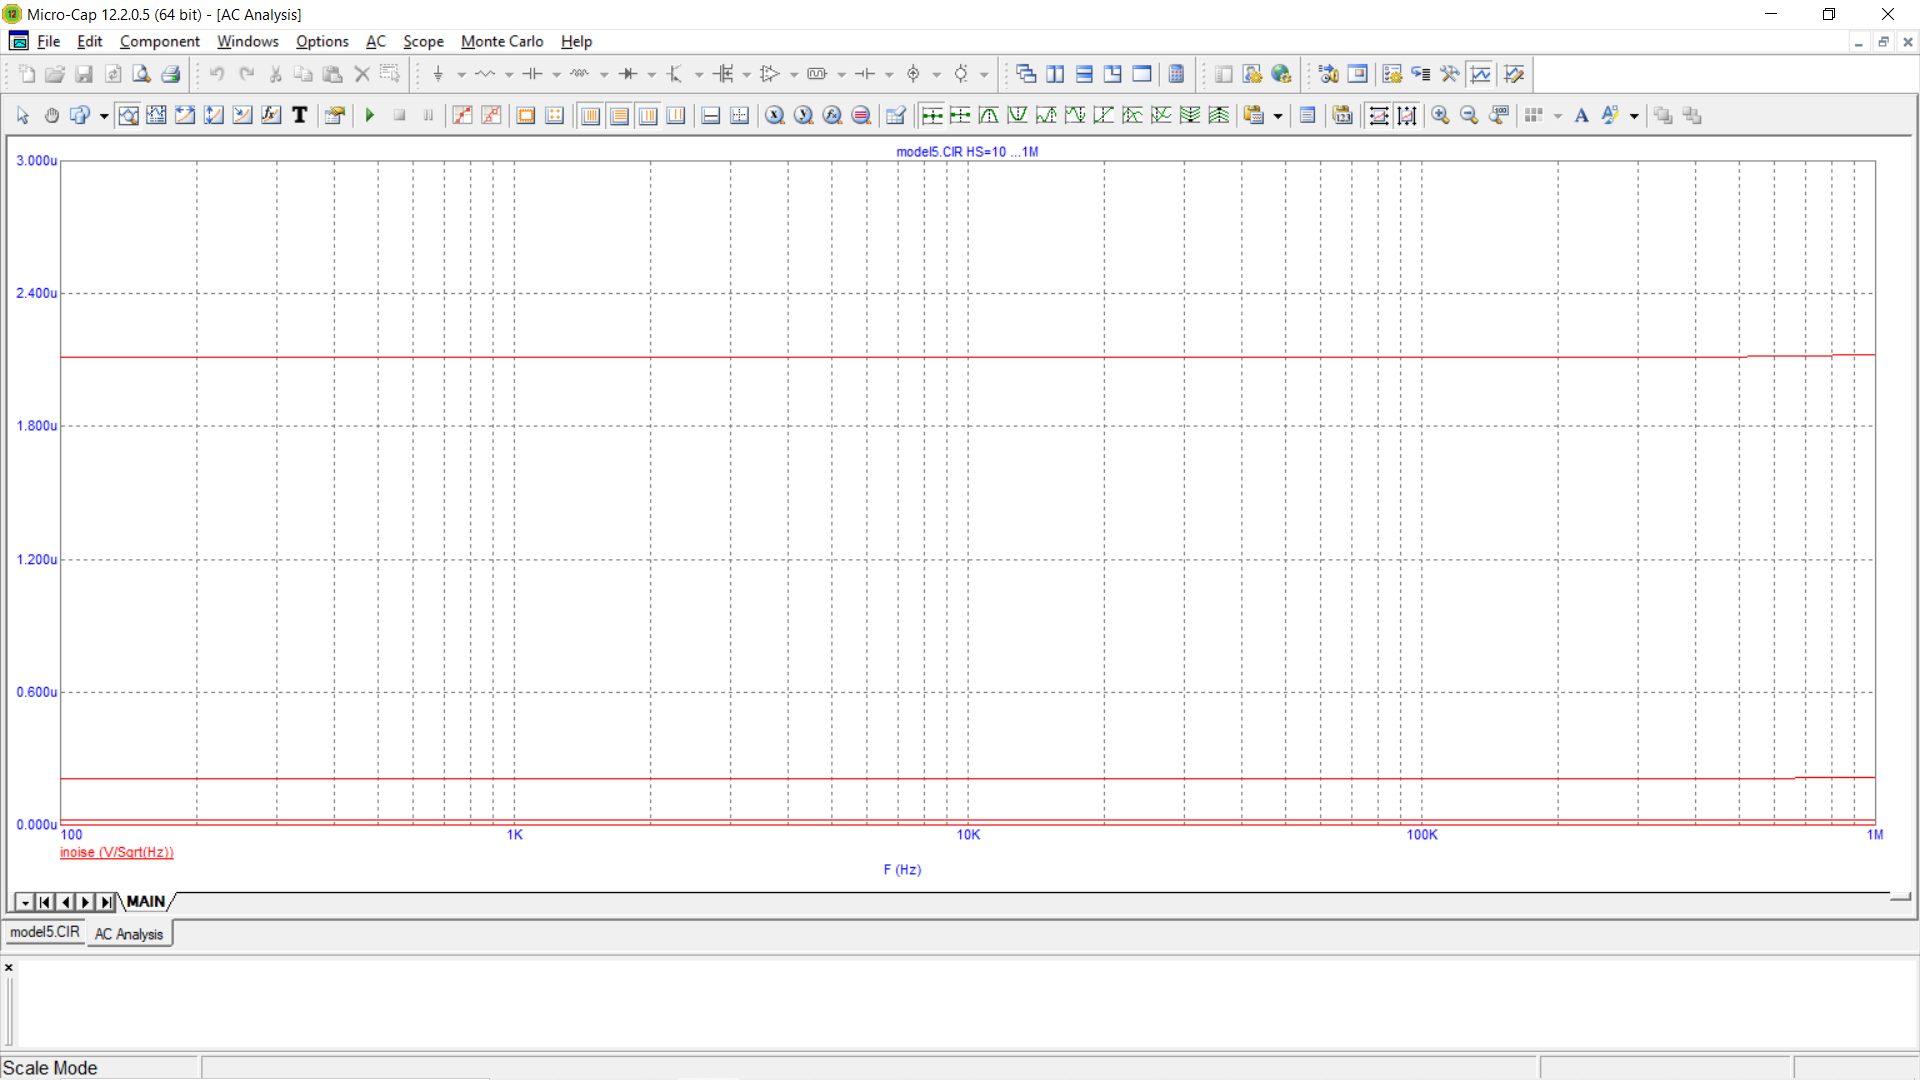
\includegraphics[scale = 0.4 \textwidth]{images/mod5_1_3_1.png}
    \caption{Варьирование $H_s = [10, 1000|Log10]$ для $I_c = 0.1m, I_1 = 1.83\mu$}
    \label{fig:m5131}
\end{figure}

\begin{figure}[h!]
    \centering
    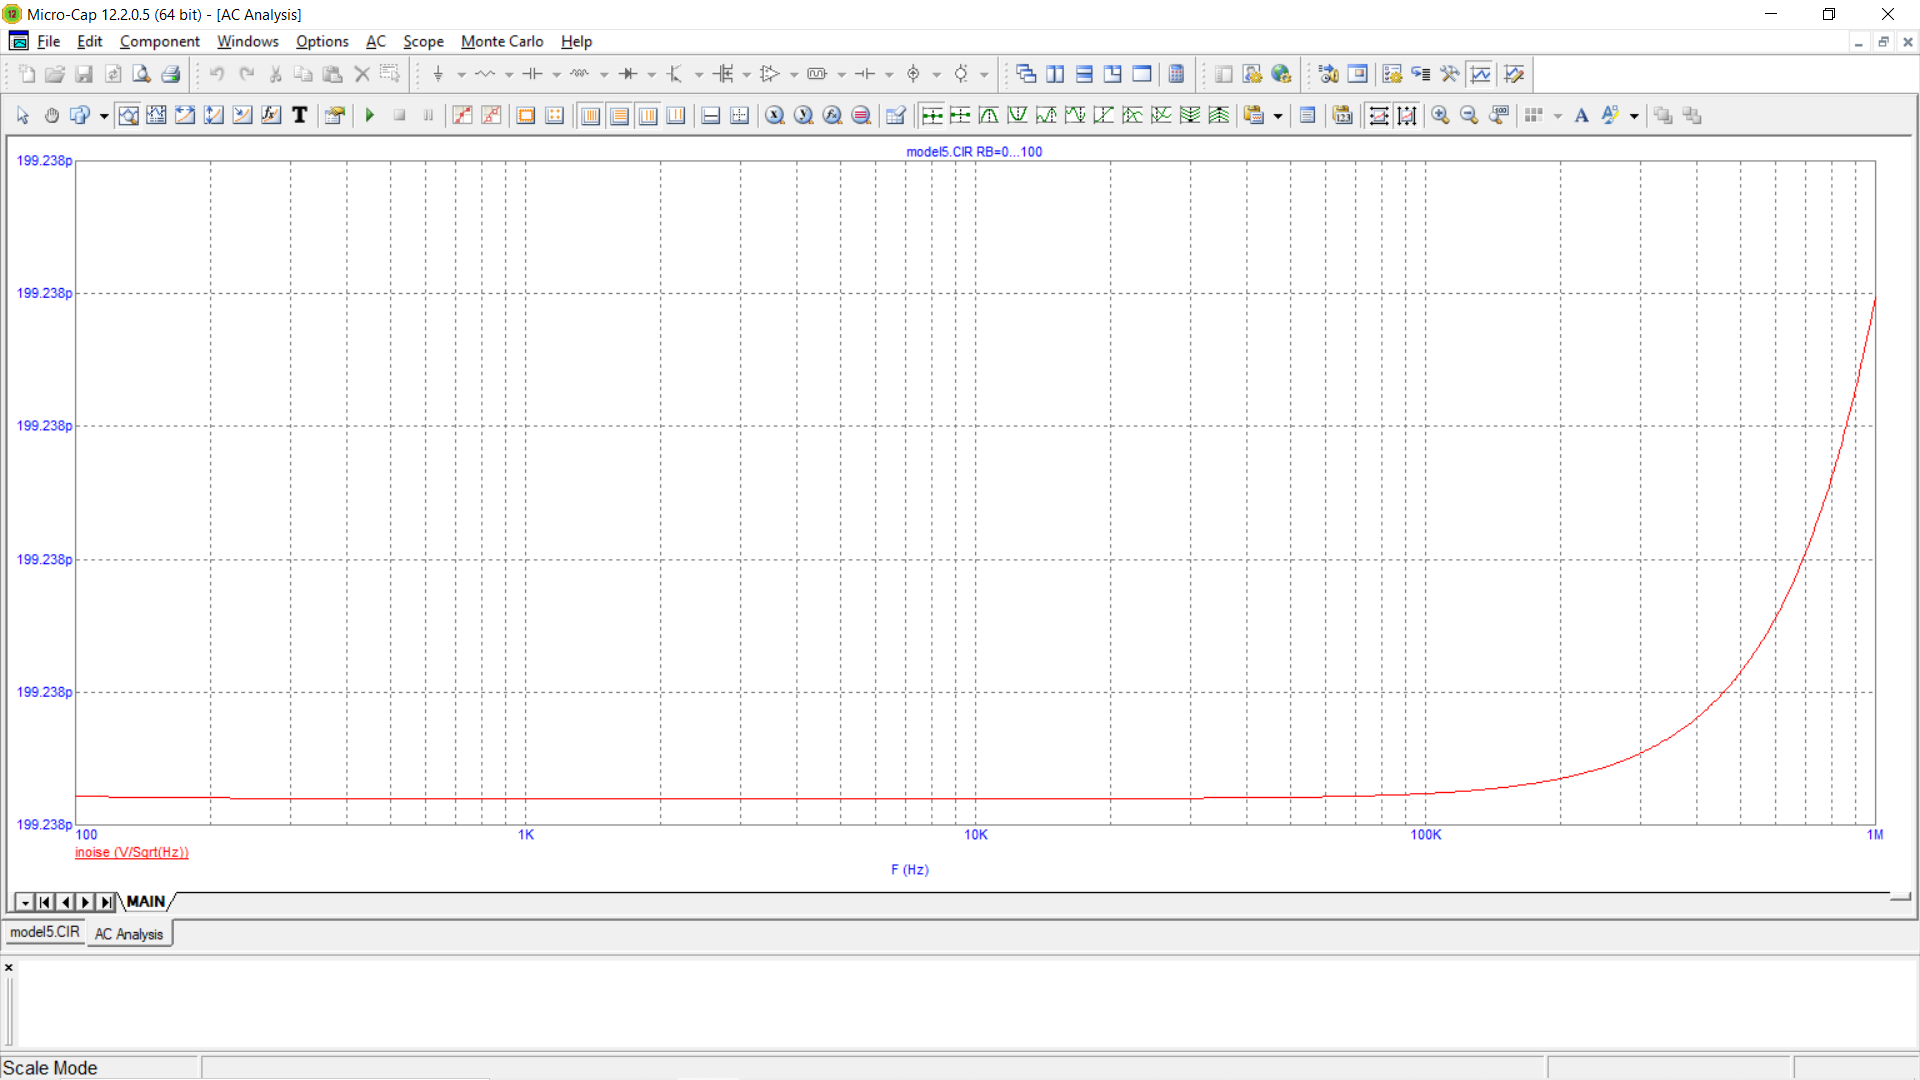
\includegraphics[scale = 0.4 \textwidth]{images/mod5_1_3_2.png}
    \caption{Варьирование $RB = [0, 100|25]$ для $I_c = 0.1m, I_1 = 1.83\mu$}
    \label{fig:m5132}
\end{figure}
\FloatBarrier
\subsection{Измерение коэффициента шума}
\FloatBarrier
$R_s$ = 40k.

\section{\textbf{model6}}

$U_p = 1.1$ В, $R_g = 25$ Ом, $I_d = 1m?$
\FloatBarrier
\subsection{Исследование шумового тока}
\FloatBarrier
\begin{figure}[h!]
    \centering
    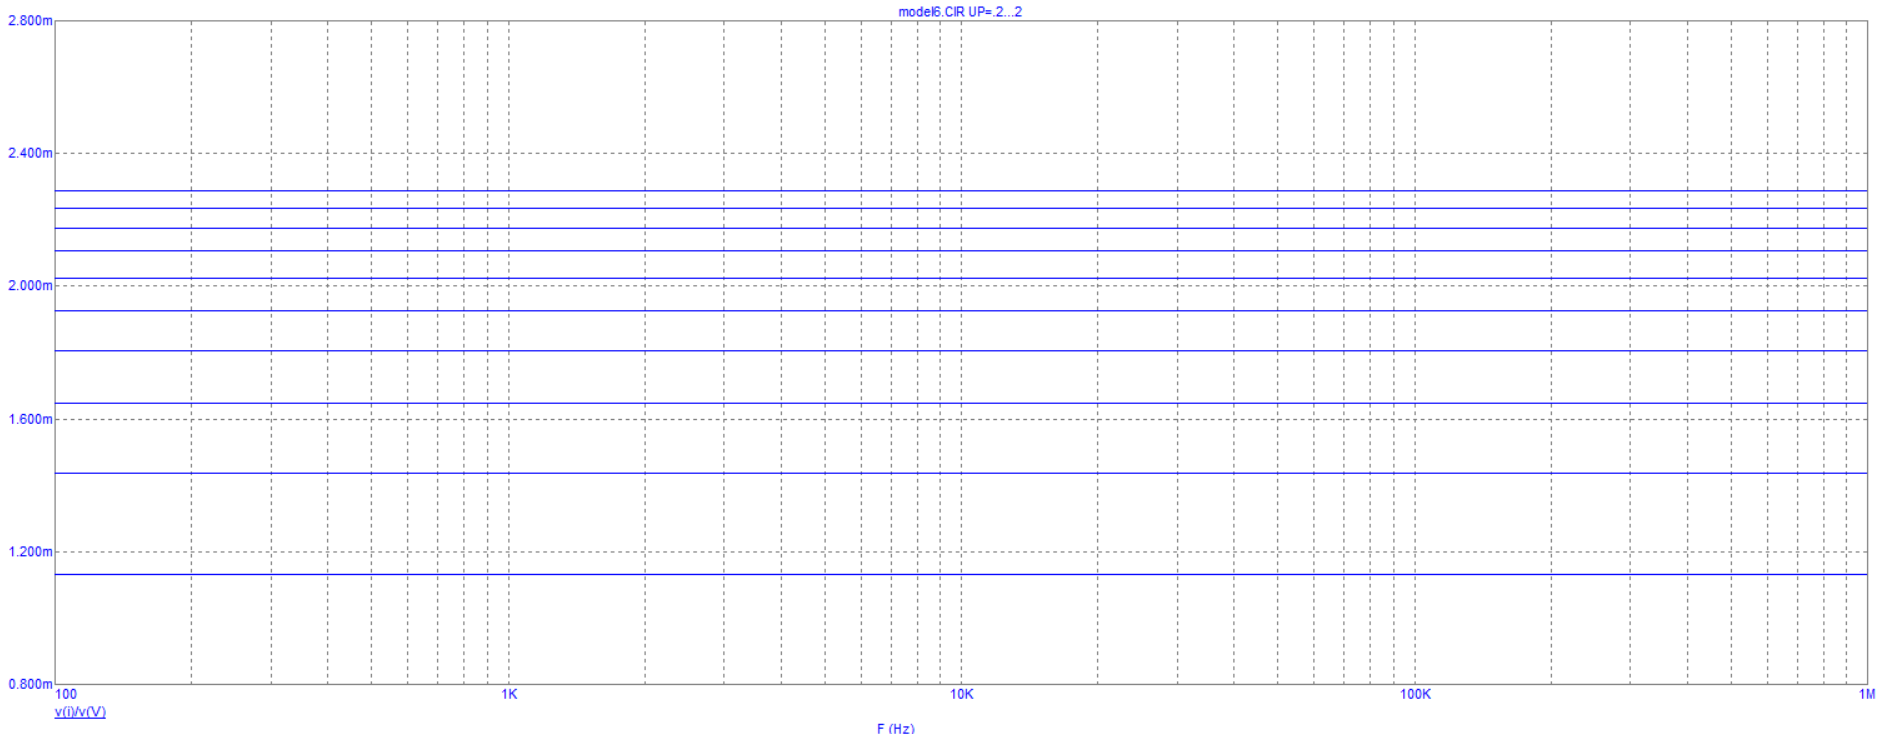
\includegraphics[scale = 0.4 \textwidth]{images/mod6_1_1.png}
    \caption{Крутизна транзистора}
    \label{fig:m611}
\end{figure}

\begin{table}[h!]
    \centering
    \begin{tabular}{|c|c|c|c|c|c|c|c|c|c|c|}
        $U_p$ & 2 & 1.8 & 1.6 & 1.4 & 1.2 & 1.0 & 0.8 & 0.6 & 0.4 & 0.2\\ \hline
        $S$ & 1.13 & 1.44 & 1.65 & 1.80 & 1.92 & 2.02 & 2.11 & 2.18 & 2.24 & 2.29 \\ \hline
    \end{tabular}
    \caption{Для $U_p = 1.1 V \, \frac{1}{S} \approx 0.5$}
    \label{tab:my_label}
\end{table}

\begin{figure}[h!]
    \centering
    \includegraphics[scale = 0.4 \textwidth]{images/mod6_1_2.png}
    \caption{Шумовой ток, варьирование $U_p$}
    \label{fig:m612}
\end{figure}

\begin{table}[h!]
    \centering
    \begin{tabular}{|c|c|c|c|c|c|c|c|c|c|c|}
        $U_p$ & 2.0 & 1.8 & 1.6 & 1.4 & 1.2 & 1.0 & 0.8 & 0.6 & 0.4 & 0.2\\ \hline
        $i_d$, p & 3.37 & 3.05 & 2.88 & 2.78 & 2.71 & 2.66 & 2.62 & 2.59 & 2.56 & 2.54 \\ \hline
    \end{tabular}
    \caption{Для $U_p = 1.1 V\, \gamma = \frac{i_d^2}{4kTS} \approx 0.65$}
    \label{tab:mt612}
\end{table}

\begin{figure}[h!]
    \centering
    \includegraphics[scale = 0.4 \textwidth]{images/mod6_1_3.png}
    \caption{Шумовой ток, варьирование Н}
    \label{fig:m613}
\end{figure}

\begin{table}[h!]
    \centering
    \begin{tabular}{|c|c|c|c|c|c|}
        $H$, Meg & 0 & 0.5 & 1 & 1.5 & 2\\ \hline
        $i_d$, n & 2.83 & 64.26 & 129.34 & 192.09 & 257.77 \\ \hline
    \end{tabular}
    \label{tab:mt613}
\end{table}
\FloatBarrier
\subsection{Исследование коэффициента шума}
\FloatBarrier
\begin{figure}
    \centering
    \includegraphics[scale = 0.4 \textwidth]{images/mod6_2_1.png}
    \caption{Напряжение на выходе, варьирование R}
    \label{fig:m621}
\end{figure}

\begin{table}[h!]
    \centering
    \begin{tabular}{|c|c|c|c|c|c|c|}
        $R$, k & 50 & 80 & 110 & 140 & 170 & 200\\ \hline
        $K_n$ & \\ \\hline
        $T_n$
    \end{tabular}
    \caption{}
    \label{tab:my_label}
\end{table}


\end{document}
